\documentclass[11pt,twoside,openany]{book}
\usepackage[utf8]{inputenc}
\usepackage[LGR,T1]{fontenc}
\usepackage{textalpha}
\usepackage[latin,italian]{babel}
\usepackage{ebgaramond}
\usepackage{microtype}
\usepackage[
  paperwidth=17cm,
  paperheight=24cm,
  inner=2.4cm,
  outer=2.6cm,
  top=2.6cm,
  bottom=2.8cm,
  headheight=14pt
]{geometry}
\usepackage[export]{adjustbox}
\usepackage{graphicx}
\usepackage{xcolor}
\usepackage{booktabs}
\usepackage{titlesec}
\usepackage{fancyhdr}
\usepackage[hidelinks,hypertexnames=false]{hyperref}

\definecolor{rubric}{RGB}{135,25,25}

\setlength{\parindent}{1.3em}
\setlength{\parskip}{0pt}
\raggedbottom

\pagestyle{fancy}
\fancyhf{}
\fancyhead[LE]{\small\scshape Galileo Galilei}
\fancyhead[RO]{\small\itshape Sidereus Nuncius}
\fancyfoot[C]{\thepage}
\renewcommand{\headrulewidth}{0.4pt}

\titleformat{\chapter}[display]
  {\normalfont\centering}
  {\large\scshape\color{rubric}\chaptertitlename\ \thechapter}
  {8pt}
  {\LARGE\scshape\color{rubric}}
\titlespacing*{\chapter}{0pt}{20pt}{25pt}

\begin{document}
\frontmatter

% --- FRONTESPIZIO ---
\begin{titlepage}
\centering
\vspace*{1cm}
{\Large\scshape Galileo Galilei\par}
\vspace{1.0cm}
{\Huge\scshape\color{rubric} Sidereus Nuncius\par}
\vspace{0.4cm}
{\Large\scshape Avviso Astronomico\par}
\vspace{0.8cm}
{\normalsize che contiene e spiega le grandi e oltremodo mirabili osservazioni\\
fatte da\par}
\vspace{0.3cm}
{\large\scshape Galileo Galilei\par}
{\small Patrizio Fiorentino e Pubblico Matematico dello Studio di Padova\par}
\vspace{0.4cm}
{\normalsize con l'aiuto del cannocchiale da lui recentemente inventato,\\
nella faccia della Luna, in innumerevoli Stelle fisse, nella Via Lattea, nelle Stelle nebulose,\\
ma soprattutto in\par}
\vspace{0.3cm}
{\large\scshape\color{rubric} Quattro Pianeti\par}
{\normalsize che ruotano intorno alla stella di Giove ad intervalli e periodi disuguali\\
con meravigliosa celerità; i quali, da nessuno conosciuti fino a questo giorno,\\
l'Autore per primo scoprì recentemente e stabilì di nominare\par}
\vspace{0.3cm}
{\large\scshape Astri Medicei\par}
\vfill
\rule{0.45\textwidth}{0.4pt}\\[0.5cm]
{\scshape In Venezia $\cdot$ MDCX\par}
{\small\itshape Presso Tommaso Baglioni\par}
\vspace{0.6cm}
{\footnotesize Edizione bilingue (Traduzione italiana e Testo originale latino) in \LaTeX\par}
\end{titlepage}

% --- NOTA FILOLOGICA ---
\chapter*{Nota Filologica ed Editoriale}
\addcontentsline{toc}{chapter}{Nota Filologica ed Editoriale}
{\small
La presente edizione bilingue del \textit{Sidereus Nuncius} di Galileo Galilei (Venezia, Tommaso Baglioni, 1610) comprende sia la traduzione italiana (\textit{Avviso Astronomico}) di Luisa Lanzillotta sia il testo originale latino (\textit{Sidereus Nuncius / Astronomicus Nuncius}), condotti sull'Edizione Nazionale delle Opere di Galileo Galilei (vol.~III, parte~I, a cura di Antonio Favaro, Firenze, Barbèra, 1892) e sull'edizione critica a cura di Ferdinando Flora (\textit{Opere}, Milano-Napoli, Riccardo Ricciardi Editore, 1953).

L'apparato iconografico riproduce integralmente tutte le 71 tavole e figure astronomiche originali:
\begin{itemize}
\item le cinque incisioni selenografiche delle fasi lunari e del rilievo anulare centrale;
\item il diagramma geometrico per la determinazione trigonometrica dell'altezza delle montagne lunari (oltre quattro miglia italiane);
\item le mappe celesti della Cintura e della Spada d'Orione, delle Pleiadi, della Nebulosa del Capo d'Orione e della Nebulosa del Presepe;
\item la serie completa delle 65 configurazioni osservative dei quattro satelliti galileiani di Giove (\textit{Medicea Sidera}), registrate dal 7~gennaio al 2~marzo 1610.
\end{itemize}
}

\tableofcontents

\mainmatter

% =========================================================================
% PARTE I: TRADUZIONE ITALIANA (AVVISO ASTRONOMICO)
% =========================================================================
\part*{Parte Prima\\{\Large\scshape\color{rubric} Avviso Astronomico}\\{\normalsize\itshape Traduzione italiana di Luisa Lanzillotta}}
\addcontentsline{toc}{part}{Parte Prima: Avviso Astronomico (Traduzione italiana)}

\chapter*{Al Serenissimo Cosimo II de' Medici IV Granduca di Toscana}
\addcontentsline{toc}{chapter}{Al Serenissimo Cosimo II de' Medici IV Granduca di Toscana}

Insigne istituzione certo e assai civile fu quella di coloro che tentarono di proteggere dall'invidia le opere famose di uomini eccellenti per virtù e salvare dall'oblio e dalla morte i nomi loro degni d'immortalità. Perciò si tramandarono alla memoria dei posteri immagini scolpite nel marmo o fuse in bronzo, perciò si posero statue pedestri ed equestri, perciò le spese per colonne e piramidi giunsero, come disse il poeta, alle stelle, per questo infine si costruirono le città e fu loro imposto il nome di quelli che i grati posteri vollero imperituri. Tale è infatti la condizione dell'umana mente che, se non è stimolata da immagini che di continuo le si presentino dall'esterno, ogni ricordo facilmente svanisce.

Alcuni però che guardano a cose più salde e durature consacrarono la fama eterna di uomini sommi non a marmi o metalli, ma alla custodia delle Muse e agli incorrotti monumenti delle lettere. Ma perché ricordo queste cose? quasi che l'ingegno umano, contento di queste regioni, non abbia osato andar oltre: invece, guardando più lontano, avendo ben compreso che tutti i monumenti umani per violenza di tempeste o per vecchiezza alfine muoiono, pensò più incorruttibili monumenti, sui quali il tempo vorace e l'invidiosa vecchiezza non potessero reclamare diritti. E scrutando il cielo affidò a quei noti eterni Globi di chiarissime Stelle i nomi di coloro che per opere egrege e quasi divine furono stimati degni di godere insieme agli Astri l'eternità. Per questo non si oscurerà la fama di Giove, Marte, Mercurio, Ercole e degli altri eroi con i cui nomi si chiamano le Stelle, prima che lo splendore delle stesse Stelle. Tuttavia questa invenzione dell'umano ingegno, tra le prime mirabile e nobile, già da molti secoli è spenta, occupando i primi eroi quelle lucenti sedi e come per proprio diritto tenendole: nel loro numero invano la pietà di Augusto tentò di eleggere Cesare: infatti, volendo egli chiamare Astro Giulio la stella apparsa al tempo suo, di quelle che i Greci chiamano Comete, i Latini Crinite, quella scomparendo in breve tempo deluse la speranza. Ma cose di gran lunga più felici e vere, Serenissimo Principe, possiamo predire alla vostra Altezza: infatti appena han cominciato a rifulgere in terra le bellezze immortali del vostro animo, e si mostrano in cielo lucenti Stelle che come lingue celebrino e dicano in ogni tempo le mirabili vostre virtù. Ecco dunque quattro Stelle riservate al vostro inclito nome e non del numero gregario e meno insigne delle fisse, ma dell'ordine illustre dei Pianeti che con moto diverso, attorno a Giove nobilissima Stella, come progenie sua schietta, compiono l'orbita loro con celerità mirabile, e nello stesso tempo con unanime concordia compiono tutte insieme ogni dodici anni grandi rivoluzioni attorno al centro del mondo, cioè al Sole. E lo stesso Artefice delle Stelle parve con segni manifesti invitarmi a dedicare al nome eccelso della vostra Altezza piuttosto che ad altri questi nuovi Pianeti. Infatti, come queste Stelle, quasi prole degna di Giove, non si staccano mai dal suo fianco se non di poco, così chi ignora che la clemenza, la mitezza d'animo, la soavità dei modi, lo splendore del regio sangue, la maestà delle azioni, l'eccellenza dell'autorità e dell'imperio, che tutte collocaron domicilio e sede nella vostra Altezza, chi, dico, ignora che tutte queste virtù emanano dal benignissimo Astro di Giove, dopo Dio fonte suprema d'ogni bene? Giove, Giove, dico, al primo sorgere della vostra Altezza, già passato oltre i torbidi vapori dell'orizzonte, occupando il mezzo del cielo e illuminando con la sua reggia l'angolo orientale, mirò da quel sublime trono il felicissimo parto, e tutto il suo splendore e la grandezza sua profuse nell'aere purissimo, perché il tenero corpo insieme con l'anima ornata da Dio dei più nobili ornamenti bevesse col primo respiro quell'universale forza e potere. Invero perché mi valgo di argomenti probabili quando potrei concludere e dimostrare con un argomento quasi inoppugnabile? Piacque a Dio Ottimo Massimo che dai Serenissimi vostri genitori non fossi stimato indegno di istruire nelle Matematiche la vostra Altezza, il che adempii nei quattro anni passati, nel tempo dell'anno in cui si è soliti riposarsi dagli studi più severi. E poiché, certo per divino consiglio, mi fu dato in sorte di servire la vostra Altezza e ricevere tanto da vicino i raggi dell'incredibile vostra clemenza e benignità, che meraviglia se l'animo mio si scaldò tanto che nulla il giorno o la notte pensava se non il modo con cui io, che non solo per l'animo, ma anche per nascita e natura vi sono soggetto, mi mostrassi cupidissimo della vostra gloria ed a voi gratissimo? E quando accadde che, sotto i vostri auspicii, Serenissimo Cosimo, scoprii queste Stelle ignote a tutti i precedenti Astronomi, ben a ragione decisi di insignirle dell'Augustissimo nome della vostra Casa. Che se io per primo le studiai, chi ragionevolmente mi riprenderà se imporrò loro anche un nome e le chiamerò ASTRI MEDICEI? nella speranza che da questo nome verrà a questi Astri tanto onore quanto gli altri ne recarono agli altri Eroi. Infatti, per tacere dei Serenissimi vostri Antenati, la cui sempiterna gloria testimoniano i monumenti di tutte le storie, la sola vostra virtù, Massimo Eroe, può dare a quegli Astri l'immortalità del nome. Chi infatti può aver dubbio che l'aspettazione che del vostro impero suscitaste con felicissimi auspicii, quantunque somma, non solo manteniate alta e custodiate, ma siate per superare in lungo intervallo di tempo? sì che quando avrete superato tutti i vostri simili, gareggerete con voi stesso, e di voi e della grandezza vostra sarete di giorno in giorno maggiore.

Accogliete dunque, Clementissimo Principe, questa gloria gentilizia a voi riservata dagli Astri, e di quei beni divini che non tanto dalle Stelle quanto dal loro Fattore e Moderatore Dio vi son largiti godete quanto più a lungo possibile.

Padova, 12 Marzo 1610.

Dell'Altezza Vostra

Devotissimo servo

Galileo Galilei.

\chapter*{Licenza dei Capi del Consiglio dei Dieci}
\addcontentsline{toc}{chapter}{Licenza dei Capi del Consiglio dei Dieci}

Gli Eccellentissimi Signori Capi dell'Ecc. Cons. de' X infrascritti, avuta fede dalli Signori Reformatori del Studio di Padova per relazione delli due a questo deputati, cioè dal Rever. P. Inquisitor, e dal circospetto Secretario del Senato, Gio. Maraviglia, con giuramento, come nel libro intitolato: SIDEREUS NUNCIUS etc. di D. Galileo Galilei non si trova alcuna cosa contraria alla Santa Fede Cattolica, Prencipi e buoni costumi, e che è degno di stampa, concedono licenza che possi esser stampato in questa Città.

Datum die primo Martii 1610.

\begin{center}
$\left.\begin{tabular}{@{}l@{}}
D. M. Ant. Valaresso \\
D. Nicolò Bon \\
D. Lunardo Marcello
\end{tabular}\right\}$ \textit{Capi dell'Ecc. Cons. de' X}
\end{center}

Illustrissimi Consilii X Secretarius

Bartholomæs Cominus.

1610, a dì 8 Marzo. Regist. in libro a car. 39.

Ioan. Baptista Breatto off.

Con. Blasph. Coad.

\chapter{Avviso Astronomico}
\begin{center}
{\itshape Osservazioni recentemente fatte con l'aiuto di un nuovo occhiale nella faccia della Luna, nella Via Lattea e nelle Nebulose, nelle innumerevoli Stelle fisse, ed anche nei quattro Pianeti chiamati Astri Medicei, mai fino ad ora visti\par}
\end{center}
\bigskip

Grandi cose per verità in questo breve trattato propongo all'osservazione e alla contemplazione di quanti studiano la natura. Grandi, dico, e per l'eccellenza della materia stessa, e per la novità non mai udita nei secoli, e infine per lo strumento mediante il quale queste cose stesse si sono palesate al nostro senso.

Grande cosa è certamente alla immensa moltitudine delle stelle fisse che fino a oggi si potevano scorgere con la facoltà naturale, aggiungerne e far manifeste all'occhio umano altre innumeri, prima non mai vedute e che il numero delle antiche e note superano più di dieci volte.

Bellissima cosa e mirabilmente piacevole, vedere il corpo della Luna, lontano da noi quasi sessanta raggi terrestri, così da vicino come distasse solo due di queste dimensioni; così che si mostrano il diametro stesso della Luna quasi trenta volte, la sua superficie quasi novecento, il volume quasi ventisettemila volte maggiori che quando si guardano a occhio nudo: e quindi con la certezza della sensata esperienza chiunque può comprendere che la Luna non è ricoperta da una superficie liscia e levigata, ma scabra e ineguale, e, proprio come la faccia della Terra, piena di grandi sporgenze, profonde cavità e anfratti.

Inoltre non mi pare si debba stimar cosa da poco l'aver rimosso le controversie intorno alla Galassia, o Via Lattea, e aver manifestato al senso oltre che all'intelletto l'essenza sua; e inoltre il mostrare a dito che la sostanza degli astri fino a oggi chiamati dagli astronomi nebulose è di gran lunga diversa da quel che si è fin qui creduto, sarà cosa grata e assai bella.

Ma quel che di gran lunga supera ogni meraviglia, e principalmente ci spinse a renderne avvertiti tutti gli astronomi e filosofi, è l'aver scoperto quattro astri erranti, da nessuno, prima di noi, conosciuti né osservati, che, a somiglianza di Venere e Mercurio intorno al Sole, hanno le loro rivoluzioni attorno a un certo astro cospicuo tra i conosciuti, ed ora lo precedono ora lo seguono, non mai allontanandosene oltre determinati limiti. E tutte queste cose furono scoperte e osservate pochi giorni or sono con l'aiuto d'un occhiale che io inventai dopo aver ricevuto l'illuminazione della grazia divina.

Altre cose più mirabili forse da me e da altri si scopriranno in futuro con l'aiuto di questo strumento, della cui forma e struttura e dell'occasione d'inventarlo dirò prima brevemente, poi narrerò la storia delle osservazioni da me fatte.

Circa dieci mesi fa ci giunse notizia che era stato costruito da un certo Fiammingo un occhiale, per mezzo del quale gli oggetti visibili, pur distanti assai dall'occhio di chi guarda, si vedevan distintamente come fossero vicini; e correvan voci su alcune esperienze di questo mirabile effetto, alle quali chi prestava fede, chi no. Questa stessa cosa mi venne confermata pochi giorni dopo per lettera dal nobile francese Iacopo Badovere, da Parigi; e questo fu causa che io mi volgessi tutto a cercar le ragioni e ad escogitare i mezzi per giungere all'invenzione di un simile strumento, che poco dopo conseguii, basandomi sulla dottrina delle rifrazioni. Preparai dapprima un tubo di piombo alle cui estremità applicai due lenti, entrambe piane da una parte, e dall'altra una convessa e una concava; posto l'occhio alla parte concava vidi gli oggetti abbastanza grandi e vicini, tre volte più vicini e nove volte più grandi di quanto non si vedano a occhio nudo. In seguito preparai uno strumento più esatto, che mostrava gli oggetti più di sessanta volte maggiori. E finalmente, non risparmiando fatiche e spese, venni a tanto da costruirmi uno strumento così eccellente, che gli oggetti visti per il suo mezzo appaiono ingranditi quasi mille volte e trenta volte più vicini che visti a occhio nudo. Quanti e quali siano i vantaggi di un simile strumento, tanto per le osservazioni di terra che di mare, sarebbe del tutto superfluo dire. Ma lasciate le terrestri, mi volsi alle speculazioni del cielo; e primamente vidi la Luna così vicina come distasse appena due raggi terrestri. Dopo questa, con incredibile godimento dell'animo, osservai più volte le stelle sia fisse che erranti; e poiché le vidi assai fitte, cominciai a studiare il modo con cui potessi misurare le loro distanze, e finalmente lo trovai. Su questo è bene siano avvertiti tutti coloro che vogliono darsi a simili osservazioni. In primo luogo è necessario infatti che si preparino un cannocchiale esattissimo, il quale rappresenti gli oggetti chiari, distinti e non coperti d'alcuna caligine, e li ingrandisca almeno quattrocento volte, poiché allora li mostrerà venti volte più vicini: infatti, se lo strumento non sarà tale, invano si tenterà di vedere tutte le cose che da me furon viste in cielo, e che più avanti saranno enumerate. Affinché chiunque con poca fatica possa farsi certo dell'ingrandimento dello strumento, tracci il contorno di due circoli o due quadrati di carta, di cui l'uno sia quattrocento volte maggiore dell'altro; il che sarà quando il diametro del maggiore avrà lunghezza venti volte più grande del diametro dell'altro: poi guardi insieme da lontano le due superfici infisse alla stessa parete, la minore con un occhio posto al cannocchiale, la maggiore con l'altro occhio, libero. Senza fatica infatti questo si può fare nel medesimo tempo, tenendo aperti tutti e due gli occhi: entrambe le figure appariranno allora della stessa grandezza, se il cannocchiale moltiplicherà gli oggetti secondo la proporzione voluta. Preparato simile strumento, bisognerà studiare il modo di misurare le distanze: cosa che otterremo col seguente artificio. Sia, per maggior semplicità, il tubo ABCD.

\begin{center}\vspace{0.35em}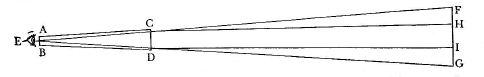
\includegraphics[max width=0.82\textwidth,max height=0.45\textheight,keepaspectratio]{images/figura05.png}\vspace{0.35em}\end{center}
L'occhio di colui che guarda sia E. I raggi, finché non ci sono nel cannocchiale le lenti, giungono all'oggetto FG secondo le linee rette ECF, EDG; ma, poste le lenti, giungeranno secondo le linee rifratte ECH, EDI: infatti sono raccostati, e quelli che prima, liberi, si dirigevano all'oggetto FG, ne comprenderanno solo la parte HI. Trovato poi il rapporto della distanza EH alla linea HI, con la tavola dei seni si troverà l'ampiezza dell'angolo formato nell'occhio dall'oggetto HI, che vedremo contenere soltanto qualche minuto. Se poi adatteremo alla lente CD sottili lamine, perforate alcune con fori maggiori altre con fori minori, sovrapponendo or questa or quella secondo sarà necessario, formeremo a piacere angoli diversi, sottendenti più o meno minuti, con l'aiuto dei quali potremo facilmente misurare gli intervalli fra le Stelle, distanti l'una dall'altra di qualche minuto, senza errore nemmeno di uno o due minuti. Ma per il momento basti aver toccato di questi argomenti così lievemente, e quasi averne gustato a fior di labbra, poiché in altra occasione esporremo intera la teoria di questo strumento.

Ora verremo esponendo le osservazioni da noi fatte nei due mesi trascorsi, richiamando, agli esordi di così grandi contemplazioni, l'attenzione di tutti quanti amano la vera filosofia.

In primo luogo diremo dell'emisfero della Luna che è volto verso di noi. Per maggior chiarezza divido l'emisfero in due parti, più chiara l'una, più scura l'altra: la più chiara sembra circondare e riempire tutto l'emisfero, la più scura invece offusca come nube la faccia stessa e la fa apparire cosparsa di macchie. Queste macchie alquanto scure e abbastanza ampie, ad ognuno visibili, furono scorte in ogni tempo; e perciò le chiameremo grandi o antiche, a differenza di altre macchie minori per ampiezza ma pure così frequenti da coprire l'intera superficie lunare, soprattutto la parte più luminosa: e queste non furono viste da altri prima di noi. Da osservazioni più volte ripetute di tali macchie fummo tratti alla convinzione che la superficie della Luna non è levigata, uniforme ed esattamente sferica, come gran numero di filosofi credette di essa e degli altri corpi celesti, ma ineguale, scabra e con molte cavità e sporgenze, non diversamente dalla faccia della Terra, variata da catene di monti e profonde valli. Le cose che vidi e da cui potei trarre queste conclusioni, sono le seguenti:

Nel quarto o quinto giorno dopo la congiunzione, quando la Luna ci mostra i corni splendenti, il termine di divisione tra la parte scura e la chiara non si stende uniformemente secondo una linea ovale, come accadrebbe in un solido perfettamente sferico, ma è tracciato da una linea ineguale, aspra e assai sinuosa. Infatti molte luminosità come escrescenze si estendono oltre i confini della luce e delle tenebre, e per contro alcune particelle oscure si introducono nella parte illuminata. Di più: anche gran copia di piccole macchie nerastre, del tutto separate dalla parte oscura, cospargono quasi tutta la plaga già illuminata dal Sole, eccettuata soltanto quella parte che è cosparsa di macchie grandi e antiche. Notammo pure che le suddette piccole macchie concordano, tutte e sempre, in questo: nell'avere la parte nerastra volta al luogo del Sole; nella parte opposta al Sole invece sono coronate da contorni lucentissimi, quasi montagne accese. Uno spettacolo simile abbiamo sulla Terra verso il sorgere del Sole quando vediamo le valli non ancora illuminate e splendenti i monti che le circondano dalla parte opposta al Sole: e come le ombre delle cavità terrestri di mano in mano che il Sole si innalza si fanno più piccole, così anche queste macchie lunari, al crescere della parte luminosa, perdono le tenebre.\footnote{\textsuperscript{Vedi figura 1.}}


\begin{center}\vspace{0.6em}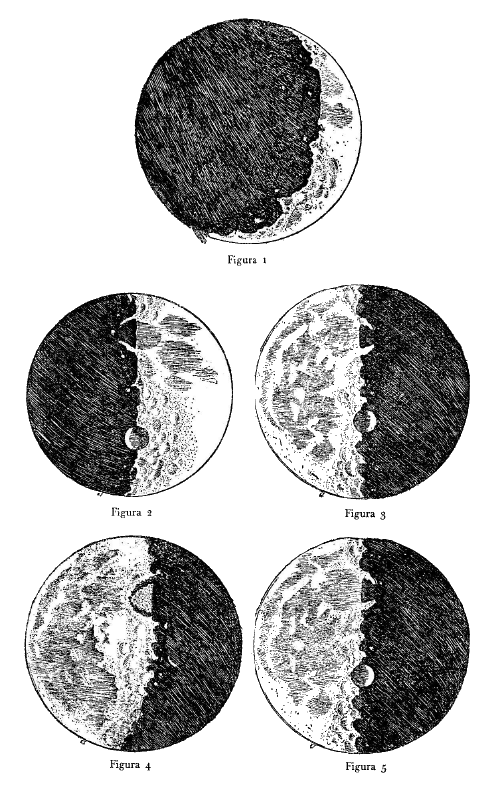
\includegraphics[max width=0.88\textwidth,max height=0.72\textheight,keepaspectratio]{images/figura01.png}\vspace{0.6em}\end{center}


Veramente non solo i confini tra luce e tenebre si scorgono nella Luna ineguali e sinuosi, ma – ciò che desta maggior meraviglia – nella parte tenebrosa della Luna si mostrano moltissime cuspidi lucenti, completamente divise e avulse dalla parte illuminata e lontane da questa non piccolo tratto: che a poco a poco, dopo un certo tempo, aumentano di grandezza e luminosità: dopo due o tre ore si congiungono alla restante parte luminosa già divenuta più grande; frattanto altre e altre punte come pullulanti qua e là si accendono nella parte tenebrosa, ingrandiscono e infine si congiungono anch'esse alla parte luminosa che si è venuta sempre più ampliando. La figura precedente ci offre un esempio anche di questo fenomeno. E sulla Terra, prima che si levi il Sole, mentre ancora l'ombra occupa le pianure, le cime dei monti più alti non sono forse illuminate dai raggi solari? non s'accresce in breve tempo la luce, quando le parti medie e le più larghe dei monti si illuminano: e finalmente, sorto già il Sole, non si congiungono le illuminazioni delle pianure e dei colli? Le varietà di tali protuberanze e cavità della Luna, sembrano poi superare d'assai l'asperità della superficie terrestre, come dimostreremo più innanzi. Frattanto non passerò sotto silenzio un fatto degno di attenzione che osservai mentre la Luna si avviava al primo quarto, come la mostra il disegno che sopra abbiamo riprodotto: nella parte luminosa penetra un grande seno oscuro, collocato verso il corno inferiore, il qual seno avendo io a lungo osservato e scorto del tutto oscuro, finalmente dopo circa due ore cominciò a spuntare, poco sotto il mezzo della sinuosità, una sorta di vertice luminoso; questo a poco a poco crescendo prendeva figura triangolare e rimaneva del tutto staccato e separato dalla faccia luminosa; poco dopo attorno a quello cominciarono a luccicare tre piccole punte, fino a che, volgendo già la Luna al tramonto, la figura triangolare, estesa e fatta più ampia, si univa alla rimanente parte luminosa e grande come un grande promontorio, ancora circondata dai tre punti ricordati, si diffondeva nel seno tenebroso. Inoltre, all'estremità dei corni, sia superiore che inferiore, emergevano alcuni punti luminosi e completamente disgiunti dall'altra parte luminosa, come si vede rappresentato nella figura precedente. Nell'uno e nell'altro corno era gran quantità di macchie scure, sopra tutto nell'inferiore; ed appaiono più grandi e oscure le più vicine al limite tra luce e tenebre, le più lontane meno oscure e più sbiadite. Sempre però, come anche sopra ricordammo, la parte nericcia della macchia è rivolta verso l'irradiazione solare, mentre un contorno luminoso circonda la macchia nericcia dalla parte opposta al Sole e rivolta alla parte oscura della Luna. Questa superficie lunare, là dove è variata da macchie, come occhi cerulei d'una coda di pavone, appare simile a quei vasetti di vetro che, posti ancora incandescenti in acqua fredda, acquistan superficie screpolata e ineguale, onde son detti dal volgo bicchieri di ghiaccio. Invero le grandi macchie della Luna non si vedono così rotte e ricche di avvallamenti e sporgenze, ma più uguali e uniformi; infatti spuntano solo qua e là piccole zone più luminose, cosicché se qualcuno volesse riesumare l'antica opinione dei pitagorici, cioè che la Luna sia quasi una seconda Terra, la parte di essa più luminosa rappresenterebbe meglio la superficie solida, la più scura quella acquea; e non mai ebbi dubbio che, guardato da lontano, il globo terrestre illuminato dal Sole, la superficie terrea si presenterebbe più chiara, più scura la parte acquea. Inoltre nella Luna le grandi macchie si scorgono maggiormente depresse delle parti più luminose; infatti, sia la Luna crescente o calante, sempre al limite fra luce e tenebre sporgono attorno alle grandi macchie i contorni della parte più luminosa, come osservammo nell'illustrare le figure; e i confini di quelle macchie non sono soltanto più depressi, ma anche più eguali e non interrotti da pieghe o asperità. La parte più luminosa invero sporge sopra tutto in vicinanza delle macchie, così che avanti la prima quadratura, e assai probabilmente anche nella seconda, attorno a una certa macchia posta nella parte superiore o boreale della Luna, si ergono notevolmente sopra e sotto di quella grandi sporgenze, come mostrano le figure.\footnote{\textsuperscript{Vedi figure 2 e 3.}}

Questa macchia medesima si vede, avanti la seconda quadratura, circondata da contorni più oscuri che, come catene altissime di monti, si mostran più scuri dalla parte opposta al Sole, più luminosi in quella rivolta al Sole: accade l'opposto invece nelle cavità, delle quali appare splendente la parte opposta al Sole, oscura ed ombrosa quella situata dalla parte del Sole. Fatta più piccola la superficie luminosa, quantunque dapprima quasi tutta la detta macchia sia coperta d'ombra, emergon più chiari oltre le tenebre i dorsi dei monti. Questo duplice aspetto mostrano le figure.\footnote{\textsuperscript{Vedi figure 4 e 5.}}

E voglio anche ricordare un'altra cosa che notai non senza una certa meraviglia: quasi nel mezzo della Luna vi è una cavità maggiore di tutte le altre e perfettamente rotonda di figura: questa scorsi in vicinanza di entrambe le quadrature, e per quanto mi fu possibile riprodussi nelle due figure poste qui sopra: per quel che riguarda l'adombramento e l'illuminazione offre lo stesso aspetto che sulla Terra offrirebbe la regione consimile della Boemia, se fosse da ogni parte circondata da monti altissimi, e disposti a circolo perfetto; nella Luna infatti è circondata da monti così alti che la regione estrema confinante con la parte tenebrosa di essa si vede illuminata dal raggio solare prima che il limite tra la luce e l'ombra raggiunga il diametro della figura stessa. Come nelle altre macchie, la parte ombrosa di quella guarda il Sole, la parte luminosa è volta verso la parte oscura della Luna; per la terza volta richiamo l'attenzione su questo, come su una inoppugnabile testimonianza delle asperità e ineguaglianze che sono su tutta la parte più chiara della Luna: tra queste macchie, sempre le più scure sono quelle vicine al confine tra luce e tenebre; le più lontane invece appaiono ora più piccole, ora meno oscure; così che, quando la Luna, all'opposizione, è piena, assai poca differenza corre tra l'oscurità degli avvallamenti e il fulgore delle cime.

Le cose che abbiamo riferito si osservano nella parte più luminosa della Luna; nelle grandi macchie non si vede tanta differenza di cavità e sporgenze, quale arguimmo necessario porre nella parte più luminosa per il mutare delle configurazioni col variare dall'una all'altra delle illuminazioni del Sole, secondo le molteplici posizioni dalle quali esso guarda la Luna: nelle grandi macchie invece esistono brevi aree leggermente più scure, come notammo nelle figure; tuttavia esse si mostran sempre uguali, né aumenta o diminuisce la loro opacità, ma con differenze minime appaiono ora più scure, ora più chiare, a seconda che i raggi del Sole incidono in esse più o meno obliqui: le congiunge inoltre con le parti vicine delle macchie una specie di lieve legame, e mescolano e confondono i confini. Diversamente invece accade nelle macchie occupanti la superficie più chiara della Luna: infatti come rupi erte e con aspri ed angolosi scogli, si staccano l'una dall'altra con netti contrasti di luci ed ombre. Tra queste grandi macchie si vedono piccole aree, alcune chiare e alcune perfino lucentissime: invero queste e quelle più scure hanno sempre uguale aspetto e nessuna mutazione di figura, luce, opacità: così da non esser più dubbio che quelle appaiono per una reale disuguaglianza delle parti e non soltanto per ineguaglianze nei loro aspetti in conseguenza delle diverse illuminazioni del Sole, moventi le ombre in modi diversi, come accade invece nelle altre macchie minori che occupano la parte più chiara della Luna. Quelle di giorno in giorno cambiano aspetto, aumentano, diminuiscono, scompaiono, poiché traggono origine soltanto dalle ombre delle parti elevate.

Ma a questo proposito so che molti sono grandemente perplessi, e colpiti da una difficoltà tanto grave da costringerli a revocare in dubbio una conclusione spiegata e confermata da tante apparenze. Se infatti quella parte della superficie lunare che più luminosamente rimanda i raggi ha tanti anfratti, protuberanze e avvallamenti, perché, quando la Luna cresce, le parti estreme che guardano a occidente, e, quando decresce, quelle rivolte a oriente, e, nel plenilunio, tutta la circonferenza, non si vede ineguale, scabra e sinuosa, ma esattamente circolare, e senza protuberanza alcuna né cavità? Tanto più che l'orlo intero si compone della sostanza più chiara della Luna, che dicemmo tutta prominenze e cavità; infatti nessuna delle grandi macchie si spinge fino al limite estremo della circonferenza, ma tutte si vedono radunate lontane dall'orlo.

Espongo la duplice causa di questo fenomeno, che offre appiglio a dubbi tanto gravi, dando perciò duplice spiegazione al dubbio. In primo luogo se le protuberanze e le cavità del corpo lunare si estendessero solo secondo la circonferenza terminale dell'emisfero a noi visibile, allora la Luna potrebbe, anzi dovrebbe mostrarsi a noi quasi simile a ruota dentata, col contorno ricco di bozze e sinuoso: però se non una sola catena di monti disposta unicamente intorno alla circonferenza, ma molte file di monti con loro valli e anfratti si trovano disposti parallelamente attorno alla periferia della Luna, e non solo nell'emisfero visibile, ma anche in quello invisibile (sempre presso il confine tra l'uno e l'altro), allora un occhio che guardi da lontano non potrà assolutamente vedere il distacco tra le parti elevate e le cavità, perché gli intervalli tra i monti disposti nello stesso cerchio, cioè nella medesima serie, sono nascosti da altri monti disposti in altre e altre file, soprattutto se l'occhio di chi guarda sarà posto sulla stessa retta con le cime delle dette elevazioni. Così sulla Terra i gioghi di molti e fitti monti appaiono disposti su una stessa superficie piana se colui che guarda sta lontano e ad eguale altezza. Allo stesso modo i vertici delle onde di un mare tempestoso sembran distesi secondo uno stesso piano, quantunque tra i flutti sia assai grande frequenza di voragini e lacune, tanto profonde che tra esse si nascondono non solo le carene, ma le poppe, gli alberi e le vele di grandi navi. Poiché infatti nella Luna e intorno al suo perimetro sono molti ordini di prominenze e avvallamenti, e l'occhio che guarda da lontano è posto quasi sullo stesso piano dei vertici di quelle prominenze: nessuno deve meravigliarsi che allo sguardo che li sfiora si presentino secondo una linea uniforme e per nulla anfrattuosa. A questa spiegazione se ne può aggiungere un'altra: attorno al corpo lunare come attorno alla Terra c'è una specie d'involucro di sostanza più densa dell'altra aria, che ha potere di accogliere e riflettere le irradiazioni solari, quantunque non sia tanto opaco da impedire alla vista (soprattutto fin quando non è illuminato) di passare. Questo involucro, illuminato dai raggi solari, rende e mostra la Luna come una sfera più grande, e potrebbe impedirci di penetrare con lo sguardo sino alla parte solida della Luna se fosse di maggior spessore: e di maggior spessore è intorno all'orlo della Luna; non in senso assoluto, ma perché così giunge ai nostri sguardi che lo secano obliquamente: e per questo può impedire la nostra vista e, soprattutto se luminoso, celare l'orlo della Luna esposto al Sole. Cosa che s'intende più chiaramente nella figura apposta, nella quale il corpo lunare ABC è circondato dal globo vaporoso DEG; l'occhio arriva da F alle parti intermedie della Luna, come ad A, attraverso i vapori DA meno profondi: ma verso la periferia estrema una quantità di più densi vapori EB impedisce col suo confine il nostro sguardo. Di questo è indice il fatto che la parte della Luna pervasa di luce appare di più grande circonferenza che il resto del globo oscuro: e taluno stimerà questa stessa la causa razionale per cui le più grandi macchie della Luna non sembrano protendersi da nessuna parte fino all'estremo orlo, quantunque si possa pensare che se ne trovino anche attorno a quello; sembra però credibile che siano di poca entità dato che si nascondono sotto una più densa e luminosa massa di vapori.

\begin{center}\vspace{0.35em}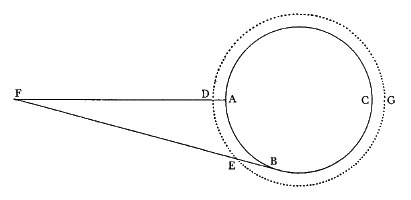
\includegraphics[max width=0.82\textwidth,max height=0.45\textheight,keepaspectratio]{images/figura06.png}\vspace{0.35em}\end{center}
Che dunque la superficie più chiara della Luna sia cosparsa ovunque di rigonfiamenti e avvallamenti, credo sia manifestato a sufficienza dai fenomeni già spiegati. Rimane da dire delle loro grandezze, che dimostrano come le asperità terrestri siano assai minori di quelle lunari; minori, dico, anche parlando in senso assoluto, non in rapporto soltanto alle dimensioni dei globi terrestre e lunare: e questo si dimostra chiaramente così.

Avendo io più e più volte osservato, in diverse posizioni della Luna rispetto al Sole, che nella parte tenebrosa della Luna alcuni vertici, anche se abbastanza lontani dal confine della luce, ne apparivan pervasi, mettendo a raffronto la loro distanza con l'intero diametro della Luna, accertai che questa distanza supera talvolta la ventesima parte del diametro. Stabilito questo, si pensi il globo lunare, il cui circolo massimo sia CAF, il centro E, il diametro CF, che sta al diametro della terra come due a sette; poiché il diametro terrestre, secondo le più esatte osservazioni, misura 7000 miglia italiane, sarà CF 2000, CE 1000, la ventesima parte di tutto CF 100 miglia. Sia ora CF il diametro del circolo massimo, che divide la parte luminosa della Luna da quella oscura (infatti per la grandissima lontananza del Sole dalla Luna questo circolo non differisce sensibilmente dal circolo massimo) e A disti dal punto C la ventesima parte di quel diametro: si prolunghi il semidiametro EA, fino all'incontro nel punto D della tangente GCD (che rappresenta il raggio illuminante). Sarà dunque l'arco CA, o il segmento CD, 100 di tali parti delle quali CE è 1000, e la somma dei quadrati di DC e di CE 1.010.000, alla quale è uguale il quadrato di DE: dunque tutta ED sarà più di 1004, e AD più di 4 di tali parti, delle quali CE è 1000. Nella Luna dunque l'altezza AD, che designa un qualsiasi vertice elevato fino al raggio solare GCD e lontano dal confine C per la distanza CD, supera le 4 miglia italiane. Sulla Terra non vi son monti che giungano a un miglio di altezza perpendicolare: resta dunque evidente che le sopraelevazioni lunari sono più alte di quelle terrestri.
\begin{center}\vspace{0.35em}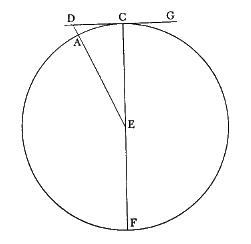
\includegraphics[max width=0.82\textwidth,max height=0.45\textheight,keepaspectratio]{images/figura07.png}\vspace{0.35em}\end{center}


Mi piace a questo punto addurre la causa di un altro fenomeno lunare degno di ammirazione, che, sebbene da me osservato non di recente ma molti anni fa e mostrato, spiegato e chiarito nella sua causa ad alcuni intimi, amici e discepoli, tuttavia, poiché la sua osservazione è resa più semplice e chiara dal telescopio, stimai non inopportuno porre a questo punto, soprattutto perché apparisca più evidente la parentela e similitudine tra la Luna e la Terra.

Mentre la Luna, sia prima che dopo la congiunzione, si trova non lontana dal Sole, il suo globo si offre alla nostra vista non solo dalla parte in cui si orna di corni lucenti ma anche per un breve tratto periferico di tenue chiarore che sembra delineare il contorno della parte tenebrosa, opposta al Sole, e separarla dal campo più oscuro dell'etere stesso. Se con più esatta osservazione consideriamo il fenomeno, vedremo non solo l'estremo lembo della parte tenebrosa rilucere di tale chiarore incerto, ma biancheggiar tutta la faccia della Luna, quella che non ancora riceve i raggi solari, di un certo lume non tanto scarso. Appare tuttavia a un primo sguardo solo un sottile circolo luminoso, per le parti più oscure del cielo che l'attorniano; l'altra superficie sembra invece più oscura per la vicinanza dei corni lucenti che abbagliano la nostra vista. Se però si sceglie un luogo dove da tetto o camino o altro ostacolo posto tra la vista e la Luna (lontano però dall'occhio) siano nascosti i soli corni lucenti, ma l'altra parte del corpo lunare rimanga visibile, si vedrà splendere di non piccolo candore anche questa regione della Luna, quantunque priva della luce solare, soprattutto se già l'oscurità notturna è più profonda per l'assenza del Sole: infatti, in un campo più oscuro la stessa luce appare più chiara. È anche provato che questo secondo (per così dire) candore della Luna è tanto più grande, quanto meno la Luna dista dal Sole: con l'allontanarsi da esso si fa invece sempre minore, finché, dopo la prima quadratura e prima della seconda, si scorge debole e assai incerto, anche se visto in un cielo oscuro: mentre nel sestile e quando la Luna è meno lontana rifulge meravigliosamente, anche nel crepuscolo: rifulge, dico, tanto, che con l'aiuto di un esatto cannocchiale si distinguono in essa le grandi macchie. Questo mirabile candore ha suscitato non piccola meraviglia tra i filosofi; e per mostrarne la causa chi propose una soluzione, chi un'altra. Alcuni lo dissero splendore proprio e naturale della Luna, altri a essa impartito da Venere, altri da tutte le stelle, altri dal Sole, che con i suoi raggi penetrerebbe la solidità della Luna profondamente. Ma invero proposte di tal genere con poca fatica si confutano e si convincono di falsità. Se infatti questa luce fosse propria o apporto delle stelle, la Luna la manterrebbe e mostrerebbe soprattutto nelle eclissi, mentre è posta nel cielo oscurissimo; ma l'esperienza mostra il contrario: infatti il fulgore che appare nella Luna durante le eclissi è assai minore, rossiccio e quasi color bronzo, questo invece è più chiaro e più candido. Inoltre quello è mutevole e mobile di luogo, poiché vaga per la faccia della Luna, così che la parte più vicina alla circonferenza dell'ombra terrestre sempre si vede più chiara, la rimanente più scura: quindi senza alcun dubbio comprendiamo che ciò avviene per la vicinanza dei raggi solari tangenti una qualche regione di più grande densità che avvolge circolarmente la Luna; da questo contatto una specie di aurora si diffonde nelle parti vicine della Luna; non diversamente in Terra all'alba e al tramonto si sparge il lume crepuscolare. Di questo più diffusamente tratteremo nel libro \textit{Del sistema del mondo}. Ed è tanto puerile asserire che quella luce venga da Venere, che non merita confutazione. Infatti chi sarà così ignorante da non comprendere come sia assolutamente impossibile che tra la congiunzione e il sestile la parte della Luna opposta al Sole sia rivolta a Venere? E non si può egualmente ammettere che il fulgore provenga dal Sole che penetri in profondità ed illumini il corpo lunare: infatti questo fulgore non diminuirebbe mai, perché un emisfero della Luna è sempre illuminato dal Sole, eccettuato il tempo delle eclissi lunari; invece diminuisce mentre la Luna si avvia alla quadratura, e del tutto si spegne dopo che l'ha superata. Poiché dunque questo secondo fulgore non è congenito e proprio della Luna, e non è fornito né da stella alcuna né dal Sole, non essendovi più nella vastità dell'universo altro corpo che la Terra, che cosa bisogna concludere, quale soluzione proporre? Non forse che il corpo della Luna, e qualsiasi altro corpo opaco e tenebroso, è illuminato dalla Terra? Che c'è da meravigliarsi? Ecco: giustamente la Terra, grata, rende alla Luna luce pari a quella che essa stessa dalla Luna riceve per quasi tutto il tempo nelle tenebre più profonde della notte. Vediamolo più chiaramente. La Luna nelle congiunzioni, quando si trova tra il Sole e la Terra, è illuminata dai raggi solari nel suo emisfero superiore opposto alla Terra; mentre l'emisfero inferiore che guarda la Terra è avvolto nelle tenebre e perciò non illumina affatto la Terra. La Luna, a poco a poco allontanandosi poi dal Sole e via via illuminandosi in qualche parte dell'emisfero a noi rivolto, ci mostra i corni biancheggianti, ma ancor sottili, e illumina lievemente la Terra; cresce nella Luna, che già s'avvicina alle quadrature, la illuminazione del Sole, aumenta nella Terra il riflettersi della sua luce, si estende per tutto un semicerchio il chiarore della Luna, e le nostre notti splendono più luminose; finalmente tutto l'emisfero lunare a noi rivolto e opposto al Sole è illuminato da fulgidissimi raggi: splende tutta la superficie della Terra perfusa dal chiaro di Luna; poi, decrescente, la Luna manda a noi raggi più deboli, e più debolmente è illuminata la Terra; la Luna si avvia alla congiunzione, oscura notte riempie la Terra. Con tal periodo a vece alterna la Luna ci somministra il chiarore mensile ora più fulgido, ora più debole. Ma con egual misura la Terra ricambia. Infatti, mentre la Luna si trova in congiunzione col Sole ha di fronte tutta la superficie dell'emisfero terrestre esposto al Sole e illuminato vividamente, e riceve la luce riflessa da quella; perciò l'emisfero inferiore della Luna, privo di luce solare, per effetto di tale riflessione appare non poco luminoso. La Luna, allontanatasi di un quadrante dal Sole, vede illuminato solo metà dell'emisfero terrestre, l'occidentale, perché la metà orientale è avvolta da tenebre: perciò la Luna stessa è meno illuminata dalla Terra, e quella sua luce secondaria ci appare più fioca. Se si porrà la Luna in opposizione al Sole, essa vedrà l'emisfero della Terra che è tra lei e il Sole completamente tenebroso e soffuso di oscura notte; se poi tale opposizione sarà eclittica, la Luna non riceverà illuminazione alcuna, priva sia dell'illuminazione del Sole sia di quella della Terra. Nelle sue differenti posizioni fra Terra e Sole, la Luna riceve maggiore o minor lume dalla riflessione della Terra, a seconda che essa guardi una maggiore o minor parte dell'emisfero terrestre illuminato: perché questa relazione è tra i due globi: quando la Terra è maggiormente illuminata dalla Luna, la Luna riceve dalla Terra minor luce e viceversa. Ma questi pochi cenni sull'argomento bastino: se ne parlerà più diffusamente nel nostro \textit{Sistema del mondo}, dove con molteplici ragionamenti ed esperienze si mostrerà validissima la riflessione della luce solare operata dalla Terra a coloro che van dicendo si debba escluderla dal novero degli astri erranti soprattutto perché non ha moto e luce; e dimostreremo che gira e supera lo splendore della Luna, e non è sentina delle terrestri sordidezze e brutture; questo confermeremo con infinite ragioni naturali.

Dicemmo fin qui delle osservazioni fatte sul corpo della Luna: ora parleremo brevemente di quel che intorno alle stelle fisse fu veduto da noi finora. E in primo luogo è degno di attenzione il fatto che le stelle, sia fisse che erranti, quando si guardano con il cannocchiale, non si vedono ingrandite nella proporzione degli altri oggetti e della stessa Luna, ma l'aumento di grandezza per le stelle appare assai minore; così che il cannocchiale capace d'ingrandire gli altri oggetti, per esempio, cento volte, appena lo si crederebbe capace d'ingrandire le stelle quattro o cinque volte. La ragione di questo è nel fatto che gli astri, quando si guardano a occhio nudo, non ci appaiono secondo la lor semplice e nuda (per così dire) grandezza, ma irradiati da certi fulgori e come chiomati da raggi splendenti, soprattutto quando la notte è più fonda; per questo paiono assai maggiori che se fossero privi di quei crini acquisiti: perché l'angolo visuale è determinato non dal vero corpuscolo della stella ma da uno splendore largamente diffuso intorno ad essa. Questo chiarissimamente si può comprendere soprattutto dal fatto che, al cader del Sole, le stelle emergenti nel primo crepuscolo, anche se di prima grandezza, appaiono del tutto esigue; e Venere stessa, quando si offre al nostro sguardo verso il mezzogiorno, risulta così piccola che sembra appena eguagliare una stellina di ultima grandezza. Diversamente accade con altri oggetti e con la stessa Luna, che guardata nella luce meridiana o nelle più fonde tenebre, ci appare sempre di uguale grandezza. In mezzo alle tenebre, dunque, gli astri appaion chiomati, tuttavia la luce diurna può raderli, e non solo questa luce, ma anche una piccola tenue nube che s'interponga tra l'astro e l'occhio che guarda; lo stesso fanno anche veli neri e vetri colorati per l'ostacolo e l'interposizione dei quali le stelle perdono gli splendori circonfusi. Questo egualmente fa il cannocchiale: da prima toglie alle stelle gli splendori acquisiti e accidentali, poi ingrandisce i loro globi semplici (se hanno figura di globi) e le fa apparire ingrandite secondo una minor proporzione, sicché una piccola stella di quinta o sesta grandezza vista al cannocchiale si presenta come di prima grandezza.

Degna di nota sembra anche la differenza tra l'aspetto dei pianeti e quello delle stelle fisse. I pianeti presentano i loro globi esattamente rotondi e definiti e, come piccole lune luminose perfuse ovunque di luce, appaiono circolari: le stelle fisse invece non si vedon mai terminate da un contorno circolare, ma come fulgori vibranti tutt'attorno i loro raggi e molto scintillanti. Si mostrano di uguale figura all'occhio nudo e viste al cannocchiale, ma ingrandite così che una stella di quinta o sesta grandezza sembra eguagliare Canicola, massima delle stelle fisse. Ma oltre le stelle di sesta grandezza si vedrà col cannocchiale un così gran numero di altre, invisibili alla vista naturale, che appena è credibile: se ne possono vedere infatti più di quante ne comprendano le altre sei differenti grandezze; le maggiori di esse, che possiamo chiamare di settima grandezza o prima delle invisibili, con l'aiuto del cannocchiale appaiono più grandi e più luminose che le stelle di seconda grandezza viste a occhio nudo. E perché si abbia prova del loro inimmaginabile numero, volli inserire i disegni di due costellazioni affinché dal loro esempio ci si faccia un'idea delle altre. Nel primo avevo stabilito di raffigurare intera Orione, ma per il grande numero delle stelle e la mancanza di tempo rimandai ad altra occasione questa impresa: ve ne sono infatti, disseminate intorno a quelle già note, entro i limiti di uno o due gradi, più di cinquecento: per questo alle tre già prima note della Cintura e alle sei della Spada ne aggiungemmo ottanta viste di recente; e quanto più esattamente possibile abbiamo conservato le loro distanze: le note e antiche per distinguerle abbiamo disegnato più grandi e contornate da duplice linea; le altre, invisibili, minori e con una linea sola; conservammo anche, come ci fu possibile, le differenze di grandezza.


\begin{center}\vspace{0.6em}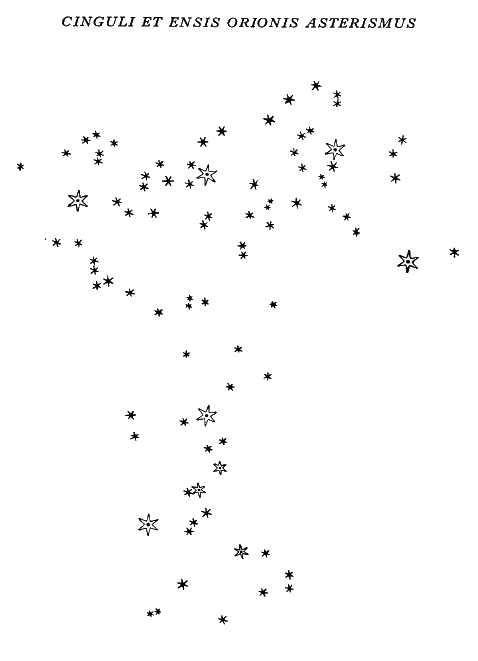
\includegraphics[max width=0.88\textwidth,max height=0.72\textheight,keepaspectratio]{images/figura02.png}\vspace{0.6em}\end{center}


Nel secondo esempio disegnammo sei stelle del Toro dette PLEIADI (dico sei, perché la settima non appare quasi mai), ma chiuse nel cielo entro strettissimi limiti, cui altre invisibili (più di quaranta) sono vicine; delle quali nessuna si allontana più d'un semigrado da una delle sei maggiori: di queste disegnammo soltanto trentasei: e, come per Orione, conservammo le loro distanze, le grandezze, e la distinzione tra vecchie e nuove.

Quello che in terzo luogo osservammo è l'essenza o materia della Via LATTEA, la quale attraverso il cannocchiale si può vedere in modo così palmare che tutte le discussioni, per tanti secoli cruccio dei filosofi, si dissipano con la certezza della sensata esperienza, e noi siamo liberati da sterili dispute. La GALASSIA infatti non è altro che un ammasso di innumerabili stelle disseminate a mucchi; ché in qualunque parte di essa si diriga il cannocchiale, subito si offre alla vista un grandissimo numero di stelle, parecchie delle quali si vedono abbastanza grandi e molto distinte, mentre la moltitudine delle più piccole è affatto inesplorabile.

E poiché non soltanto nella GALASSIA si osserva quel candore latteo come di nube biancheggiante, ma numerose piccole aree di colore consimile splendono qua e là di fioca luce per l'etere, se si volge il cannocchiale in una qualsiasi di quelle ci s'imbatte in un denso ammasso di stelle. E inoltre (meraviglia ancor maggiore) gli astri chiamati finora dagli astronomi NEBULOSE son raggruppamenti di piccole stelle disseminate in modo mirabile: e mentre ciascuna di esse, per la sua piccolezza e cioè per la grandissima distanza da noi, sfugge alla nostra vista, dall'intrecciarsi dei loro raggi risulta quel candore, che finora è stato creduto una parte più densa del cielo, atta a riflettere i raggi delle stelle e del Sole. Noi tra quelle ne osservammo alcune ed abbiam voluto aggiungere i disegni di due.

Nel primo hai una NEBULOSA, chiamata Testa di Orione, nella quale contammo ventuna stelle. Il secondo rappresenta la NEBULOSA chiamata PRESEPE, la quale non è solo una stella, ma una congerie di più che quaranta stelle: noi, oltre gli Asinelli, ne notammo trentasei, disposte nell'ordine seguente.


\begin{center}\vspace{0.6em}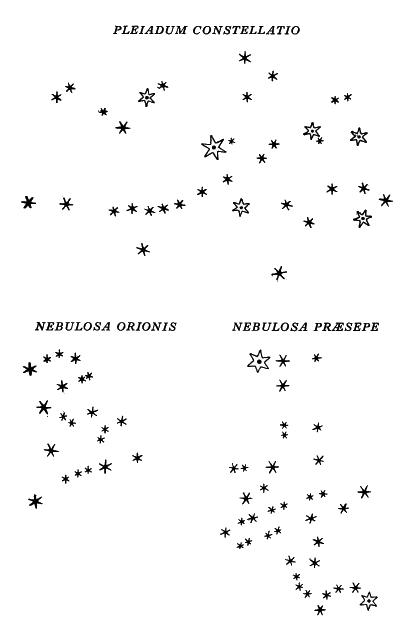
\includegraphics[max width=0.88\textwidth,max height=0.72\textheight,keepaspectratio]{images/figura03.png}\vspace{0.6em}\end{center}


Le cose osservate finora intorno alla Luna, alle stelle fisse, alla Galassia esponemmo brevemente. Resta ora quello che ci sembra l'argomento più importante di questo trattato: e cioè rivelare e divulgare le notizie intorno a quattro PIANETI non mai dal principio del mondo fino ad oggi veduti, l'occasione della scoperta e dello studio, le loro posizioni, e le osservazioni condotte in questi due ultimi mesi sui loro mutamenti e giri, invitando tutti gli astronomi a studiare e definire i loro periodi, cosa che fino ad oggi non ci fu dato fare in alcun modo per ristrettezza di tempo. Ma li avvertiamo che, per non porsi vanamente a questo studio, è necessario il telescopio esattissimo del quale parlammo al principio di questo libro.

Il giorn\textsc{o sette gennaio, d}unque, dell'anno milleseicentodieci, a un'ora di notte, mentre col cannocchiale osservavo gli astri mi si presentò Giove; poiché mi ero preparato uno strumento eccellente, vidi (e ciò prima non mi era accaduto per la debolezza dell'altro strumento) che intorno gli stavano tre stelle piccole ma luminosissime; e quantunque le credessi del numero delle fisse, mi destarono una certa meraviglia, perché apparivano disposte esattamente secondo una linea retta e parallela all'eclittica, e più splendenti delle altre di grandezza uguale alla loro.

Fra loro e rispetto a Giove erano in questo ordine:

\begin{center}\vspace{0.35em}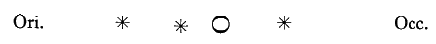
\includegraphics[max width=0.82\textwidth,max height=0.45\textheight,keepaspectratio]{images/figura08.png}\vspace{0.35em}\end{center}
cioè due stelle erano a oriente, una a occidente. La più orientale e l'occidentale apparivano un po' maggiori dell'altra: non mi curai minimamente della loro distanza da Giove, perché, come ho detto, le avevo credute fisse. Quando, non so da qual destino condotto, mi rivolsi di nuovo alla medesima indagine il giorno otto, vidi una disposizione ben diversa: le tre stelle infatti erano tutte a occidente rispetto a Giove, e più vicine tra loro che la notte antecedente e separate da eguali intervalli, come mostra il disegno seguente:

\begin{center}\vspace{0.35em}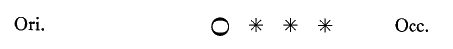
\includegraphics[max width=0.82\textwidth,max height=0.45\textheight,keepaspectratio]{images/figura09.png}\vspace{0.35em}\end{center}
A questo punto, non pensando assolutamente allo spostamento delle stelle, cominciai a chiedermi in qual modo Giove si potesse trovare più ad oriente delle dette stelle fisse, quando il giorno prima era ad occidente rispetto a due di esse. Ed ebbi il dubbio che Giove non fosse per caso diretto, diversamente dal calcolo astronomico, ed avesse col proprio moto oltrepassato quelle stelle. Per questo con gran desiderio aspettai la notte successiva: ma la mia speranza fu resa vana, perché il cielo fu tutto coperto di nubi.

Ma il giorno dieci le stelle mi apparvero in questa posizione rispetto a Giove:

\begin{center}\vspace{0.35em}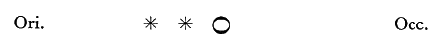
\includegraphics[max width=0.82\textwidth,max height=0.45\textheight,keepaspectratio]{images/figura10.png}\vspace{0.35em}\end{center}
cioè ve n'erano due soltanto, ed entrambe orientali: la terza, come supposi, era nascosta sotto Giove. Erano come prima sulla stessa retta con Giove, e poste esattamente secondo la linea dello Zodiaco. Quando vidi questo e compresi che in alcun modo potevano attribuirsi a Giove simili spostamenti, sapendo inoltre che le stelle osservate eran sempre le stesse (nessun'altra precedente o seguente ve n'era entro grande intervallo sulla linea dello Zodiaco), mutando la perplessità in meraviglia, compresi che l'apparente mutazione non era di Giove ma delle stelle da me scoperte; e per questo pensai di dovere da allora in poi osservare a lungo il fenomeno attentamente e scrupolosamente.

Il giorno undici vidi questa disposizione:

\begin{center}\vspace{0.35em}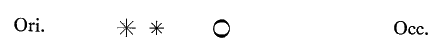
\includegraphics[max width=0.82\textwidth,max height=0.45\textheight,keepaspectratio]{images/figura11.png}\vspace{0.35em}\end{center}
solo due stelle orientali, di cui quella di mezzo distava da Giove il triplo che dalla stella più a oriente: questa era quasi il doppio dell'altra, quantunque la notte antecedente fossero apparse uguali. Stabilii dunque e conclusi fuor d'ogni dubbio che in cielo v'erano stelle vaganti attorno a Giove, come Venere e Mercurio attorno al Sole: cosa che finalmente fu osservata in maniera più chiara alla luce meridiana in numerose altre osservazioni. Fu anche notato che non sono solo tre, ma quattro, le stelle che compiono i loro giri attorno a Giove: la successiva narrazione dirà le lor permutazioni, osservate in seguito più esattamente: misurai anche al telescopio le loro reciproche distanze, nel modo spiegato più sopra: notai pure le ore delle osservazioni, soprattutto quando ne feci molte in una stessa notte: infatti son così veloci le rivoluzioni di questi pianeti che spesso si possono notare differenze anche orarie.

Il giorno dodici, a un'ora di notte, così vidi disposte le stelle:

\begin{center}\vspace{0.35em}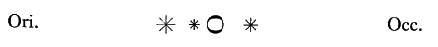
\includegraphics[max width=0.82\textwidth,max height=0.45\textheight,keepaspectratio]{images/figura12.png}\vspace{0.35em}\end{center}
la stella più orientale era maggiore della più occidentale: tuttavia erano entrambe molto visibili e lucenti: l'una e l'altra distavano da Giove due minuti primi. All'ora terza cominciò ad apparire anche una terza stellina, prima non vista, che dalla parte orientale quasi toccava Giove, ed era molto piccola. Tutte erano sulla medesima retta e disposte secondo la linea dell'eclittica.

Il giorno tredici furono da me viste per la prima volta quattro stelle nella seguente posizione rispetto a Giove:

\begin{center}\vspace{0.35em}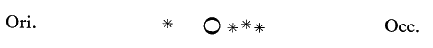
\includegraphics[max width=0.82\textwidth,max height=0.45\textheight,keepaspectratio]{images/figura13.png}\vspace{0.35em}\end{center}
tre erano ad occidente e una ad oriente: formavano all'incirca una linea retta; ché quella che era in mezzo tra le occidentali si scostava di poco dalla retta verso settentrione. La orientale era distante da Giove due minuti, e gli intervalli delle rimanenti e di Giove eran di un sol minuto ciascuno. Tutte le stelle mostravano la stessa grandezza e, benché piccole, erano tuttavia lucentissime e di gran lunga più splendenti delle fisse di egual grandezza.

Il giorno quattordici il tempo fu nuvoloso.

Il quindici, alla terza ora di notte, quattro stelle eran rispetto a Giove nella posizione qui sotto raffigurata:

\begin{center}\vspace{0.35em}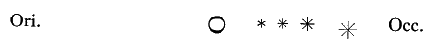
\includegraphics[max width=0.82\textwidth,max height=0.45\textheight,keepaspectratio]{images/figura14.png}\vspace{0.35em}\end{center}
occidentali tutte e disposte quasi su una stessa linea retta; quella che, contando da Giove, era terza, si levava un poco verso borea: la più vicina a Giove era la più piccola, le altre di seguito apparivan maggiori; le distanze fra Giove e le tre stelle seguenti erano uguali tutte e di due minuti, ma la più occidentale distava quattro minuti da quella a lei vicina. Erano alquanto luminose e per nulla scintillanti, quali sempre apparvero, e prima e dopo. All'ora settima c'erano solo tre stelle, e così si vedevano rispetto a Giove:

\begin{center}\vspace{0.35em}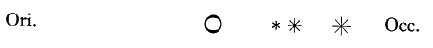
\includegraphics[max width=0.82\textwidth,max height=0.45\textheight,keepaspectratio]{images/figura15.png}\vspace{0.35em}\end{center}
erano cioè esattamente sulla stessa retta: la più vicina a Giove era assai piccola, e lontana da quello tre minuti primi: da questa la seconda distava un minuto: la terza distava dalla seconda 4 minuti e 30 secondi. Dopo un'altra ora le due stelline di mezzo erano ancor più vicine: distavano infatti solo 30 minuti secondi.

Il giorno sedici a un'ora di notte, vidi tre stelle disposte secondo quest'ordine:

\begin{center}\vspace{0.35em}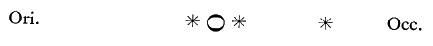
\includegraphics[max width=0.82\textwidth,max height=0.45\textheight,keepaspectratio]{images/figura16.png}\vspace{0.35em}\end{center}
due tenevano in mezzo Giove, distanti da lui zero minuti, 40 secondi da una parte e dall'altra; la terza, occidentale, distava da Giove 8 minuti. Quelle vicine a Giove apparivan non maggiori ma più luminose della più lontana.

Il giorno diciassette, a ore zero e 30 minuti dal tramonto, la configurazione era la seguente:

\begin{center}\vspace{0.35em}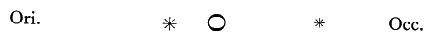
\includegraphics[max width=0.82\textwidth,max height=0.45\textheight,keepaspectratio]{images/figura17.png}\vspace{0.35em}\end{center}
una sola stella orientale distava da Giove 3 minuti; a occidente pure una, che distava da Giove 11 minuti. L'orientale appariva doppia dell'occidentale; non v'erano che queste due. Dopo quattro ore però, cioè verso l'ora quinta, cominciò ad emergerne nella parte orientale una terza che prima, io credo, era in congiunzione con la precedente; tale era la posizione:

\begin{center}\vspace{0.35em}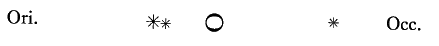
\includegraphics[max width=0.82\textwidth,max height=0.45\textheight,keepaspectratio]{images/figura18.png}\vspace{0.35em}\end{center}
la stella di mezzo, vicinissima all'orientale, si allontanava da quella solo 20 minuti secondi, e declinava un poco verso austro dalla linea retta condotta attraverso le due stelle estreme e Giove.

Il giorno diciotto, a ore zero, 20 minuti dal tramonto, questo era l'aspetto:

\begin{center}\vspace{0.35em}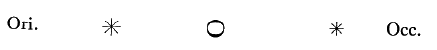
\includegraphics[max width=0.82\textwidth,max height=0.45\textheight,keepaspectratio]{images/figura19.png}\vspace{0.35em}\end{center}
la stella orientale era maggiore dell'occidentale e distante da Giove 8 minuti primi: l'occidentale distava da Giove 10 minuti.

Il giorno diciannove, a due ore di notte, tale era la disposizione delle stelle:

\begin{center}\vspace{0.35em}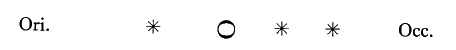
\includegraphics[max width=0.82\textwidth,max height=0.45\textheight,keepaspectratio]{images/figura20.png}\vspace{0.35em}\end{center}
v'erano cioè tre stelle esattamente in linea retta con Giove: una orientale, distante da Giove 6 minuti primi: tra Giove e la prima seguente occidentale c'era una distanza di 5 minuti; questa distava da quella più a occidente 4 minuti. Ero in dubbio se fra la stella orientale e Giove vi fosse una stellina, vicinissima a Giove, tanto che quasi lo toccasse. All'ora quinta però chiaramente la vidi, che già occupava esattamente il punto medio fra Giove e la stella orientale, così che tale era la configurazione:

\begin{center}\vspace{0.35em}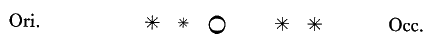
\includegraphics[max width=0.82\textwidth,max height=0.45\textheight,keepaspectratio]{images/figura21.png}\vspace{0.35em}\end{center}
la stella vista per ultima era molto piccola, tuttavia all'ora sesta era quasi uguale in grandezza alle rimanenti.

Il giorno venti, a un'ora, 15 minuti, apparve una consimile disposizione:

\begin{center}\vspace{0.35em}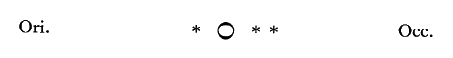
\includegraphics[max width=0.82\textwidth,max height=0.45\textheight,keepaspectratio]{images/figura22.png}\vspace{0.35em}\end{center}
c'eran tre stelle tanto piccole che appena si potevano vedere: da Giove e fra loro non distavano più di un minuto; ero incerto se ad occidente vi fossero due o tre stelline. Circa l'ora sesta erano disposte così:

\begin{center}\vspace{0.35em}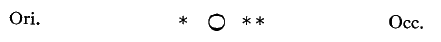
\includegraphics[max width=0.82\textwidth,max height=0.45\textheight,keepaspectratio]{images/figura23.png}\vspace{0.35em}\end{center}
l'orientale distava da Giove il doppio più di prima, cioè 2 minuti; quella di mezzo a occidente distava da Giove zero minuti, 40 secondi, dalla più occidentale zero minuti, 20 secondi. Infine, all'ora settima, si videro a occidente tre stelline:

\begin{center}\vspace{0.35em}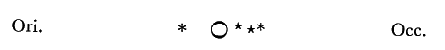
\includegraphics[max width=0.82\textwidth,max height=0.45\textheight,keepaspectratio]{images/figura24.png}\vspace{0.35em}\end{center}
quella più vicina a Giove distava da esso zero minuti, 20 secondi; fra questa e la più occidentale la distanza era di 40 minuti secondi: tra esse se ne vedeva un'altra, volta un po' verso mezzogiorno, lontana da quella più occidentale non più di 10 secondi.

Il giorno ventuno, a ore zero, 30 minuti, v'erano a oriente tre stelline, egualmente distanti fra loro e da Giove:

\begin{center}\vspace{0.35em}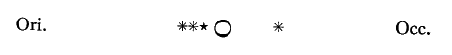
\includegraphics[max width=0.82\textwidth,max height=0.45\textheight,keepaspectratio]{images/figura25.png}\vspace{0.35em}\end{center}
le distanze, secondo stimai, erano di 50 minuti secondi. V'era anche una stella a occidente, distante da Giove 4 minuti primi: l'orientale vicina a Giove era la più piccola; le altre alquanto maggiori, e quasi uguali fra loro.

Il giorno ventidue, alle 2, la disposizione delle stelle era la seguente:

\begin{center}\vspace{0.35em}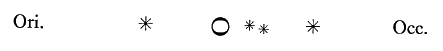
\includegraphics[max width=0.82\textwidth,max height=0.45\textheight,keepaspectratio]{images/figura26.png}\vspace{0.35em}\end{center}
dalla stella orientale a Giove v'era una distanza di 5 minuti primi, da Giove alla più occidentale di 7 primi. Le due stelle occidentali intermedie distavano reciprocamente di zero minuti, 40 secondi; la più vicina a Giove distava da esso un minuto. Le stelline di mezzo eran più piccole di quelle estreme: si estendevano sulla medesima retta secondo la linea dello Zodiaco, se non che quella centrale delle tre occidentali piegava un poco verso austro. Ma, all'ora sesta di notte, apparvero in questa disposizione:

\begin{center}\vspace{0.35em}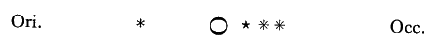
\includegraphics[max width=0.82\textwidth,max height=0.45\textheight,keepaspectratio]{images/figura27.png}\vspace{0.35em}\end{center}
l'orientale era molto piccola, distante da Giove, come prima, 5 minuti. Le tre occidentali distavano egualmente da Giove e fra loro, e le singole distanze erano di circa un minuto, 20 secondi; la stella più vicina a Giove appariva minore delle due seguenti: tutte si vedevano esattamente sulla stessa retta.

Il giorno ventitré, a ore zero, 40 minuti dal tramonto, la disposizione delle stelle era all'incirca questa:

\begin{center}\vspace{0.35em}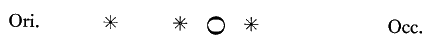
\includegraphics[max width=0.82\textwidth,max height=0.45\textheight,keepaspectratio]{images/figura28.png}\vspace{0.35em}\end{center}
le tre stelle con Giove erano in linea retta secondo la linea dello Zodiaco, come sempre furono; due erano orientali, una occidentale. La più orientale distava dalla successiva 7 minuti primi, questa da Giove 2 minuti, 40 secondi; Giove distava dalla occidentale 3 minuti, 20 secondi; erano tutte quasi eguali per grandezza. Ma all'ora quinta due stelle, che prima eran vicine a Giove, non si vedevano più, nascoste, credo, sotto Giove; e tale era l'aspetto:

\begin{center}\vspace{0.35em}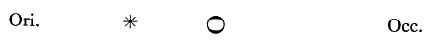
\includegraphics[max width=0.82\textwidth,max height=0.45\textheight,keepaspectratio]{images/figura29.png}\vspace{0.35em}\end{center}
Il giorno ventiquattro si videro tre stelle, orientali tutte e quasi sulla stessa retta con Giove:

\begin{center}\vspace{0.35em}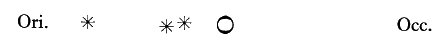
\includegraphics[max width=0.82\textwidth,max height=0.45\textheight,keepaspectratio]{images/figura30.png}\vspace{0.35em}\end{center}
quella di mezzo deviava un po' verso austro. La più vicina a Giove distava da esso 2 minuti, la seguente distava da questa zero minuti, 30 secondi, da questa la più orientale 9 minuti; erano tutte molto splendenti. All'ora sesta solo due si offrivano alla vista, in questa posizione:

\begin{center}\vspace{0.35em}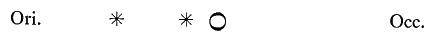
\includegraphics[max width=0.82\textwidth,max height=0.45\textheight,keepaspectratio]{images/figura31.png}\vspace{0.35em}\end{center}
cioè esattamente sulla stessa retta con Giove, da cui la più vicina si allontanava 3 minuti; l'altra distava da questa 8 primi; se non mi inganno le due piccole stelle di mezzo prima osservate s'erano unite in una.

Il giorno venticinque, a un'ora e 40 minuti, così era la disposizione:

\begin{center}\vspace{0.35em}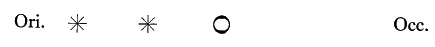
\includegraphics[max width=0.82\textwidth,max height=0.45\textheight,keepaspectratio]{images/figura32.png}\vspace{0.35em}\end{center}
v'erano dunque solo due stelle nella parte orientale, abbastanza grandi: la più orientale distava da quella di mezzo 5 minuti, quella di mezzo da Giove 6 minuti.

Il giorno ventisei, a ore zero, 40 minuti, la collocazione delle stelle era questa:

\begin{center}\vspace{0.35em}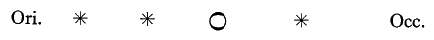
\includegraphics[max width=0.82\textwidth,max height=0.45\textheight,keepaspectratio]{images/figura33.png}\vspace{0.35em}\end{center}
si vedevan dunque tre stelle, delle quali due orientali, la terza occidentale rispetto a Giove: questa distava da esso 5 minuti; la stella centrale a oriente distava da Giove 5 minuti, 20 secondi; la più orientale da quella di mezzo 6 minuti; erano poste sulla stessa retta e di ugual grandezza. All'ora quinta, la disposizione era quasi la stessa, diversa solo pel fatto che a oriente s'affacciava vicino a Giove una quarta stellina, minore delle altre, distante da Giove 30 minuti, ma che si levava un po' dalla linea retta verso borea, come dimostra la figura seguente:

\begin{center}\vspace{0.35em}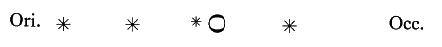
\includegraphics[max width=0.82\textwidth,max height=0.45\textheight,keepaspectratio]{images/figura34.png}\vspace{0.35em}\end{center}
Il giorno ventisette, a un'ora dal tramonto, si vedeva una sola stella, orientale, secondo questa disposizione:

\begin{center}\vspace{0.35em}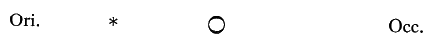
\includegraphics[max width=0.82\textwidth,max height=0.45\textheight,keepaspectratio]{images/figura35.png}\vspace{0.35em}\end{center}
era molto piccola, e lontana da Giove 7 minuti.

Il ventotto e ventinove per l'interporsi di nubi non si poté osservare nulla.

Il giorno trenta, a un'ora di notte, le stelle si vedevano poste così:

\begin{center}\vspace{0.35em}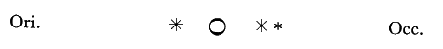
\includegraphics[max width=0.82\textwidth,max height=0.45\textheight,keepaspectratio]{images/figura36.png}\vspace{0.35em}\end{center}
una a oriente, distante da Giove 2 minuti, 30 secondi, due a occidente, di cui la più vicina a Giove distava da esso 3 minuti: l'altra distava da questa un minuto: la posizione delle due stelle estreme e di Giove era sulla medesima retta, ma la stella centrale si levava un po' verso borea: la più occidentale era minore delle altre.

L'ultimo giorno, alle due di notte, si videro due stelle a oriente, una ad occidente:

\begin{center}\vspace{0.35em}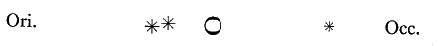
\includegraphics[max width=0.82\textwidth,max height=0.45\textheight,keepaspectratio]{images/figura37.png}\vspace{0.35em}\end{center}
La stella centrale delle due orientali distava da Giove 2 minuti, 20 secondi, la più orientale distava da questa zero minuti, 30 secondi; l'occidentale distava da Giove 10 minuti: erano quasi sulla stessa retta, solo l'orientale più vicina a Giove si levava un poco verso settentrione. All'ora quarta

\begin{center}\vspace{0.35em}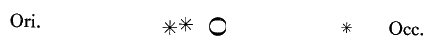
\includegraphics[max width=0.82\textwidth,max height=0.45\textheight,keepaspectratio]{images/figura38.png}\vspace{0.35em}\end{center}
le due orientali erano ancor più vicine fra loro: distavano infatti solo 20 minuti secondi. La stella occidentale apparve in queste osservazioni abbastanza piccola.

Il gior\textsc{no primo febbraio, alla }seconda ora di notte, la posizione era la seguente:

\begin{center}\vspace{0.35em}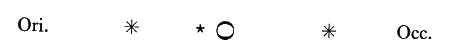
\includegraphics[max width=0.82\textwidth,max height=0.45\textheight,keepaspectratio]{images/figura39.png}\vspace{0.35em}\end{center}
La stella più orientale distava da Giove 6 minuti, la occidentale 8; ad oriente una stella, molto piccola, distava da Giove 20 minuti secondi: determinavano una linea esattamente retta.

Il giorno due le stelle apparvero secondo quest'ordine:

\begin{center}\vspace{0.35em}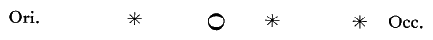
\includegraphics[max width=0.82\textwidth,max height=0.45\textheight,keepaspectratio]{images/figura40.png}\vspace{0.35em}\end{center}
Una sola a oriente, distante da Giove 6 minuti; Giove distava dalla stella occidentale più vicina 4 minuti; fra questa e la più occidentale la distanza era di 8 minuti: erano esattamente sulla stessa retta, e quasi di egual grandezza. Ma, all'ora settima, v'erano quattro stelle:

\begin{center}\vspace{0.35em}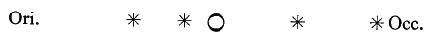
\includegraphics[max width=0.82\textwidth,max height=0.45\textheight,keepaspectratio]{images/figura41.png}\vspace{0.35em}\end{center}
fra le quali Giove occupava il posto di mezzo. Di queste stelle la più orientale distava dalle seguenti 4 minuti, questa da Giove un minuto, 40 secondi: Giove distava dalla stella occidentale più vicina 6 minuti, questa dalla più occidentale 8 minuti: erano ugualmente tutte sulla stessa retta, stesa secondo la linea dello Zodiaco.

Il giorno tre, all'ora settima, le stelle erano disposte in questo ordine:

\begin{center}\vspace{0.35em}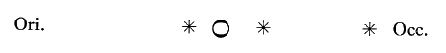
\includegraphics[max width=0.82\textwidth,max height=0.45\textheight,keepaspectratio]{images/figura42.png}\vspace{0.35em}\end{center}
l'orientale distava da Giove un minuto, 30 secondi; l'occidentale vicina 2 minuti: da questa l'altra più occidentale si distanziava di 10 minuti: erano precisamente sulla stessa retta, e di ugual grandezza.

Il giorno quattro, all'ora seconda, stavano attorno a Giove quattro stelle, due orientali e due occidentali, disposte esattamente sulla medesima retta, come nella seguente figura:

\begin{center}\vspace{0.35em}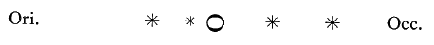
\includegraphics[max width=0.82\textwidth,max height=0.45\textheight,keepaspectratio]{images/figura43.png}\vspace{0.35em}\end{center}
La più orientale distava dalla seguente 3 minuti, questa distava da Giove zero minuti, 40 secondi; Giove distava dalla occidentale vicina 4 minuti, questa dalla più occidentale 6 minuti. Di grandezza erano quasi uguali, la più vicina a Giove appariva un po' minore delle altre. All'ora settima le stelle orientali distavano solo zero minuti, 30 secondi.

\begin{center}\vspace{0.35em}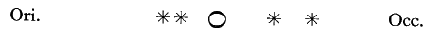
\includegraphics[max width=0.82\textwidth,max height=0.45\textheight,keepaspectratio]{images/figura44.png}\vspace{0.35em}\end{center}
Giove distava dalla orientale più vicina 2 minuti, dalla occidentale seguente 4 minuti; questa distava dalla più occidentale 3 minuti; erano uguali tutte e sulla stessa retta, stesa secondo l'eclittica.

Il giorno cinque il cielo fu nuvoloso.

Il giorno sei apparvero solo due stelle che prendevan Giove nel mezzo, come si vede nella figura seguente:

\begin{center}\vspace{0.35em}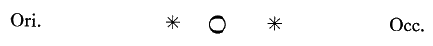
\includegraphics[max width=0.82\textwidth,max height=0.45\textheight,keepaspectratio]{images/figura45.png}\vspace{0.35em}\end{center}
l'orientale distava da Giove 2 minuti, l'occidentale 3 minuti: erano sulla stessa retta con Giove e pari per grandezza.

Il giorno sette v'erano due stelle, entrambe orientali rispetto a Giove, disposte a questo modo:

\begin{center}\vspace{0.35em}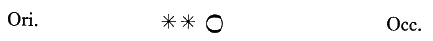
\includegraphics[max width=0.82\textwidth,max height=0.45\textheight,keepaspectratio]{images/figura46.png}\vspace{0.35em}\end{center}
le distanze fra loro e Giove erano uguali, cioè di un minuto primo; fra le stelle e il centro di Giove passava una linea retta.

Il giorno otto, a un'ora, v'erano tre stelle, orientali tutte, come nella figura:

\begin{center}\vspace{0.35em}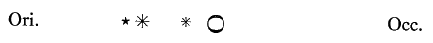
\includegraphics[max width=0.82\textwidth,max height=0.45\textheight,keepaspectratio]{images/figura47.png}\vspace{0.35em}\end{center}
quella vicina a Giove, abbastanza piccola, distava da esso un minuto, 20 secondi; quella di mezzo distava da questa 4 minuti ed era abbastanza grande; la più orientale, molto piccola, distava da questa zero minuti, 20 secondi. Ero incerto se vicino a Giove vi fosse una sola stellina o ve ne fossero due: un'altra si vedeva infatti talvolta esser vicina a questa verso oriente, meravigliosamente piccola, distante dalla prima zero minuti e 10 secondi soltanto: erano tutte sulla stessa linea retta, disposte secondo il corso dello Zodiaco. Alle tre la stella più vicina a Giove quasi lo toccava: ne distava infatti solo zero minuti e 10 secondi: le altre s'eran fatte più lontane da Giove: quella del centro distava infatti da Giove 6 minuti. Infine alle quattro quella ch'era prima la più vicina a Giove, congiunta con esso, non si vedeva più.

Il giorno nove, a ore zero, 30 minuti, stavano presso Giove due stelle a oriente, una ad occidente, in tal disposizione:

\begin{center}\vspace{0.35em}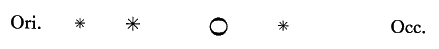
\includegraphics[max width=0.82\textwidth,max height=0.45\textheight,keepaspectratio]{images/figura48.png}\vspace{0.35em}\end{center}
La più orientale, che era abbastanza piccola, distava dalla successiva 4 minuti; quella di mezzo, maggiore, distava da Giove 7 minuti; Giove distava dalla occidentale, che era piccola, 4 minuti.

Il giorno dieci, a un'ora e 30 minuti, due stelline, molto piccole, entrambe orientali, furono viste in tale disposizione:

\begin{center}\vspace{0.35em}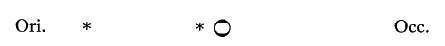
\includegraphics[max width=0.82\textwidth,max height=0.45\textheight,keepaspectratio]{images/figura49.png}\vspace{0.35em}\end{center}
la più lontana distava da Giove 10 minuti, la più vicina zero minuti, 20 secondi; erano sulla stessa retta. Alle quattro però la stella più vicina a Giove non appariva più: anche l'altra si vedeva tanto impiccolita che appena la si poteva distinguere, quantunque l'aria fosse chiarissima, ed era più lontana di prima da Giove, giacché ne distava 12 minuti.

Il giorno undici, a un'ora, v'erano due stelle a oriente, una a occidente. La occidentale distava da Giove 4 minuti, la orientale più vicina

\begin{center}\vspace{0.35em}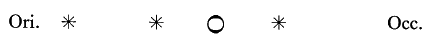
\includegraphics[max width=0.82\textwidth,max height=0.45\textheight,keepaspectratio]{images/figura50.png}\vspace{0.35em}\end{center}
distava ugualmente 4 minuti da Giove; la più orientale distava da questa 8 minuti; erano abbastanza chiare e sulla stessa retta. Ma alle tre una quarta stella, vicinissima a Giove, fu vista ad oriente, minore delle altre, distante da Giove

\begin{center}\vspace{0.35em}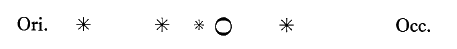
\includegraphics[max width=0.82\textwidth,max height=0.45\textheight,keepaspectratio]{images/figura51.png}\vspace{0.35em}\end{center}
zero minuti, 30 secondi, e deviante un po' verso aquilone dalla linea retta condotta attraverso le altre stelle: erano assai splendenti tutte, e molto visibili. Alle cinque e mezza già la stella orientale più vicina a Giove, fatta da lui più lontana, occupava il posto di mezzo fra Giove e la stella più orientale a lei vicina; erano tutte esattamente sulla stessa linea retta, di pari grandezza, come si può vedere dalla figura seguente:

\begin{center}\vspace{0.35em}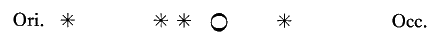
\includegraphics[max width=0.82\textwidth,max height=0.45\textheight,keepaspectratio]{images/figura52.png}\vspace{0.35em}\end{center}
Il giorno dodici, a ore zero, 40 minuti, c'erano due stelle ad oriente, due parimenti ad occidente. La orientale più lontana distava da Giove 10 minuti, l'occidentale più lontana 8,

\begin{center}\vspace{0.35em}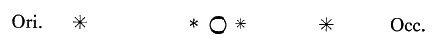
\includegraphics[max width=0.82\textwidth,max height=0.45\textheight,keepaspectratio]{images/figura53.png}\vspace{0.35em}\end{center}
ed erano entrambe abbastanza visibili; le altre due erano vicinissime a Giove, e molto piccole, soprattutto quella ad oriente che distava da Giove zero minuti, 40 secondi; l'occidentale ne distava un minuto. Alle quattro la stellina che era più vicina a Giove ad oriente, non appariva più.

Il giorno tredici, a ore zero, 30 minuti, apparivano due stelle ad oriente, due ad occidente.

\begin{center}\vspace{0.35em}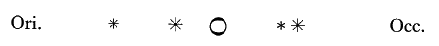
\includegraphics[max width=0.82\textwidth,max height=0.45\textheight,keepaspectratio]{images/figura54.png}\vspace{0.35em}\end{center}
L'orientale più vicina a Giove, abbastanza chiara, distava da esso 2 minuti; da questa la più orientale, meno visibile, distava 4 minuti. Fra le occidentali, la più lontana da Giove, meno visibile, se ne allontanava 4 minuti; fra questa e Giove si interponeva una piccola stella più vicina alla stella più occidentale, distando da quella non più di zero minuti, 30 secondi. Erano tutte sulla stessa retta, esattamente secondo la linea dell'eclittica.

Il giorno quindici (il quattordici il cielo era stato coperto da nubi), a un'ora, tale era la posizione degli astri:

\begin{center}\vspace{0.35em}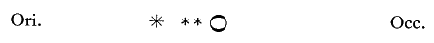
\includegraphics[max width=0.82\textwidth,max height=0.45\textheight,keepaspectratio]{images/figura55.png}\vspace{0.35em}\end{center}
v'erano cioè tre stelle a oriente, e nessuna se ne vedeva a occidente: l'orientale più vicina a Giove ne distava zero minuti, 50 secondi; la successiva distava da questa zero minuti, 20 secondi; da questa ultima la più orientale distava 2 minuti, ed era maggiore delle altre; le più vicine a Giove erano infatti molto piccole. Ma, verso le cinque, delle stelle vicine a Giove se ne vedeva solo una,

\begin{center}\vspace{0.35em}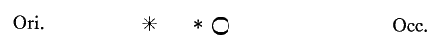
\includegraphics[max width=0.82\textwidth,max height=0.45\textheight,keepaspectratio]{images/figura56.png}\vspace{0.35em}\end{center}
distante da esso zero minuti, 30 secondi; la distanza da Giove della più orientale era aumentata: era infatti allora di 4 minuti. Ma, alle sei, oltre le due, come ora si disse, poste ad oriente, si vedeva verso occidente una stellina, molto piccola, distante da Giove 2 minuti.

\begin{center}\vspace{0.35em}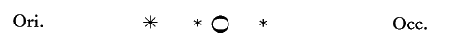
\includegraphics[max width=0.82\textwidth,max height=0.45\textheight,keepaspectratio]{images/figura57.png}\vspace{0.35em}\end{center}
Il giorno sedici, alle sei, erano in tale posizione:

\begin{center}\vspace{0.35em}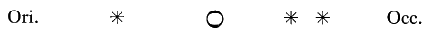
\includegraphics[max width=0.82\textwidth,max height=0.45\textheight,keepaspectratio]{images/figura58.png}\vspace{0.35em}\end{center}
la stella orientale distava da Giove 7 minuti, Giove da quella che lo seguiva a occidente 5 minuti, questa dalla restante più occidentale 3 minuti: erano tutte quasi di ugual grandezza, abbastanza visibili, e sulla stessa linea retta, esattamente secondo il cammino dello Zodiaco.

Il giorno diciassette, a un'ora, c'erano due stelle:

\begin{center}\vspace{0.35em}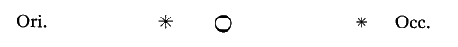
\includegraphics[max width=0.82\textwidth,max height=0.45\textheight,keepaspectratio]{images/figura59.png}\vspace{0.35em}\end{center}
orientale una, distante da Giove 3 minuti, occidentale l'altra, distante 10 minuti: questa era alquanto minore della orientale. Ma, alle sei, la orientale era più vicina a Giove, perché distava zero minuti, 50 secondi; la occidentale invece era più lontana, cioè 12 minuti. In entrambe le osservazioni erano sulla stessa retta, ed entrambe abbastanza piccole, soprattutto la orientale nella seconda osservazione.

Il giorno 18, a un'ora, c'erano tre stelle, delle quali due occidentali, una orientale: la orientale distava da Giove 3 minuti, l'occidentale più vicina 2 minuti;

\begin{center}\vspace{0.35em}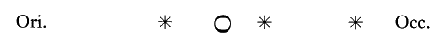
\includegraphics[max width=0.82\textwidth,max height=0.45\textheight,keepaspectratio]{images/figura60.png}\vspace{0.35em}\end{center}
la più occidentale distava da quella di mezzo 8 minuti: tutte erano esattamente sulla stessa retta, e quasi di pari grandezza. Ma, alle due, le stelle più vicine distavan da Giove per intervalli uguali: l'occidentale infatti ne distava anch'essa 3 minuti. Alle sei però si vide una quarta stellina fra la più orientale e Giove, in tal disposizione:

\begin{center}\vspace{0.35em}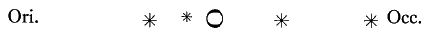
\includegraphics[max width=0.82\textwidth,max height=0.45\textheight,keepaspectratio]{images/figura61.png}\vspace{0.35em}\end{center}
la più orientale distava dalla seguente 3 minuti, la seguente da Giove un minuto, 50 secondi, Giove distava dalla occidentale che lo seguiva 3 minuti, questa dalla più occidentale 7 minuti: erano quasi uguali, solo la orientale vicina a Giove era un po' più piccola delle altre: erano sulla stessa retta, parallela all'eclittica.

Il giorno 19, a ore zero, 40 minuti, si videro solo due stelle, occidentali rispetto a Giove

\begin{center}\vspace{0.35em}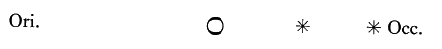
\includegraphics[max width=0.82\textwidth,max height=0.45\textheight,keepaspectratio]{images/figura62.png}\vspace{0.35em}\end{center}
abbastanza grandi ed esattamente sulla stessa retta con Giove, disposte secondo il cammino dell'eclittica. La più vicina distava da Giove 7 minuti, questa dalla più occidentale 6 minuti.

Il giorno 20 il cielo fu nuvoloso.

Il giorno 21, a un'ora, 30 minuti, si vedevano tre stelline abbastanza piccole, in questa disposizione:

\begin{center}\vspace{0.35em}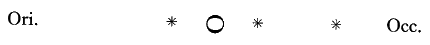
\includegraphics[max width=0.82\textwidth,max height=0.45\textheight,keepaspectratio]{images/figura63.png}\vspace{0.35em}\end{center}
l'orientale distava da Giove 2 minuti, Giove dalla occidentale che seguiva 3 minuti, questa 7 minuti dalla più occidentale: erano esattamente sulla stessa linea parallela all'eclittica.

Il giorno 25, a un'ora, 30 minuti (nelle tre notti precedenti il cielo era stato coperto di nubi) apparvero tre stelle:

\begin{center}\vspace{0.35em}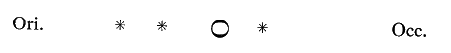
\includegraphics[max width=0.82\textwidth,max height=0.45\textheight,keepaspectratio]{images/figura64.png}\vspace{0.35em}\end{center}
due orientali, le cui distanze reciproche e da Giove erano uguali, di 4 minuti; a occidente una distava da Giove 2 minuti: erano esattamente sulla stessa retta, secondo il cammino dell'eclittica.

\textsc{Il giorno 26, a} ore zero, 30 minuti, v'erano soltanto due stelle:

\begin{center}\vspace{0.35em}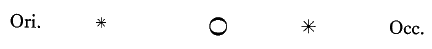
\includegraphics[max width=0.82\textwidth,max height=0.45\textheight,keepaspectratio]{images/figura65.png}\vspace{0.35em}\end{center}
una orientale, distante da Giove 10 minuti, l'altra occidentale, distante 6 minuti: l'orientale era alquanto minore dell'occidentale. Ma alle 5 si videro tre stelle:

\begin{center}\vspace{0.35em}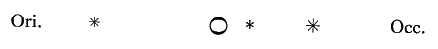
\includegraphics[max width=0.82\textwidth,max height=0.45\textheight,keepaspectratio]{images/figura66.png}\vspace{0.35em}\end{center}
oltre le due già segnalate se ne vedeva una terza a occidente, presso Giove, molto piccola, che prima era nascosta sotto Giove, e ne distava un minuto; la stella orientale appariva più lontana di prima, distando da Giove 11 minuti. Questa notte mi piacque osservare per la prima volta il cammino di Giove e dei pianeti vicini, secondo la linea dello Zodiaco, in relazione ad una stella fissa: si vedeva infatti u\textsc{na stella fissa verso oriente, d}istante dal pianeta orientale 11 minuti, e poco volgeva verso austro, nel modo che segue:

\begin{center}\vspace{0.35em}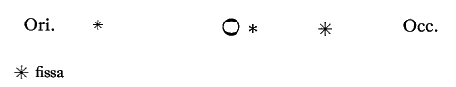
\includegraphics[max width=0.82\textwidth,max height=0.45\textheight,keepaspectratio]{images/figura67.png}\vspace{0.35em}\end{center}
Il giorno 27, a un'ora, 4 minuti, le stelle apparivano in tale configurazione:

\begin{center}\vspace{0.35em}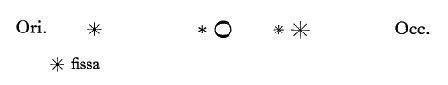
\includegraphics[max width=0.82\textwidth,max height=0.45\textheight,keepaspectratio]{images/figura68.png}\vspace{0.35em}\end{center}
la più orientale distava da Giove 10 minuti, la seguente, vicina a Giove, zero minuti, 30 secondi; l'occidentale che seguiva distava 2 minuti, 30 secondi; da questa la più occidentale distava un minuto. Le più vicine a Giove apparivano piccole, soprattutto l'orientale; le estreme invece erano molto visibili, particolarmente quella a occidente; designavano esattamente una linea retta secondo il cammino dell'eclittica. Il cammino di questi pianeti verso oriente si vedeva chiaramente dal riferimento alla predetta stella fissa; ad essa infatti Giove con i pianeti adiacenti era più vicino, come si può vedere nella figura. Ma alle 5 la stella orientale prossima a Giove ne distava un minuto.

Il giorno 28, a un'ora, si vedevano solo due stelle; una orientale, distante da Giove 9 minuti, una occidentale, distante 2 minuti: erano abbastanza visibili e sulla stessa retta: la stella fissa, perpendicolarmente a questa linea, cadeva sul pianeta orientale, come nella figura:

\begin{center}\vspace{0.35em}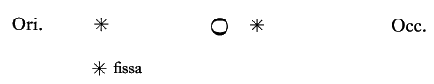
\includegraphics[max width=0.82\textwidth,max height=0.45\textheight,keepaspectratio]{images/figura69.png}\vspace{0.35em}\end{center}
ma, alle 5, fu vista una terza stellina, distante ad oriente da Giove 2 minuti, in questa posizione:

\begin{center}\vspace{0.35em}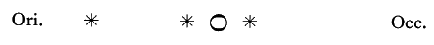
\includegraphics[max width=0.82\textwidth,max height=0.45\textheight,keepaspectratio]{images/figura70.png}\vspace{0.35em}\end{center}
Il giorno primo di marzo, a ore zero, 40 minuti, furono viste quattro stelle, tutte orientali, di cui la più vicina a Giove distava da esso 2 minuti; la successiva distava da questa un minuto, la terza zero minuti, 2 secondi, ed era più luminosa delle altre: da questa la più orientale distava 4 minuti, ed era più piccola delle rimanenti. Segnavano una linea quasi retta, se non che la terza a contar da Giove era un po' sollevata. La stella fissa formava con Giove e la stella più orientale un triangolo equilatero, come nella figura:

\begin{center}\vspace{0.35em}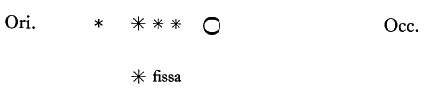
\includegraphics[max width=0.82\textwidth,max height=0.45\textheight,keepaspectratio]{images/figura71.png}\vspace{0.35em}\end{center}
Il giorno 2, a zero ore, 40 minuti, c'erano tre pianeti, due orientali, uno occidentale, in tale configurazione:

\begin{center}\vspace{0.35em}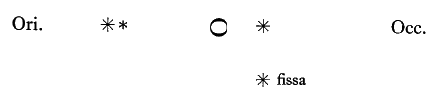
\includegraphics[max width=0.82\textwidth,max height=0.45\textheight,keepaspectratio]{images/figura72.png}\vspace{0.35em}\end{center}
Il più orientale distava da Giove 7 minuti, da questo il seguente zero minuti, 30 secondi; l'occidentale si allontanava da Giove 2 minuti; gli estremi erano più luminosi e più grandi dell'altro, che appariva molto piccolo. Il più orientale sembrava un po' elevato verso borea dalla linea retta condotta attraverso i restanti pianeti e Giove. La stella fissa già notata distava 8 minuti dal pianeta occidentale, secondo la perpendicolare condotta dal pianeta stesso sulla retta passante per tutti i pianeti, come dimostra la figura annessa.

Mi piacque aggiungere questi confronti di Giove e i pianeti vicini con la stella fissa, affinché da quelli chiunque possa intendere che i movimenti dei pianeti medesimi, sia secondo la longitudine che secondo la latitudine, concordano minutamente con i moti che si traggono dalle tavole.

Queste sono le osservazioni sui quattro Astri Medicei di recente per la prima volta da me scoperti, dalle quali pur non essendo ancora possibile addurre i loro periodi, è lecito dir cose degne di attenzione. In primo luogo, poiché ora seguono, ora precedono Giove ad uguali intervalli e si allontanano da esso solo ben poco spazio ora verso oriente ora verso occidente, e lo accompagnano sia nel moto retrogrado che nel diretto, a nessuno può nascer dubbio che compiano attorno a Giove le loro rivoluzioni, e nello stesso tempo effettuino tutti insieme con periodo dodecennale il lor giro intorno al centro del mondo. Inoltre si volgono in orbite ineguali come manifestamente si comprende dal fatto che nei momenti di massima digressione da Giove non si possono mai vedere due pianeti congiunti, mentre vicino a Giove se ne trovano riuniti due, tre ed a volte tutti insieme. Si nota ancora che sono più veloci le rivoluzioni dei pianeti i quali descrivono intorno a Giove orbite minori: infatti le stelle più vicine a Giove spesso si vedono orientali mentre il giorno prima erano apparse occidentali, e viceversa: ma il pianeta che descrive l'orbita maggiore, ad un accurato esame delle predette rivoluzioni mostra aver periodo semimensile. Abbiamo dunque un valido ed eccellente argomento per togliere ogni dubbio a coloro che, accettando tranquillamente nel sistema di Copernico la rivoluzione dei pianeti intorno al Sole, sono tanto turbati dal moto della sola Luna intorno alla Terra, mentre entrambi compiono ogni anno la loro rivoluzione attorno al Sole, da ritenere si debba rigettare come impossibile questa struttura dell'universo. Ora, infatti, non abbiamo un solo pianeta che gira intorno a un altro, mentre entrambi percorrono la grande orbita intorno al Sole, ma la sensata esperienza ci mostra quattro stelle erranti attorno a Giove, così come la Luna attorno alla Terra, mentre tutte insieme con Giove, con periodo di dodici anni si volgono in ampia orbita attorno al Sole. E finalmente non bisogna tacere per quale ragione accada che gli Astri Medicei, mentre compiono attorno a Giove piccolissime rivoluzioni, sembrano talvolta più grandi del doppio. Non possiamo ricercarne la causa nei vapori terrestri, perché appaiono più grandi e più piccoli, mentre Giove e le vicine stelle fisse si vedono immutate. Sembra anche del tutto impossibile che quelle si allontanino tanto dalla Terra nel loro apogeo e tanto le si avvicinino nel loro perigeo da essere questa l'origine di così grande cambiamento. Infatti una stretta rotazione circolare non può in alcun modo produrre simile effetto; ed un moto ovale (che in questo caso sarebbe quasi retto) sembra impensabile e per nulla consono a quanto si osserva. Le soluzioni che a questo proposito mi si presentano alla mente, volentieri espongo, e le offro al giudizio e alla critica dei filosofi. Si sa che per l'interposizione dei vapori terrestri il Sole e la Luna appaiono maggiori, minori invece le stelle fisse e i pianeti: quindi i due luminari vicino all'orizzonte appaion più grandi, mentre le stelle, più piccole e spesso a pena visibili, diminuiscono ancor più se quei vapori vengono illuminati; per questo le stelle durante il giorno e nei crepuscoli appaiono assai fioche, non così la Luna, come sopra avvertimmo. E che non solo la Terra ma anche la Luna sia circondata da vapori, risulta sia da quanto dicemmo sopra, sia da quello che più diffusamente diremo nel nostro \textit{Sistema}. Possiamo dunque a ragione credere la stessa cosa per gli altri pianeti, e non sembra assolutamente improbabile che vi sia un involucro più denso del rimanente etere anche attorno a Giove, intorno al quale, come la Luna attorno alla sfera degli elementi, girano i Pianeti Medicei e, con l'interposizione di questo involucro più denso, all'apogeo sembran minori, mentre al perigeo maggiori per la mancanza o almeno l'attenuarsi dell'involucro stesso. La ristrettezza del tempo ci impedisce di andare oltre: il benigno lettore aspetti fra breve una più ampia trattazione di questo argomento.

% =========================================================================
% PARTE SECONDA: TESTO ORIGINALE LATINO (SIDEREUS NUNCIUS)
% =========================================================================
\begin{otherlanguage}{latin}
\part*{Pars Secunda\\{\Large\scshape\color{rubric} Sidereus Nuncius}\\{\normalsize\itshape Testo originale latino (Venetiis, MDCX)}}
\addcontentsline{toc}{part}{Pars Secunda: Sidereus Nuncius (Testo originale latino)}

\chapter*{Serenissimo Cosmo Medices II Magno Etruriae Duci IIII}
\addcontentsline{toc}{chapter}{Serenissimo Cosmo Medices II Magno Etruriae Duci IIII}

Præclarum sane atque humanitatis plenum eorum fuit institutum, qui excellentium virtute virorum res præclare gestas ab invidia tutari, eorumque immortalitate digna nomina ab oblivione atque interitu vindicare, conati sunt. Hinc ad memoriam posteritatis proditæ imagines, vel marmore insculptæ, vel ex ære fictæ; hinc positæ statuæ, tam pedestres, quam equestres; hinc columnarum atque pyramidum, ut inquit ille,\textsc{ }sumptus ad sidera ducti; hinc denique urbes ædificatæ, eorumque insignitæ nominibus, quos grata posteritas æternitati commendandos existimavit. Eiusmodi est enim humanæ mentis conditio, ut nisi assiduis rerum simulacris in eam extrinsecus irrumpentibus pulsetur, omnis ex illa recordatio facile effluat.

Verum alii firmiora ac diuturniora spectantes, æternum summorum virorum præconium non saxis ac metallis, sed Musarum custodiæ et incorruptis litterarum monumentis consecrarunt. At quid ego ista commemoro? quasi vero humana solertia, his contenta regionibus, ulterius progredi non sit ausa; attamen longius illa prospiciens, cum optime intelligeret, omnia humana monumenta vi tempestate ac vetustate tandem interire, incorruptiora signa excogitavit, in quæ tempus edax atque invidiosa vetustas nullum sibi ius vindicaret. In cælum itaque migrans, clarissimorum Siderum notis sempiternis illis Orbibus eorum nomina consignavit, qui ob egregia ac prope divina facinora digni habiti sunt, qui una cum Astris ævo sempiterno fruerentur. Quam ob rem non prius Iovis, Martis, Mercurii, Herculis cæterorumque heroum, quorum nominibus Stellæ appellantur, fama obscurabitur, quam ipsorum Siderum splendor extinguatur. Hoc autem humanæ sagacitatis inventum, cum primis nobile ac mirandum, multorum iam sæculorum intervallo exolevit, priscis heroibus lucidas illas sedes occupantibus ac suo quasi iure tenentibus: in quorum cœtum frustra pietas Augusti Iulium Cæsarem cooptare conata est; nam cum Stellam suo tempore exortam, ex iis quas Græci Cometas, nostri Crinitas vocant, Iulium Sidus nuncupari voluisset, brevi illa evanescens, tantæ cupiditatis spem delusit. Atqui longe veriora ac feliciora, Princeps Serenissime, Celsitudini tuæ possumus augurari; nam vix dum in terris immortalia animi tui decora fulgere cœperunt, cum in Cælis lucida Sidera sese offerunt, quæ tanquam linguæ prestantissimas virtutes tuas in omne tempus loquantur ac celebrent. En igitur quatuor Sidera tuo inclyto nomini reservata, neque illa de gregario ac minus insigni inerrantium numero, sed ex illustri vagantium ordine; quæ quidem disparibus inter se motibus circum Iovis Stellam cæterarum nobilissimam, tanquam germana eius progenies, cursus suos orbesque conficiunt celeritate mirabili, interea dum unanimi concordia circa mundi centrum, circa Solem\textsc{ }nempe ipsum, omnia simul duodecimo\textsc{ }quoque anno magnas convolutiones absolvunt. Ut autem inclito Celsitudinis tuæ nomini præ ceteris novos hosce Planetas destinarem, ipsemet Siderum Opifex perspicuis argumentis me admonere visus est. Etenim, quemadmodum hæ Stellæ, tanquam Iove digna proles, nunquam ab illius latere, nisi exiguo intervallo, discedunt; ita quis ignorat clementiam, animi mansuetudinem, morum suavitatem, regii sanguinis splendorem, in actionibus maiestatem, auctoritatis et Imperii in alios amplitudinem, quæ quidem omnia in tua Celsitudine sibi domicilium ac sedem collocarunt, quis, inquam, ignorat, hæc omnia ex benignissimo Iovis astro, secundum Deum omnium bonorum fontem, emanare? Iuppiter,\textsc{ }Iuppiter, inquam, a primo Celsitudinis tuæ ortu, turbidos horizontis vapores iam transgressus, mediumque cæli cardinem occupans, orientalemque angulum sua regia illustrans, felicissimum partum ex sublimi illo throno prospexit, omnemque splendorem atque amplitudinem suam in purissimum aërem profudit, ut universam illam vim ac potestatem tenerum corpusculum una cum animo, nobilioribus ornamentis iam a Deo decorato, primo spiritu hauriret. Verum, quid ego probabilibus utor argumentationibus, cum id necessaria propemodum ratione concludere ac demonstrare queam? Placuit Deo Optimo Maximo, ut a Serenissimis parentibus tuis non indignus existimarer, qui Celsitudini tuæ in tradendis Mathematicis disciplinis operam navarem; quod quidem præstiti quatuor superioribus annis proxime elapsis, eo anni tempore, quo a severioribus studiis ocium esse consuevit. Quo circa cum mihi divinitus plane contigerit, ut Celsitudini tuæ inservirem, atque ideo incredibilis clementiæ ac benignitatis tuæ radios propius exceperim, quid mirum si animus meus adeo incaluit, ut nihil aliud propemodum dies noctesque meditetur, quam ut ego, qui non solum animo, sed etiam ipso ortu ac natura, sub tua dominatione sum, tuæ gloriæ cupidissimus et quam gratissimus erga te esse cognoscar? Quæ cum ita sint, cum, te Auspice, COSME Serenissime, has Stellas superioribus Astronomis omnibus incognitas exploraverim, optimo iure eas Augustissimo Prosapiæ tuæ nomine insignire decrevi. Quod si illas primus indagavi, quis me iure reprehendat, si iisdem quoque nomen imposuero, ac MEDICEA SIDERA appellaro? sperans fore, ut tantum dignitatis ex hac appellatione iis Sideribus accedat, quantum alia cæteris Heroibus attulerunt. Nam, ut taceam de Serenissimis tuis Maioribus, quorum gloriam sempiternam omnium historiarum monumenta testantur, sola tua virtus, Maxime Heros, illis Astris impertiri potest nominis immortalitatem. Cui enim dubium esse potest, quin, quam tui expectationem felicissimis imperii auspiciis concitasti, quamvis summam, eam non solum sustineas ac tuearis, verum etiam longo intervallo superaturus sis? ut cum alios tui similes viceris, tecum nihilominus ipse certes, ac te ipso ac magnitudine tua in dies maior evadas.

Suscipe itaque, Clementissime Princeps, hanc tibi ab Astris reservatam gentiliciam gloriam, et illis divinis bonis, quæ non tam a Stellis, quam a Stellarum Opifice ac Moderatore Deo, tibi deferuntur, quam diutissime fruere.

Datum Patavii, 4 Idus Martii, MDCX.

Celsitudinis tuæ

Addictissimus Servus

Galileus Galileus.

\chapter*{Licentia Capitum Excelsi Consilii Decem}
\addcontentsline{toc}{chapter}{Licentia Capitum Excelsi Consilii Decem}

Gli Eccellentissimi Signori Capi dell'Ecc. Cons. de' X infrascritti, avuta fede dalli Signori Reformatori del Studio di Padova per relazione delli due a questo deputati, cioè dal Rever. P. Inquisitor, e dal circospetto Secretario del Senato, Gio. Maraviglia, con giuramento, come nel libro intitolato: SIDEREUS NUNCIUS etc. di D. Galileo Galilei non si trova alcuna cosa contraria alla Santa Fede Cattolica, Prencipi e buoni costumi, e che è degno di stampa, concedono licenza che possi esser stampato in questa Città.

Datum die primo Martii 1610.

\begin{center}
$\left.\begin{tabular}{@{}l@{}}
D. M. Ant. Valaresso \\
D. Nicolò Bon \\
D. Lunardo Marcello
\end{tabular}\right\}$ \textit{Capi dell'Ecc. Cons. de' X}
\end{center}

Illustrissimi Consilii X Secretarius

Bartholomæs Cominus.

1610, a dì 8 Marzo. Regist. in libro a car. 39.

Ioan. Baptista Breatto off.

Con. Blasph. Coad.

\chapter{Astronomicus Nuncius}
\begin{center}
{\itshape Observationes recens habitae beneficio perspicilli in Lunae facie, Lacteo Circulo Stelliisque nebulosis, Innumeris Fixis, necnon in quatuor Planetis Medicea Sidera nuncupatis, nunquam in hanc usque diem cognitis\par}
\end{center}
\bigskip

Magna equidem in hac exigua tractatione singulis de natura speculantibus inspicienda contemplandaque propono. Magna, inquam, tum ob rei ipsius præstantiam, tum ob inauditam per ævum novitatem, tum etiam propter Organum, cuius beneficio eadem sensui nostro obviam sese fecerunt.

Magnum sane est, supra numerosam inerrantium Stellarum multitudinem, quæ naturali facultate in hunc usque diem conspici potuerunt, alias innumeras superaddere oculisque palam exponere, antehac conspectas nunquam, et quæ veteres ac notas plusquam supra decuplam multiplicitatem superent.

Pulcherrimum atque visu iucundissimum est, lunare corpus, per sex denas fere terrestres semidiametros\textsc{ }a nobis remotum, tam ex propinquo intueri, ac si per duas tantum easdem dimensiones distaret; adeo ut eiusdem Lunæ diameter vicibus quasi terdenis, superficies vero noningentis, solidum autem corpus vicibus proxime viginti septem millibus, maius appareat, quam dum libera tantum oculorum acie spectatur: ex quo deinde sensata certitudine quispiam intelligat, Lunam superficie leni et perpolita nequaquam esse indutam, sed aspera et inæquali; ac, veluti ipsiusmet Telluris facies, ingentibus tumoribus, profundis lacunis atque anfractibus undiquaque confertam existere.

Altercationes insuper de Galaxia, seu de Lacteo circulo, substulisse, eiusque essentiam sensui, nedum intellectui, manifestasse, parvi momenti existimandum minime videtur; insuperque substantiam Stellarum, quas Nebulosas hucusque Astronomorum quilibet appellavit, digito demonstrare, longeque aliam esse quam creditum hactenus est, iocundum erit atque perpulcrum.

Verum, quod omnem admirationem longe superat, quodve admonitos faciendos cunctos Astronomos atque Philosophos nos apprime impulit, illud est, quod scilicet quatuor Erraticas Stellas, nemini eorum qui ante nos cognitas aut observatas, adinvenimus, quæ circa Stellam quandam insignem e numero cognitarum, instar Veneris atque Mercurii circa Solem, suas habent periodos, eamque modo præeunt, modo subsequuntur, nunquam extra certos limites ab illa digredientes. Quæ omnia ope Perspicilli a me excogitati, divina prius illuminante gratia, paucis abhinc diebus, reperta atque observata fuerunt.

Alia forte præstantiora, vel a me, vel ab aliis, in dies adinvenientur consimilis Organi beneficio; cuius formam et apparatum, necnon illius excogitandi occasionem, prius breviter commemorabo, deinde habitarum a me observationum historiam recensebo.

Mensibus abhinc decem fere, rumor ad aures nostras increpuit, fuisse a quodam Belga Perspicillum elaboratum, cuius beneficio obiecta visibilia, licet ab oculo inspicientis longe dissita, veluti propinqua distincte cernebantur; ac huius profecto admirabilis effectus nonnullæ experientiæ circumferebantur, quibus fidem alii præbebant, negabant alii. Idem paucos post dies mihi per literas a nobili Gallo Iacobo Badovere\textsc{ }ex Lutetia confirmatum est; quod tandem in causa fuit, ut ad rationes inquirendas, necnon media excogitanda, per quæ ad consimilis Organi inventionem devenirem, me totum converterem; quam paulo post, doctrinæ de refractionibus innixus, assequutus sum: ac tubum primo plumbeum mihi paravi, in cuius extremitatibus vitrea duo Perspicilla, ambo ex altera parte plana, ex altera vero unum sphærice convexum, alterum vero cavum aptavi; oculum deinde ad cavum admovens obiecta satis magna et propinqua intuitus sum; triplo enim viciniora, nonuplo vero maiora apparebant, quam dum sola naturali acie spectarentur. Alium postmodum exactiorem mihi elaboravi, qui obiecta plusquam sexagesies maiora repræsentabat. Tandem, labori nullo nullisque sumptibus parcens, eo a me deventum est, ut Organum mihi construxerim adeo excellens, ut res per ipsum visæ millies fere maiores appareant, ac plusquam in terdecupla ratione viciniores, quam si naturali tantum facultate spectentur. Huius Instrumenti quot quantaque sint commoda, tam in re terrestri quam in maritima, omnino supervacaneum foret enumerare. Sed, missis terrenis, ad Cælestium speculationes me contuli; ac Lunam prius tam ex propinquo sum intuitus, ac si vix per duas Telluris diametros\textsc{ }abesset. Post hanc, Stellas tum fixas, tum vagas,\textsc{ }incredibili animi iucunditate sæpius observavi; cumque harum maximam frequentiam viderem, de ratione, qua illarum interstitia dimetiri possem, excogitare cœpi, ac demum reperi. Qua de re singulos præmonitos esse decet, qui ad huiuscemodi observationes accedere volunt. Primo enim necessarium est, ut sibi Perspicillum parent exactissimum, quod obiecta perlucida, distincta et nulla caligine obducta repræsentet; eademque ad minus secundum quatercentuplam rationem multiplicet; tunc enim illa bisdecuplo viciniora commonstrabit: nisi enim tale fuerit Instrumentum, ea omnia quæ a nobis conspecta sunt in cælis, quæve infra enumerabuntur, intueri tentabitur frustra. Ut autem de multiplicatione instrumenti quilibet parvo negotio certior reddatur, circulos binos aut quadrata bina chartacea contornabit, quorum alterum quatercenties altero maius existat; id autem erit tunc, cum maioris diameter ad diametrum alterius longitudine fuerit vigecupla: deinde superficies ambas in eodem pariete infixas simul a longe spectabit, minorem quidem altero oculo ad Perspicillum admoto, maiorem vero altero oculo libero; commode enim id fieri licet uno eodemque tempore, oculis ambobus adapertis: tunc enim figuræ ambæ eiusdem apparebunt magnitudinis, si Organum secundum optatam proportionem obiecta multiplicaverit. Consimili parato Instrumento, de ratione distantiarum dimetiendarum inquirendum erit: quod tali artificio assequemur.

\begin{center}\vspace{0.35em}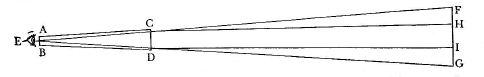
\includegraphics[max width=0.82\textwidth,max height=0.45\textheight,keepaspectratio]{images/figura05.png}\vspace{0.35em}\end{center}
Sit enim, facilioris intelligentiæ gratia, tubus ABCD. Oculus inspicientis esto E. Radii, dum nulla in tubo adessent Perspicilla, ad obiectum FG secundum lineas rectas ECF, EDG ferrentur; sed, appositis Perspicillis, ferantur secundum lineas refractas ECH, EDI: coarctantur enim, et qui prius liberi ad FG obiectum dirigebantur, partem tantummodo HI compræhendent. Accepta deinde ratione distantiæ EH ad lineam HI, per tabulam sinuum reperietur quantitas anguli in oculo ex obiecto HI constituti, quem minuta quædam tantum continere comperiemus. Quod si Specillo CD bracteas, alias maioribus, alias vero minoribus perforatas foraminibus, aptaverimus, modo hanc, modo illam, prout opus fuerit, superimponentes, angulos alios atque alios pluribus paucioribusque minutis subtendentes, pro libito constituemus; quorum ope Stellarum intercapedines, per aliquot minuta adinvicem dissitarum, citra unius aut alterius minuti peccatum, commode dimetiri poterimus. Hæc tamen sic leviter tetigisse, et quasi primoribus libasse labiis, in præsentiarum sit satis; per aliam enim occasionem absolutam huius Organi theoriam in medium proferemus. Nunc observationes a nobis duobus proxime elapsis mensibus habitas recenseamus, ad magnarum profecto contemplationum exordia omnes veræ philosophiæ\textsc{ }cupidos convocantes.

De facie autem Lunæ, quæ ad aspectum nostrum vergit, primo loco dicamus. Quam, facilioris intelligentiæ gratia, in duas partes distinguo, alteram nempe clariorem, obscuriorem alteram: clarior videtur totum hemisphærium ambire atque perfundere, obscurior vero, veluti nubes quædam, faciem ipsam inficit maculosamque reddit. Istæ autem maculæ, subobscuræ et satis amplæ, unicuique sunt obviæ, illasque ævum omne conspexit; quapropter magnas, seu antiquas, eas appellabimus, ad differentiam aliarum macularum amplitudine minorum, at frequentia ita consitarum, ut totam Lunarem superficiem, præsertim vero lucidiorem partem, conspergant; hæ vero a nemine ante nos observatæ fuerunt: ex ipsarum autem sæpius iteratis inspectionibus in eam deducti sumus sententiam, ut certo intelligamus, Lunæ superficiem, non perpolitam, æquabilem, exactissimæque sphæricitatis existere, ut magna philosophorum cohors de ipsa deque reliquis corporibus cælestibus opinata est, sed, contra, inæqualem, asperam, cavitatibus tumoribusque confertam, non secus ac ipsiusmet Telluris facies, quæ montium iugis valliumque profunditatibus hinc inde distinguitur. Apparentiæ vero, ex quibus haec colligere licuit, eiusmodi sunt.

Quarta aut quinta post coniunctionem\textsc{ }die, cum splendidis Luna sese nobis cornibus offert, iam terminus partem obscuram a luminosa dividens non æquabiliter secundum ovalem lineam extenditur, veluti in solido perfecte sphærico accideret; sed inæquabili, aspera et admodum sinuosa linea designatur, veluti apposita figura repræsentat: complures enim veluti excrescentiæ lucidæ ultra lucis tenebrarumque confinia in partem obscuram extenduntur, et, contra, tenebricosæ particulæ intra lumen ingrediuntur. Quinimmo, et magna nigricantium macularum exiguarum copia, omnino a tenebrosa parte separatarum, totam fere plagam iam Solis lumine perfusam undiquaque conspergit, illa saltem excepta parte, quæ magnis et antiquis maculis est affecta. Adnotavimus autem, modo dictas exiguas maculas in hoc semper et omnes, convenire, ut partem habeant nigricantem locum Solis respicientem; ex adverso autem Solis lucidioribus terminis, quasi candentibus iugis coronentur. At consimilem penitus aspectum habemus in Terra circa Solis exortum, dum valles nondum lumine perfusas, montes vero illas ex adverso Solis circundantes iam iam splendore fulgentes intuemur: ac veluti terrestrium cavitatum umbræ, Sole sublimiora petente, imminuuntur, ita et lunares istæ maculæ, crescente parte luminosa, tenebras amittunt.\footnote{\textsuperscript{Vedi figura 1.}}

\begin{center}\vspace{0.6em}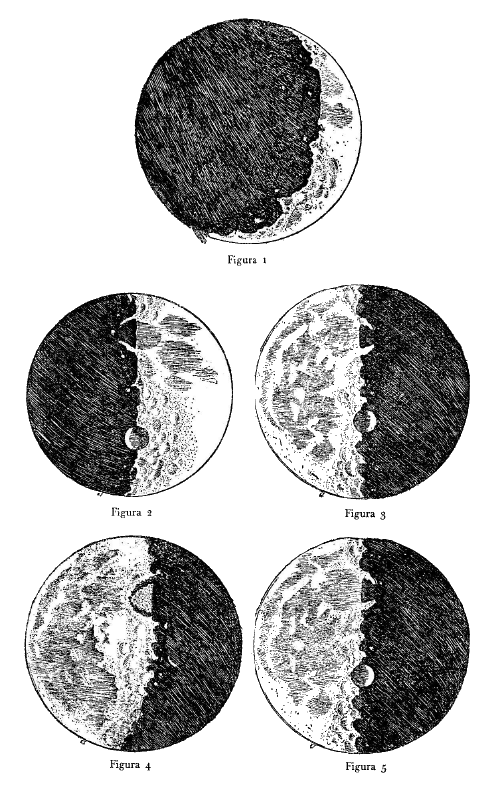
\includegraphics[max width=0.88\textwidth,max height=0.72\textheight,keepaspectratio]{images/figura01.png}\vspace{0.6em}\end{center}

Verum, non modo tenebrarum et luminis confinia in Luna inæqualia ac sinuosa cernuntur; sed, quod maiorem infert admirationem, permultæ apparent lucidæ cuspides intra tenebrosam Lunæ partem, omnino ab illuminata plaga divisæ et avulsæ, ab eaque non per exiguam intercapedinem dissitæ; quæ paulatim, aliqua interiecta mora, magnitudine et lumine augentur, post vero secundam horam aut tertiam reliquæ parti lucidæ et ampliori iam factæ iunguntur; interim tamen aliæ atque aliæ, hinc inde quasi pullulantes, intra tenebrosam partem accenduntur, augentur, ac demum eidem luminosæ superficiei, magis adhuc extensæ, copulantur. Huius exemplum eadem figura nobis exhibet. At nonne in terris ante Solis exortum, umbra adhuc planities occupante, altissimorum cacumina montium solaribus radiis illustrantur? Nonne exiguo interiecto tempore ampliatur lumen, dum mediæ et largiores eorundem montium partes illuminantur; ac tandem, orto iam Sole, planicierum et collium illuminationes iunguntur? Huiusmodi autem eminentiarum et cavitatum discrimina in Luna longe lateque terrestrem asperitatem superare videntur, ut infra demonstrabimus. Interim silentio minime involvam quid animadversione dignum a me observatum, dum Luna ad primam quadraturam properaret, cuius etiam imaginem eadem supra posita delineatio præ se fert: ingens enim sinus tenebrosus in partem luminosam subit, versus inferius cornu locatus; quem quidem sinum cum diutius observassem, totumque obscurum vidissem, tandem post duas fere horas, paulo infra medium cavitatis, vertex quidam luminosus exsurgere cœpit; hic vero paulatim crescens trigonam figuram præ se ferebat, eratque omnino adhuc a luminosa facie revulsus ac separatus; mox circa illum tres aliæ cuspides exiguæ lucere cœperunt; donec, Luna iam occasum versus tendente, trigona illa figura, extensa et amplior iam facta, cum reliqua luminosa parte nectebatur, ac instar ingentis promontorii, a tribus iam commemoratis lucidis verticibus adhuc obsessa, in tenebrosum sinum erumpebat. In extremis quoque cornibus, tam superiori, quam inferiori, splendida quædam puncta, et omnino a reliquo lumine disiuncta, emergebant, veluti in eadem figura depictum cernitur. Eratque magna obscurarum macularum vis in utroque cornu, maxime autem in inferiori: quarum maiores et obscuriores apparent, quæ termino lucis et tenebrarum viciniores sunt; remotiores vero obscuræ minus ac magis dilutæ. Semper tamen, ut supra quoque meminimus, nigricans ipsius maculæ pars irradiationis solaris locum respicit, splendidior vero limbus nigricantem maculam in parte Soli aversa, et Lunæ tenebrosam plagam respiciente, circundat. Hæc lunaris superficies, qua maculis, instar pavonis caudæ cæruleis oculis, distinguitur, vitreis illis vasculis redditur consimilis, quæ adhuc calentia in frigidam immissa, perfractam undosamque superficiem acquirunt, ex quo a vulgo glaciales Gyathi nuncupantur. Verum magnæ eiusdem Lunæ maculæ consimili modo interruptæ atque lacunis et eminentiis confertæ minime cernuntur, sed magis æquabiles et uniformes; solummodo enim clarioribus nonnullis areolis hac illac scatent; adeo ut, si quis veterem Pythagoreorum sententiam exsuscitare velit, Lunam scilicet esse quasi Tellurem alteram, eius pars lucidior terrenam superficiem, obscurior vero aqueam, magis congrue repræsentet: mibi autem dubium fuit nunquam, terrestris globi a longe conspecti atque a radiis solaribus perfusi, terream superficiem clariorem, obscuriorem vero aqueam, sese in conspectum daturam. Depressiores insuper in Luna cernuntur magnæ maculæ, quam clariores plagæ; in illa enim, tam crescente quam decrescente, semper in lucis tenebrarumque confinio prominent hinc inde circa ipsas magnas maculas contermini partis lucidioris, veluti in describendis figuris observavimus: neque depressiores tantummodo sunt dictarum macularum termini, sed æquabiliores, nec rugis aut asperitatibus interrupti. Lucidior vero pars maxime prope maculas eminet; adeo ut, et ante quadraturam primam, et in ipsa ferme secunda, circa maculam quandam, superiorem, borealem nempe, Lunæ plagam occupantem, valde attollantur, tam supra illam quam infra, ingentes quædam eminentiæ, veluti appositæ præ se ferunt delineationes.\footnote{\textsuperscript{Vedi figure 2 e 3.}}~

Hæc eadem macula ante secundam quadraturam nigrioribus quibusdam terminis circumvallata conspicitur; qui, tanquam altissima montium iuga, ex parte Soli aversa obscuriores apparent, qua vero Solem respiciunt lucidiores extant: cuius oppositum in cavitatibus accidit; quarum pars Soli aversa splendens apparet, obscura vero ac umbrosa quæ ex parte Solis sita est. Imminuta deinde luminosa superficie, cum primum tota ferme dicta macula tenebris est obducta, clariora montium dorsa eminenter tenebras scandunt. Hanc duplicem apparentiam sequentes figuræ commonstrant.\footnote{\textsuperscript{Vedi figure 4 e 5.}}

Unum quoque oblivioni minime tradam, quod non nisi aliqua cum admiratione adnotavi: medium quasi Lunæ locum a cavitate quadam occupatum esse reliquis omnibus maiori, ac figura perfectæ rotunditatis; hanc prope quadraturas ambas conspexi, eandemque in secundis supra positis figuris quantum licuit imitatus sum: eundem, quo ad obumbrationem et illuminationem, facit aspectum, ac faceret in terris regio consimilis Bohemiæ, si montibus altissimis, inque peripheriam perfecti circuli dispositis, occluderetur undique; in Luna enim adeo elatis iugis vallatur, ut extrema ora tenebrosæ Lunæ parti contermina, Solis lumine perfusa spectetur, priusquam lucis umbræque terminus ad mediam ipsius figuræ diametrum pertingat. De more autem reliquarum macularum, umbrosa illius pars Solem respicit, luminosa vero versus tenebras Lunæ constituitur; quod tertio libenter observandum admoneo, tanquam firmissimum argumentum asperitatum inæqualitatumque per totam Lunæ clariorem plagam dispersarum: quarum quidem macularum semper nigriores sunt illæ, quæ confinio luminis et tenebrarum conterminæ sunt, remotiores vero tum minores, tum obscuræ minus apparent; ita ut tandem, cum Luna in oppositione totum impleverit orbem, modico admodumque tenui discrimine cavitatum opacitas ab eminentiarum candore discrepet.

Hæc, quæ recensuimus, in clarioribus Lunæ regionibus observantur; verum in magnis maculis talis non conspicitur lacunarum eminentiarumque differentia, qualem necessario constituere cogimur in parte lucidiori, ob mutationem figurarum ex alia atque alia illuminatione radiorum Solis, prout multiplici positu Lunam respicit: at in magnis maculis existunt quidem areolæ nonnullæ subobscuriores, veluti in figuris adnotavimus; attamen istæ eundem semper faciunt aspectum, neque intenditur earum opacitas aut remittitur, sed exiguo admodum discrimine paululum obscuriores modo apparent, modo vero clariores, si magis aut minus obliqui in eas radii solares incidant: iunguntur præterea cum proximis macularum partibus leni quadam copula, confinia miscentes ac confundentes: secus vero in maculis accidit splendidiorem Lunæ superficiem occupantibus; quasi enim abruptæ rupes asperis et angulatis scopulis consitæ, umbrarum luminumque rudibus discriminibus ad lineam disterminantur. Spectantur insuper intra easdem magnas maculas areolæ quædam, aliæ clariores, imo nonnullæ lucidissimae: verum, et harum et obscuriorum, idem semper est aspectus, nulla aut figurarum aut lucis aut opacitatis mutatio; adeo ut compertum indubitatumque sit, apparere illas ob veram partium dissimilaritatem, non autem ob inæqualitates tantum in figuris earundem partium, umbras ex variis Solis illuminationibus diversimode moventibus: quod bene contingit de maculis aliis minoribus clariorem Lunæ partem occupantibus; in dies enim permutantur, augentur, imminuuntur, abolentur, quippe quæ ab umbris tantum eminentiarum ortum ducunt.

Verum magna hic dubitatione complures affici sentio, adeoque gravi difficultate occupari, ut iam explicatam et tot apparentiis confirmatam conclusionem in dubium revocare cogantur. Si enim pars illa lunaris superficiei, quæ splendidius solares radios retorquet, anfractibus, tumoribus scilicet et lacunis innumeris, est repleta, cur in crescenti Luna extrema circumferentia, quæ occasum versus spectat, in decrescenti vero altera semicircumferentia orientalis, ac in plenilunio tota peripheria, non inæquabilis, aspera et sinuosa, verum exacte rotunda et circinata nullisque tumoribus aut cavitatibus corrosa, conspicitur? atque ex eo maxime, quia totus integer limbus ex clariori Lunæ substantia constat, quam tuberosam lacunosamque totam esse diximus; magnarum enim macularum nulla ad extremum usque perimetrum exporrigitur, sed omnes procul ab orbita aggregatæ cernuntur. Huius apparentiæ, ansam tam graviter dubitandi præbentis, duplicem causam, ac proinde duplicem dubitationis solutionem, in medium affero. Primo enim, si tumores et cavitates in corpore lunari secundum unicam tantum circuli peripheriam, hemisphærium nobis conspicuum terminantem, protenderentur, tunc posset quidem, imo deberet, Luna sub specie quasi dentatæ rotæ sese nobis ostendere, tuberoso, nempe, ac sinuoso ambitu terminata: at si non una tantum eminentiarum series, iuxta unicam solummodo circumferentiam dispositarum, sed permulti montium ordines cum suis lacunis et anfractibus circa extremum Lunæ ambitum coordinati fuerint, iique non modo in hemisphærio apparente, sed in averso etiam (prope tamen hemisphæriorum finitorem), tunc oculus a longe prospiciens eminentiarum cavitatumque discrimina depræhendere minime poterit; intercapedines enim montium, in eodem circulo seu in eadem serie dispositorum, obiectu aliarum eminentiarum in aliis atque aliis ordinibus constitutarum occultantur; idque maxime, si oculus aspicientis in eadem recta cum dictarum eminentiarum verticibus fuerit locatus. Sic in terra multorum ac frequentium montium iuga secundum planam superficiem disposita apparent, si prospiciens procul fuerit et in pari altitudine constitutus. Sic æstuosi pelagi sublimes undarum vertices secundum idem planum videntur extensi, quamvis inter fluctus maxima voraginum et lacunarum sit frequentia, adeoque profundarum, ut sublimium navigiorum non modo carinæ, verum etiam puppes, mali ac vela inter illas abscondantur. Quia igitur in ipsa Luna et circa eius perimetrum multiplex est eminentiarum et cavitatum coordinatio, et oculus e longinquo spectans in eodem fere plano cum verticibus illarum locatur; nemini mirum esse debet, quod radio visorio illos abradenti, secundum æquabilem lineam minimeque anfractuosam sese offerant. Huic rationi altera subnecti potest: quod nempe circa lunare corpus est, veluti circa Terram, orbis quidam densioris substantiæ reliquo æthere, qui Solis irradiationem concipere atque reflectere valet, quamvis tanta non sit opacitate præditus, ut visui (præsertim dum illuminatus non fuerit) transitum inhibere valeat. Orbis iste a radiis solaribus illuminatus lunare corpus sub maioris sphæræ speciem reddit repræsentatque; essetque potis aciem nostram terminare, quominus ad Lunæ soliditatem pertingeret, si crassities eius foret profundior: atque profundior quidem est circa Lunæ peripheriam; profundior, inquam, non absolute, sed ad radios nostros, oblique illum secantes, relatus: ac proinde visum nostrum inhibere potest, ac præsertim luminosus existens, Lunæque peripheriam Soli expositam obtegere. Quod clarius in apposita figura intelligitur, in qua lunare corpus ABC ab orbe vaporoso circundatur DEG; oculus vero ex F ad partes intermedias Lunæ, ut ad A, pertingit per vapores DA minus profundos: at versus extremam oram, profundiorum copia vaporum EB aspectum nostrum suo termino præcludit. Signum huius est, quod pars Lunæ lumine perfusa amplioris circumferentiæ apparet, quam reliquum orbis tenebrosi: atque hanc eandem causam quispiam forte rationabilem existimabit, cur maiores Lunæ maculæ nulla ex parte ad extremum usque ambitum protendi conspiciantur, cum tamen opinabile sit nonnullas etiam circa illum reperiri; inconspicuas tamen esse credibile videtur ex eo, quod sub profundiori ac lucidiori vaporum copia abscondantur.
\begin{center}\vspace{0.35em}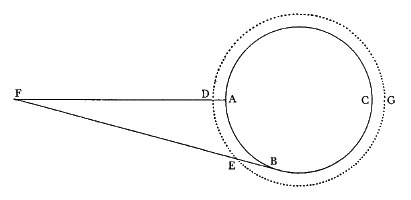
\includegraphics[max width=0.82\textwidth,max height=0.45\textheight,keepaspectratio]{images/figura06.png}\vspace{0.35em}\end{center}


Esse igitur clariorem Lunæ superficiem tumoribus atque lacunis undiquaque conspersam, ex iam explicatis apparitionibus satis apertum esse reor. Superest ut de illorum magnitudinibus dicamus, demonstrantes terrestres asperitates lunaribus esse longe minores; minores, inquam, etiam absolute loquendo, non autem in ratione tantum ad suorum globorum magnitudines: idque sic manifeste declaratur.

Cum sæpius a me observatum sit in aliis atque aliis Lunæ ad Solem constitutionibus, vertices nonnullos intra tenebrosam Lunæ partem, licet a termino lucis satis remotos, lumine perfusos apparere, conferens eorum distantiam ad integram Lunæ diametrum, cognovi, interstitium hoc vigesimam interdum diametri partem superare.

Quo sumpto, intelligatur lunaris globus, cuius maximus circulus CAF, centrum vero E, dimetiens CF, qui ad Terræ diametrum est ut duo ad septem; cumque terrestris diameter, secundum exactiores observationes, milliaria Italica 7000 contineat, erit CF 2000, CE vero 1000; pars autem vigesima totius CF, milliaria 100. Sit modo CF dimetiens circuli maximi, luminosam Lunæ partem ab obscura dividentis (ob maximam enim elongationem Solis a Luna hic circulus a maximo sensibiliter non differt), ac secundum vigesimam illius partem distet A a puncto C, et protrahatur semidiameter EA, qui extensus occurrat cum contingente GCD (quæ radium illuminantem repræsentat) in puncto D. Erit igitur arcus CA, seu recta CD, 100 qualium CE est 1000, et aggregatum quadratorum DC, CE 1.010.000, cui quadratum DE æquale est: tota igitur ED erit plusquam 1004, et AD plusquam 4 qualium CE fuit 1000. Sublimitas igitur AD in Luna, quæ verticem quempiam ad usque Solis radium GCD elatum, et a termino C per distantiam CD remotum, designat, eminentior est milliaribus Italicis 4. Verum in Tellure nulli extant montes, qui vix ad unius milliarii altitudinem perpendicularem accedant; manifestum igitur relinquitur, lunares eminentias terrestribus esse sublimiores.

\begin{center}\vspace{0.35em}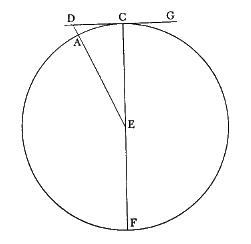
\includegraphics[max width=0.82\textwidth,max height=0.45\textheight,keepaspectratio]{images/figura07.png}\vspace{0.35em}\end{center}
Lubet hoc loco alterius cuiusdam lunaris apparitionis, admiratione dignæ, causam assignare; quæ licet a nobis non recens, sed multis abhinc annis, observata sit, nonnullisque familiaribus amicis et discipulis ostensa, explicata atque per causam declarata, quia tamen eius observatio Perspicilli ope facilior redditur atque evidentior, non incongrue hoc in loco reponendam esse duxi; idque etiam tum maxime, ut cognatio atque similitudo inter Lunam atque Tellurem clarius appareat.

Dum Luna, tum ante tum etiam post coniunctionem, non procul a Sole reperitur, non modo ipsius globus, ex parte qua lucentibus cornibus exornatur, visui nostro spectandum sese offert; verum etiam tenuis quædam sublucens peripheria tenebrosæ partis, Soli nempe aversæ, orbitam delineare, atque ab ipsius ætheris obscuriori campo seiungere, videtur. Verum, si exactiori inspectione rem consideremus, videbimus, non tantum extremum tenebrosæ partis limbum incerta quadam claritate lucentem, sed integram Lunæ faciem, illam nempe quæ Solis fulgorem nondum sentit, lumine quodam, nec exiguo, albicare: apparet tamen primo intuitu subtilis tantummodo circumferentia lucens propter obscuriores Cæli partes sibi conterminas; reliqua vero superficies obscurior e contra videtur ob fulgentium cornuum, aciem nostram obtenebrantium, contactum. Verum si quis talem sibi eligat situm, ut a tecto vel camino aut aliquo alio obice inter visum et Lunam (sed procul ab oculo posito) cornua ipsa lucentia occultentur, pars vero reliqua lunaris globi aspectui nostro exposita relinquatur; tunc luce non exigua hanc quoque Lunæ plagam, licet solari lumine destitutam, splendere depræhendet, idque potissimum, si iam nocturnus horror ob Solis absentiam increverit; in campo enim obscuriori eadem lux clarior apparet. Compertum insuper est, hanc secundam (ut ita dicam) Lunæ claritatem maiorem esse, quo ipsa minus a Sole distiterit: per elongationem enim ab eo remittitur magis magisque, adeo ut post primam quadraturam, et ante secundam, debilis et admodum incerta comperiatur, licet in obscuriori Cælo spectetur; cum tamen in sextili et minori elongatione, quamvis inter crepuscula, mirum in modum fulgeat; fulgeat, inquam, adeo, ut ope exacti Perspicilli magnæ maculæ in ipsa distinguantur. Hic mirabilis fulgor non modicam philosophantibus intulit admirationem; pro cuius causa afferenda alii alia in medium protulerunt. Quidam enim proprium esse ac naturalem ipsiusmet Lunæ splendorem dixerunt; alii, a Venere illi esse impertitum; alii, a stellis omnibus; alii, a Sole, qui radiis suis profundam Lunæ soliditatem permeet. Verum huiuscemodi prolata exiguo labore coarguuntur, ac falsitatis evincuntur. Si enim aut proprium esset aut a Stellis collatum eiusmodi lumen, illud maxime in Eclipsibus retineret ostenderetque, cum in obscurissimo Cælo destituatur; quod tamen adversatur experientiæ: fulgor enim, qui in deliquiis apparet in Luna, longe minor est, subrufus ac quasi æneus; hic vero clarior et candidior. Est insuper ille mutabilis ac loco mobilis; vagatur enim per Lunæ faciem, adeo ut pars illa, quæ peripheriæ circuli umbræ terrestris propinquior est, clarior, reliqua vero obscurior, semper spectetur: ex quo omni procul dubio id accidere intelligimus, ex radiorum Solarium vicinitate tangentium crassiorem quandam regionem, quæ Lunam orbiculariter ambit; ex quo contactu Aurora quædam in vicinas Lunæ plagas effunditur, non secus ac in terris, tum mane, tum vesperi, crepusculinum spargitur lumen: qua de re fusius in libro \textit{De systemate mundi} pertractabimus. Asserere autem a Venere impertitam eiusmodi lucem, puerile adeo est, ut responsione sit indignum. Quis enim adeo inscius erit, ut non intelligat, circa coniunctionem et intra sextilem aspectum partem Lunæ Soli aversam, ut a Venere spectetur, omnino esse impossibile? Esse autem ex Sole, qui suo lumine profundam Lunæ soliditatem penetret atque perfundat, pariter est inopinabile: numquam enim imminueretur, cum semper hemisphærium Lunæ a Sole sit illustratum, tempore lunarium Eclipsium excepto; diminuitur tamen dum Luna ad quadraturam properat, et omnino etiam hebetatur, dum quadraturam superaverit. Cum itaque eiusmodi secundarius fulgor nec Lunæ sit congenitus atque proprius, nec a Stellis ullis nec a Sole mutuatus, cumque iam in Mundi vastitate corpus aliud supersit nullum, nisi sola Tellus, quid, quæso, opinandum? quid proferendum? nunquid a Terra ipsum lunare corpus, aut quidpiam aliud opacum atque tenebrosum lumine perfundi? quid mirum? maxime: æqua grataque permutatione rependit Tellus parem illuminationem ipsi Lunæ, qualem et ipsa a Luna in profundioribus noctis tenebris toto fere tempore recipit. Rem clarius aperiamus. Luna in coniunctionibus, cum medium inter Solem et Terram obtinet locum, solaribus radiis in superiori suo hemisphærio Terræ averso perfunditur; hemisphærium vero inferius, quo Terram aspicit, tenebris est obductum; nullatenus igitur terrestrem superficiem illustrat. Luna, paulatim a Sole digressa, iam iam aliqua ex parte in hemisphærio inferiori ad nos vergente illuminatur, albicantia cornua, subtilia tamen, ad nos convertit, et leviter Terram illustrat: crescit in Luna, iam ad quadraturam accedente, Solaris illuminatio, augetur in terris eius luminis reflexio, extenditur adhuc supra semicirculum splendor in Luna, et nostræ clariores effulgent noctes: tandem integer Lunæ vultus, quo terram aspicit, ab opposito Sole clarissimis fulgoribus irradiatur, enitet longe lateque terrestris superficies lunari splendore perfusa: postmodum decrescens Luna debiliores ad nos radios emittit, debilius illuminatur Terra: Luna ad coniunctionem properat, atra nox Terram occupat. Tali itaque periodo alternis vicibus lunaris fulgor menstruas illuminationes, clariores modo, debiliores alias, nobis largitur: verum æqua lance beneficium a Tellure compensatur. Dum enim Luna sub Sole circa coniunctiones reperitur, superficiem terrestris hemisphærii Soli expositi vividisque radiis illustrati integram respicit, reflexumque ab ipsa lumen concipit: ac proinde ex tali reflexione inferius hemisphærium Lunæ, licet solari lumine destitutum, non modice lucens apparet. Eadem Luna, per quadrantem a Sole remota, dimidium tantum terrestris hemisphærii illuminatum conspicit, scilicet occiduum; altera enim medietas orientalis nocte obtenebratur: ergo, et ipsa Luna splendide minus a Terra illustratur, eiusve proinde lux illa secundaria exilior nobis apparet. Quod si Lunam in oppositione ad Solem constituas, spectabit ipsa hemisphærium intermediæ Telluris omnino tenebrosum obscuraque nocte perfusum: si igitur ecliptica fuerit talis oppositio, nullam prorsus illuminationem recipiet Luna, solari simul ac terrestri irradiatione destituta. In aliis atque aliis ad Terram et ad Solem habitudinibus, maius minusve a terrestri reflexione recipit lumen, prout maiorem aut minorem terrestris hemisphærii illuminati partem spectaverit: is enim inter duos hosce globos servatur tenor, ut quibus temporibus maxime a Luna illustratur Tellus, iisdem minus vice versa a Terra illuminetur Luna, et e contra. Atque hæc pauca de hac re in præsenti loco dicta sufficiant, fusius enim in nostro \textit{Systemate Mundi}; ubi, complurimis et rationibus et experimentis, validissima solaris luminis e Terra reflexio ostenditur illis, qui eam a Stellarum corea arcendam esse iactitant, ex eo potissimum quod a motu et a lumine sit vacua; vagam enim illam ac Lunam splendore superantem, non autem sordium mundanarumque fecum sentinam, esse demonstrationibus et naturalibus quoque rationibus sexcentis confirmabimus.

Diximus hucusque de observationibus circa lunare corpus habitis; nunc de Stellis fixis ea, quæ hactenus a nobis inspecta fuerunt, breviter in medium adferamus. Ac primo illud animadversione dignum est, quod scilicet Stellæ, tam fixæ, quam errabundæ, dum adhibito Perspicillo spectantur, nequaquam magnitudine augeri videntur iuxta proportionem eandem, secundum quam obiecta reliqua, et ipsamet quoque Luna, acquirunt incrementa: verum in Stellis talis auctio longe minor apparet; adeo ut Perspicillum, quod reliqua obiecta secundum centuplam, gratia exempli, rationem multiplicare potens erit, vix secundum quadruplam aut quintuplam Stellas multiplices reddere credas. Ratio autem huius est, quod scilicet Astra, dum libera ac naturali oculorum acie spectantur, non secundum suam simplicem nudamque, ut ita dicam, magnitudinem sese nobis offerunt, sed fulgoribus quibusdam irradiata, micantibusque radiis crinita, idque potissimum cum iam increverit nox; ex quo longe maiores videntur, quam si ascititiis illis crinibus essent exuta: angulus enim visorius, non a primario Stellæ corpusculo, sed a late circumfuso splendore, terminatur. Hoc apertissime intelligas licet ex eo, quod Stellæ in Solis occasu inter prima crepuscula emergentes, tametsi primæ fuerint magnitudinis, exiguæ admodum apparent; et Venus ipsa, si quando circa meridiem se nobis in conspectum dederit, adeo exilis cernitur, ut vix Stellulam magnitudinis ultimæ æquare videatur. Secus in aliis obiectis, et in ipsamet Luna, contingit; quæ, sive in meridiana luce sive inter profundiores tenebras spectetur, eiusdem semper molis apparet. Intonsa igitur in mediis tenebris spectantur Astra, crines tamen illorum diurna lux abradere potest; at non lux ista tantum, sed tenuis quoque nubecula, quæ inter Sidus et oculum aspicientis interponatur: idem quoque præstant nigra velamina ac vitra colorata, quorum obiectu atque interpositione circumfusi fulgores Stellas deserunt. Hoc idem pariter efficit Perspicillum: prius enim adscititios accidentalesque a Stellis fulgores adimit, illarum inde globulos simplices (si tamen figura fuerint globosa) auget; atque adeo secundum minorem multiplicitatem adaucta videntur. Stellula enim quintæ aut sextæ magnitudinis, per Perspicillum visa, tamquam magnitudinis primæ repræsentatur.

Adnotatione quoque dignum videtur esse discrimen inter Planetarum atque fixarum Stellarum aspectus. Planetæ enim globulos suos exacte rotundos ac circinatos obiiciunt, ac, veluti Lunulæ quædam undique lumine perfusæ, orbiculares apparent: fixæ vero Stellæ peripheria circulari nequaquam terminatæ conspiciuntur, sed veluti fulgores quidam radios circumcirca vibrantes atque admodum scintillantes; consimili tandem figura præditæ apparent cum Perspicillo, ac dum naturali intuitu, spectantur, sed adeo maiores ut Stellula quintæ aut sextæ magnitudinis Canem, maximam nempe fixarum omnium, æquare videatur. Verum, infra Stellas magnitudinis sextæ, adeo numerosum gregem aliarum, naturalem intuitum fugientium, per Perspicillum intueberis, ut vix credibile sit: plures enim, quam sex aliæ magnitudinum differentiæ, videas licet; quarum maiores, quas magnitudinis septimæ, seu primæ invisibilium, appellare possumus, Perspicilli beneficio maiores et clariores apparent, quam magnitudinis secundæ Sidera, acie naturali visa. Ut autem de inopinabili fere illarum frequentia unam alteramve attestationem videas, Asterismos duos subscribere placuit, ut ab eorum exemplo de cæteris iudicium feras. In primo integram Orionis Constellationem pingere decreveram; verum ab ingenti Stellarum copia, temporis vero inopia, obrutus, aggressionem hanc in aliam occasionem distuli; adstant enim, et circa veteres, intra unius aut alterius gradus limites, disseminantur, plures quingentis: quapropter tribus quæ in Cingulo, et senis quæ in Ense iampridem adnotatæ fuerunt, alias adiacentes octuaginta recens visas apposuimus; earumque interstitia, quo exactius licuit, servavimus: notas, seu veteres, distinctionis gratia, maiores pinximus, ac duplici linea contornavimus; alias inconspicuas, minores, ac unis lineis notavimus; magnitudinum quoque discrimina, quo magis licuit, servavimus.

In altero exemplo sex Stellas Tauri, PLEIADAS dictas, depinximus (dico autem sex, quandoquidem septima fere nunquam apparet) intra angustissimos in Cælo cancellos obclusas, quibus aliæ, plures quam quadraginta, invisibiles adiacent; quarum nulla ab aliqua ex prædictis sex vix ultra semigradum elongatur: harum nos tantum triginta sex adnotavimus; earumque interstitia, magnitudines, necnon veterum novarumque discrimina, veluti in Orione, servavimus.


\begin{center}\vspace{0.6em}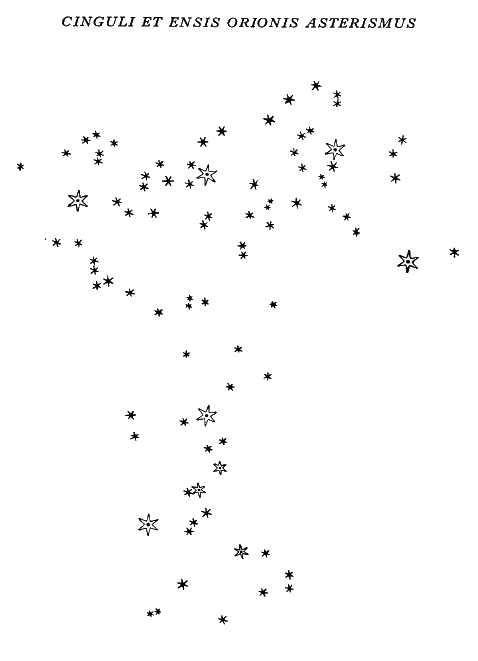
\includegraphics[max width=0.88\textwidth,max height=0.72\textheight,keepaspectratio]{images/figura02.png}\vspace{0.6em}\end{center}


Quod tertio loco a nobis fuit observatum, est ipsiusmet LACTEI Circuli essentia, seu materies, quam Perspicilli beneficio adeo ad sensum licet intueri, ut et altercationes omnes, quæ per tot sæcula philosophos excruciarunt, ab oculata certitudine dirimantur, nosque a verbosis disputationibus liberemur. Est enim GALAXIA nihil aliud, quam innumerarum Stellarum coacervatim consitarum congeries: in quamcumque enim regionem illius Perspicillum dirigas, statim Stellarum ingens frequentia sese in conspectum profert, quarum complures satis magnæ ac valde conspicuæ videntur; sed exiguarum multitudo prorsus inexplorabilis est.

At cum non tantum in GALAXIA lacteus ille candor, veluti albicantis nubis, spectetur, sed complures consimilis coloris areolæ sparsim per æthera subfulgeant, si in illarum quamlibet Specillum convertas, Stellarum constipatarum cœtum offendes. Amplius (quod magis miraberis), Stellæ ab Astronomis singulis in hanc usque diem NEBULOSÆ appellatæ, Stellularum mirum in modum consitarum greges sunt; ex quarum radiorum commixtione, dum unaquæque ob exilitatem, seu maximam a nobis remotionem, oculorum aciem fugit, candor ille consurgit, qui densior pars Cæli, Stellarum aut Solis radios retorquere valens, hucusque creditus est. Nos ex illis nonnullas observavimus, et duarum Asterismos subnectere voluimus.

In primo habes NEBULOSAM, Capitis Orionis appellatam, in qua Stellas vigintiunas numeravimus.

Secundus NEBULOSAM PRÆSEPE nuncupatam continet; quæ non una tantum Stella est, sed congeries Stellularum plurium quam quadraginta: nos, præter Asellos, trigintasex notavimus, in hunc, qui sequitur, ordinem dispositas.


\begin{center}\vspace{0.6em}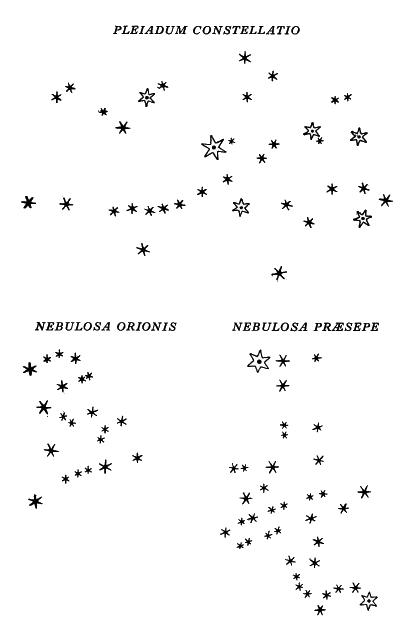
\includegraphics[max width=0.88\textwidth,max height=0.72\textheight,keepaspectratio]{images/figura03.png}\vspace{0.6em}\end{center}


De Luna, de inerrantibus Stellis ac de Galaxia, quæ hactenus observata sunt, breviter enarravimus. Superest ut, quod maximum in præsenti negotio existimandum videtur, quatuor PLANETAS a primo mundi exordio ad nostra usque tempora nunquam conspectos, occasionem reperiendi atque observandi, necnon ipsorum loca, atque per duos proxime menses observationes circa eorundem lationes ac mutationes habitas, aperiamus ac promulgemus; Astronomos omnes convocantes, ut ad illorum periodos inquirendas atque definiendas se conferant, quod nobis in hanc usque diem, ob temporis angustiam, assequi minime licuit. Illos tamen iterum monitos facimus, ne ad talem inspectionem incassum accedant, Perspicillo exactissimo opus esse, et quale in principio sermonis huius descripsimus.

Die itaque septima Ianuarii, instantis anni millesimi sexcentesimi decimi, hora sequentis noctis prima, cum cælestia sidera per Perspicillum spectarem, Iuppiter sese obviam fecit; cumque admodum excellens mihi parassem instrumentum (quod antea ob alterius organi debilitatem minime contigerat), tres illi adstare Stellulas, exiguas quidem, veruntamen clarissimas, cognovi; quæ, licet e numero inerrantium a me crederentur, nonnullam tamen intulerunt admirationem, eo quod secundum exactam lineam rectam atque Eclipticæ parallelam dispositæ videbantur, ac cæteris magnitudine paribus splendidiores. Eratque illarum inter se et ad Iovem talis constitutio:

\begin{center}\vspace{0.35em}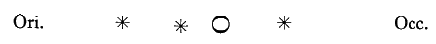
\includegraphics[max width=0.82\textwidth,max height=0.45\textheight,keepaspectratio]{images/figura08.png}\vspace{0.35em}\end{center}
ex parte scilicet orientali duæ aderant Stellæ, una vero occasum versus. Orientalior atque occidentalis, reliqua paulo maiores apparebant: de distantia inter ipsas et Iovem minime sollicitus fui; fixæ enim, uti diximus primo, creditæ fuerunt. Cum autem die octava, nescio quo fato ductus, ad inspectionem eandem reversus essem, longe aliam constitutionem reperi: erant enim tres Stellulæ occidentales omnes, a Iove atque inter se, quam superiori nocte, viciniores, paribusque interstitiis mutuo disseparatæ, veluti apposita præsefert delineatio.

\begin{center}\vspace{0.35em}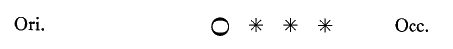
\includegraphics[max width=0.82\textwidth,max height=0.45\textheight,keepaspectratio]{images/figura09.png}\vspace{0.35em}\end{center}
Hic, licet ad mutuam Stellarum appropinquationem minime cogitationem appulissem, hæsitare tamen cœpi, quonam pacto Iuppiter ab omnibus prædictis fixis posset orientalior reperiri, cum a binis ex illis pridie occidentalis fuisset: ac proinde veritus sum ne forte secus a computo astronomico directus foret, ac propterea motu proprio Stellas illas antevertisset. Quapropter maximo cum desiderio sequentem expectavi noctem; verum a spe frustratus fui, nubibus enim undiquaque obductum fuit cælum.

At die decima apparuerunt Stellæ in eiusmodi ad Iovem positu:

\begin{center}\vspace{0.35em}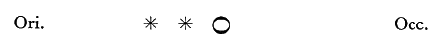
\includegraphics[max width=0.82\textwidth,max height=0.45\textheight,keepaspectratio]{images/figura10.png}\vspace{0.35em}\end{center}
duæ enim tantum, et orientales ambæ, aderant; tertia, ut opinatus fui, sub Iove latitante. Erant pariter, veluti antea, in eadem recta cum Iove, ac iuxta Zodiaci longitudinem adamussim locatæ. Hæc cum vidissem, cumque mutationes consimiles in Iove nulla ratione reponi posse intelligerem, atque insuper spectatas Stellas semper easdem fuisse cognoscerem (nullæ enim aliæ, aut præcedentes, aut consequentes, intra magnum intervallum iuxta longitudinem Zodiaci aderant), iam ambiguitatem in admirationem permutans, apparentem commutationem, non in Iove, sed in Stellis adnotatis repositam esse comperi; ac proinde oculate et scrupulose magis deinceps observandum fore sum ratus.

Die itaque undecima eiuscemodi constitutionem vidi:

\begin{center}\vspace{0.35em}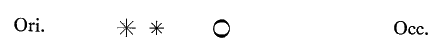
\includegraphics[max width=0.82\textwidth,max height=0.45\textheight,keepaspectratio]{images/figura11.png}\vspace{0.35em}\end{center}
Stellas scilicet tantum duas orientales; quarum media triplo distabat a Iove, quam ab orientaliori, eratque orientalior duplo fere maior reliqua, cum tamen antecedenti nocte æquales ferme apparuissent. Statutum ideo omnique procul dubio a me decretum fuit, tres in cælis adesse Stellas vagantes circa Iovem, instar Veneris atque Mercurii circa Solem; quod tandem luce meridiana clarius in aliis postmodum compluribus inspectionibus observatum est: ac non tantum tres, verum quatuor esse vaga Sidera circa Iovem suas circumvolutiones obeuntia; quorum permutationes, exactius consequenter observatas, subsequens narratio ministrabit: interstitia quoque inter ipsa per Perspicillum, superius explicata ratione, dimetitus sum: horas insuper observationum, præsertim cum plures in eadem nocte habitæ fuerunt, apposui; adeo enim celeres horum Planetarum extant revolutiones, ut horarias quoque differentias plerunque liceat accipere.

Die igitur duodecima, hora sequentis noctis prima, hac ratione disposita Sidera vidi:

\begin{center}\vspace{0.35em}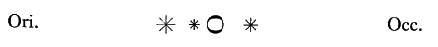
\includegraphics[max width=0.82\textwidth,max height=0.45\textheight,keepaspectratio]{images/figura12.png}\vspace{0.35em}\end{center}
erat orientalior Stella occidentaliori maior, ambæ tamen valde conspicuæ ac splendidæ: utraque distabat a Iove scrupulis primis duobus: tertia quoque Stellula apparere cœpit hora tertia, prius minime conspecta, quæ ex parte orientali Iovem fere tangebat, eratque admodum exigua. Omnes fuerunt in eadem recta et secundum Eclipticæ longitudinem coordinatæ.

Die decimatertia primum a me quatuor conspectæ fuerunt Stellulæ in hac ad Iovem constitutione:

\begin{center}\vspace{0.35em}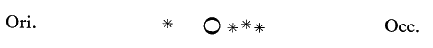
\includegraphics[max width=0.82\textwidth,max height=0.45\textheight,keepaspectratio]{images/figura13.png}\vspace{0.35em}\end{center}
erant tres occidentales et una orientalis: lineam proxime rectam constituebant; media enim occidentalium paululum a recta septentrionem versus deflectebat. Aberat orientalior a Iove minuta duo: reliquarum et Iovis intercapedines erant singulae unius tantum minuti. Stellæ omnes eandem præ se ferebant magnitudinem, ac, licet exiguam, lucidissimæ tamen erant ac fixis eiusdem magnitudinis longe splendidiores.

Die decimaquarta nubilosa fuit tempestas.

Die decimaquinta, hora noctis tertia, in proxime depicta fuerunt habitudine quatuor Stellæ ad Iovem:

\begin{center}\vspace{0.35em}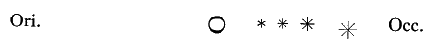
\includegraphics[max width=0.82\textwidth,max height=0.45\textheight,keepaspectratio]{images/figura14.png}\vspace{0.35em}\end{center}
occidentales omnes ac in eadem proxime recta linea dispositæ; quæ enim tertia a Iove numerabatur paululum in boream attollebatur: propinquior Iovi erat omnium minima, reliquæ consequenter maiores apparebant: intervalla inter Iovem et tria consequentia Sidera erant æqualia omnia ac duorum minutorum; at occidentalius aberat a sibi propinquo minutis quatuor. Erant lucida valde, et nihil scintillantia, qualia semper, tum ante, tum post, apparuerunt. Verum hora septima tres solummodo aderant Stellæ, in huiuscemodi cum Iove aspectu:

\begin{center}\vspace{0.35em}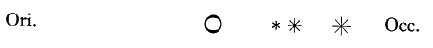
\includegraphics[max width=0.82\textwidth,max height=0.45\textheight,keepaspectratio]{images/figura15.png}\vspace{0.35em}\end{center}
erant nempe in eadem recta ad unguem: vicinior Iovi erat admodum exigua, et ab illo semota per minuta prima tria; ab hac secunda distabat min. uno; tertia vero a secunda min. pr. 4, sec. 30. Post vero aliam horam duæ Stellulæ mediæ adhuc viciniores erant: aberant enim min. sc. vix 30 tantum.

Die decimasexta, hora prima noctis, tres vidimus Stellas iuxta hunc ordinem dispositas:

\begin{center}\vspace{0.35em}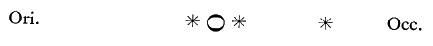
\includegraphics[max width=0.82\textwidth,max height=0.45\textheight,keepaspectratio]{images/figura16.png}\vspace{0.35em}\end{center}
duae Iovem intercipiebant, ab eo per min. 0, sec. 40 hinc inde remotæ; tertia vero occidentalis a Iove distabat min. 8. Iovi proximæ non maiores, sed lucidiores apparebant remotiori.

Die decimaseptima, hora ab occasu 0, min. 30, huiusmodi fuit configuratio:

\begin{center}\vspace{0.35em}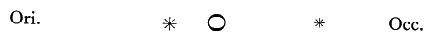
\includegraphics[max width=0.82\textwidth,max height=0.45\textheight,keepaspectratio]{images/figura17.png}\vspace{0.35em}\end{center}
Stella una tantum orientalis a Iove distabat min. 3; occidentalis pariter una, a Iove distans min. 11. Orientalis duplo maior apparebat occidentali; nec plures aderant quam istæ duæ. Verum post horas quatuor, hora nempe proxime quinta, tertia ex parte orientali emergere cœpit, quæ antea, ut opinor, cum priori iuncta erat; fuitque talis positio:

\begin{center}\vspace{0.35em}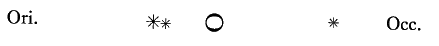
\includegraphics[max width=0.82\textwidth,max height=0.45\textheight,keepaspectratio]{images/figura18.png}\vspace{0.35em}\end{center}
Media Stella, orientali quam proxima, min. tantum sec. 20 elongabatur ab illa, et a linea recta, per extremas et Iovem producta, paululum versus austrum declinabat.

Die decima octava, hora 0, min. 20 ab occasu, talis fuit aspectus:

\begin{center}\vspace{0.35em}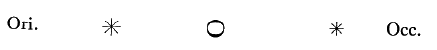
\includegraphics[max width=0.82\textwidth,max height=0.45\textheight,keepaspectratio]{images/figura19.png}\vspace{0.35em}\end{center}
erat Stella orientalis maior occidentali, et a Iove distans min. pr. 8: occidentalis vero a Iove aberat min. 10.

Die decimanona, hora noctis secunda, talis fuit Stellarum coordinatio:

\begin{center}\vspace{0.35em}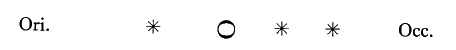
\includegraphics[max width=0.82\textwidth,max height=0.45\textheight,keepaspectratio]{images/figura20.png}\vspace{0.35em}\end{center}
erant nempe secundum rectam lineam ad unguem tres cum Iove Stellæ: orientalis una, a Iove distans min. pr. 6: inter Iovem et primam sequentem occidentalem mediabat min. 5 interstitium: hæc autem ab occidentaliori aberat min. 4. Anceps eram tunc, nunquid inter orientalem Stellam et Iovem Stellula mediaret, verum Iovi quamproxima, adeo ut illum fere tangeret. At, hora quinta, hanc manifeste vidi medium iam inter Iovem et orientalem Stellam locum exquisite occupantem, ita ut talis fuerit configuratio:

\begin{center}\vspace{0.35em}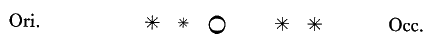
\includegraphics[max width=0.82\textwidth,max height=0.45\textheight,keepaspectratio]{images/figura21.png}\vspace{0.35em}\end{center}
Stella insuper novissime conspecta admodum exigua fuit; veruntamen, hora sexta, reliquis magnitudine fere fuit æqualis.

Die vigesima, hora 1, min. 15, constitutio consimilis visa est:

\begin{center}\vspace{0.35em}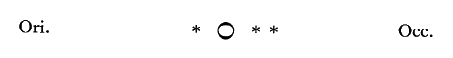
\includegraphics[max width=0.82\textwidth,max height=0.45\textheight,keepaspectratio]{images/figura22.png}\vspace{0.35em}\end{center}
aderant tres Stellulæ adeo exiguæ, ut vix percipi possent: a Iove, et inter se non magis distabant minuto uno: incertus eram, nunquid ex occidente duæ, an tres, adessent Stellulæ. Circa horam sextam hoc pacto erant dispositæ:

\begin{center}\vspace{0.35em}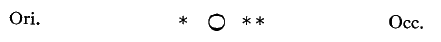
\includegraphics[max width=0.82\textwidth,max height=0.45\textheight,keepaspectratio]{images/figura23.png}\vspace{0.35em}\end{center}
orientalis enim a Iove duplo magis aberat quam antea, nempe min. 2; media occidentalis a Iove distabat min. 0, sec. 40, ab occidentaliori vero min. 0, sec. 20. Tandem, hora septima, tres ex occidente visæ fuerunt Stellulæ:

\begin{center}\vspace{0.35em}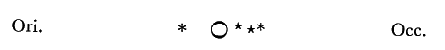
\includegraphics[max width=0.82\textwidth,max height=0.45\textheight,keepaspectratio]{images/figura24.png}\vspace{0.35em}\end{center}
Iovi proxima aberat ab eo min. 0, sec. 20; inter hanc et occidentaliorem intervallum erat minutorum secundorum 40: inter has vero alia spectabatur paululum ad meridiem deflectens, ab occidentaliori non pluribus decem secundis remota.

Die vigesimaprima, hora 0, min. 30, aderant ex oriente Stellulæ tres, æqualiter inter se et a Iove distantes:

\begin{center}\vspace{0.35em}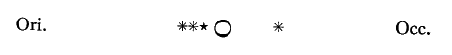
\includegraphics[max width=0.82\textwidth,max height=0.45\textheight,keepaspectratio]{images/figura25.png}\vspace{0.35em}\end{center}
interstitia vero, secundum existimationem, 50 secundorum minutorum fuere. Aderat quoque Stella ex occidente, a Iove distans min. pr. 4. Orientalis Iovi proxima erat omnium minima; reliquæ vero aliquanto maiores, atque inter se proxime æquales.

Die vigesima secunda, hora 2, consimilis fuit Stellarum dispositio:

\begin{center}\vspace{0.35em}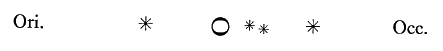
\includegraphics[max width=0.82\textwidth,max height=0.45\textheight,keepaspectratio]{images/figura26.png}\vspace{0.35em}\end{center}
a Stella orientali ad Iovem minutorum primorum 5 fuit intervallum, a Iove ad occidentaliorem pr. 7. Duæ vero occidentales intermediæ distabant ad invicem min. 0, sec. 40; propinquior vero Iovi aberat ab illo m. p. 1. Ipsæ mediæ Stellulæ minores erant extremis: fuerunt vero secundum eandem rectam lineam iuxta Zodiaci longitudinem extensæ, nisi quod trium occidentalium media paululum in austrum deflectebat. Sed, hora noctis sexta, in hac constitutione visæ sunt:

\begin{center}\vspace{0.35em}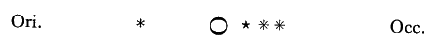
\includegraphics[max width=0.82\textwidth,max height=0.45\textheight,keepaspectratio]{images/figura27.png}\vspace{0.35em}\end{center}
orientalis admodum exigua erat, distans a Iove, ut antea, min. pr. 5. Tres vero occidentales, et a Iove et ad invicem, æqualiter dirimebantur, erantque intercapedines singulæ min. 1, sec. 20 proxime: et Stella Iovi vicinior, reliquis duabus sequentibus minor apparebat: omnesque in eadem recta exquisite dispositæ videbantur.

Die vigesima tertia, hora 0, min. 40 ab occasu, in hunc ferme modum Stellarum constitutio se habuit:

\begin{center}\vspace{0.35em}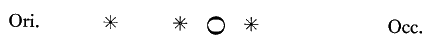
\includegraphics[max width=0.82\textwidth,max height=0.45\textheight,keepaspectratio]{images/figura28.png}\vspace{0.35em}\end{center}
erant tres Stellæ cum Iove in recta linea secundum Zodiaci longitudinem, veluti semper fuerunt: orientales erant duæ, una vero occidentalis. Orientalior aberat a sequenti min. pr. 7, hæc vero a Iove min. 2, sec. 40, Iuppiter ab occidentali min. 3, sec. 20: erantque omnes magnitudine fere æquales. Sed, hora quinta, duæ Stellæ, quæ prius Iovi erant proximæ, amplius non cernebantur, sub Iove, ut arbitror, latitantes; fuitque talis aspectus:

\begin{center}\vspace{0.35em}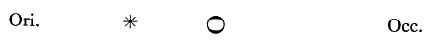
\includegraphics[max width=0.82\textwidth,max height=0.45\textheight,keepaspectratio]{images/figura29.png}\vspace{0.35em}\end{center}
Die vigesimaquarta, tres Stellæ, orientales omnes, visæ sunt, ac fere in eadem cum Iove recta linea:

\begin{center}\vspace{0.35em}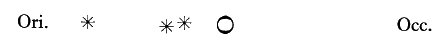
\includegraphics[max width=0.82\textwidth,max height=0.45\textheight,keepaspectratio]{images/figura30.png}\vspace{0.35em}\end{center}
media enim modice in austrum deflectebat. Iovi propinquior distabat ab eo min. 2, sequens ab hac min. 0, sec. 30, ab hac vero aberat orientalior min. 9: erantque omnes admodum spiendidæ. Hora vero sexta, duæ solummodo sese offerebant Stellæ in hoc positu:

\begin{center}\vspace{0.35em}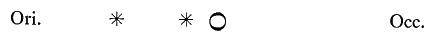
\includegraphics[max width=0.82\textwidth,max height=0.45\textheight,keepaspectratio]{images/figura31.png}\vspace{0.35em}\end{center}
nempe cum Iove in eadem recta linea ad ungem, a quo elongabatur propinquior min. p. 3, altera vero ab hac min. p. 8: in unam, ni fallor, coierant duæ mediæ prius observatæ Stellulæ.

Die vigesimaquinta, hora 1, min. 40, ita se habebat constitutio:

\begin{center}\vspace{0.35em}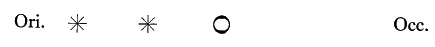
\includegraphics[max width=0.82\textwidth,max height=0.45\textheight,keepaspectratio]{images/figura32.png}\vspace{0.35em}\end{center}
aderant enim duæ tantum Stellæ ex orientali plaga, eæque satis magnæ: orientalior a media distabat min. 5, media vero a Iove min. 6.

Die vigesima sexta, hora 0, min. 40, Stellarum coordinatio eiusmodi fuit:

\begin{center}\vspace{0.35em}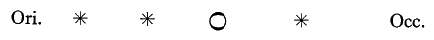
\includegraphics[max width=0.82\textwidth,max height=0.45\textheight,keepaspectratio]{images/figura33.png}\vspace{0.35em}\end{center}
spectabantur enim Stellæ tres, quarum duæ orientales, tertia occidentalis a Iove: hæc ab eo min. 5 aberat, media vero orientalis ab eodem distabat min. 5, sec. 20; orientalior vero a media min. 6: in eadem recta constitutæ, et eiusdem magnitudinis erant. Hora deinde quinta, constitutio fere eadem fuit; in hoc tantum discrepans, quod prope Iovem quarta Stellula ex oriente emergebat, cæteris minor, a Iove tunc remota min. 30, sed paululum a recta linea versus Boream attollebatur, ut apposita figura demonstrat:

\begin{center}\vspace{0.35em}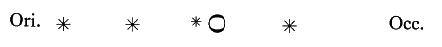
\includegraphics[max width=0.82\textwidth,max height=0.45\textheight,keepaspectratio]{images/figura34.png}\vspace{0.35em}\end{center}
Die vigesima septima, hora 1 ab occasu, unica tantum Stellula conspiciebatur, eaque orientalis, secundum hanc constitutionem:

\begin{center}\vspace{0.35em}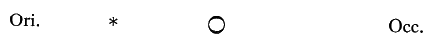
\includegraphics[max width=0.82\textwidth,max height=0.45\textheight,keepaspectratio]{images/figura35.png}\vspace{0.35em}\end{center}
eratque admodum exigua, et a Iove remota min. 7.

Die vigesima octava et vigesima nona, ob nubium interpositionem nihil observare licuit.

Die trigesima, hora prima noctis, tali pacto constituta spectabantur Sidera:

\begin{center}\vspace{0.35em}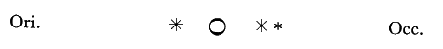
\includegraphics[max width=0.82\textwidth,max height=0.45\textheight,keepaspectratio]{images/figura36.png}\vspace{0.35em}\end{center}
unum aderat orientale, a Iove distans min. 2, sec. 30, duo vero ex occidente, quorum Iovi propinquius aberat ab eo min. 3, reliquum ab hoc min. 1: extremorum et Iovis positus in eadem recta linea fuit, at media Stella paululum in Boream attollebatur: occidentalior fuit reliquis minor.

Die ultima, hora secunda, visæ sunt orientales Stellæie duæ, una vero occidua:

\begin{center}\vspace{0.35em}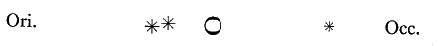
\includegraphics[max width=0.82\textwidth,max height=0.45\textheight,keepaspectratio]{images/figura37.png}\vspace{0.35em}\end{center}
Orientalium media a Iove aberat min. 2, sec. 20; orientalior vero ab ipsa media min. 0, sec. 30; occidentalis distabat a Iove min. 10: erant in eadem recta linea proxime, orientalis tantum Iovi vicinior modicum quiddam in Septentrionem elevabatur. Hora vero quarta,

\begin{center}\vspace{0.35em}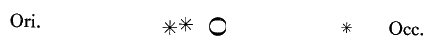
\includegraphics[max width=0.82\textwidth,max height=0.45\textheight,keepaspectratio]{images/figura38.png}\vspace{0.35em}\end{center}
duæ orientales viciniores ad invicem adhuc erant; aberant enim solummodo min. sec. 20. Apparuit in hisce observationibus occidentalis Stella satis exigua.

Die Februarii prima, hora noctis secunda, consimilis fuit constitutio:

\begin{center}\vspace{0.35em}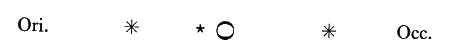
\includegraphics[max width=0.82\textwidth,max height=0.45\textheight,keepaspectratio]{images/figura39.png}\vspace{0.35em}\end{center}
Distabat orientalior Stella a Iove min. 6, occidentalis vero 8; ex parte orientali Stella quædam, admodum exigua, a Iove distabat minutis secundis 20: rectam ad unguem designabant lineam.

Die secunda, iuxta hunc ordinem visæ sunt Stellæ:

\begin{center}\vspace{0.35em}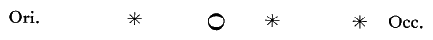
\includegraphics[max width=0.82\textwidth,max height=0.45\textheight,keepaspectratio]{images/figura40.png}\vspace{0.35em}\end{center}
Una tantum orientalis a Iove distabat min. 6; Iuppiter ab occidentali viciniori aberat min. 4; inter hanc et occidentaliorem min. 8 fuit intercapedo: erant in eadem recta ad unguem, et eiusdem fere magnitudinis. Sed, hora septima, quatuor aderant Stellæ:

\begin{center}\vspace{0.35em}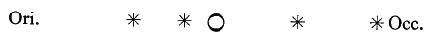
\includegraphics[max width=0.82\textwidth,max height=0.45\textheight,keepaspectratio]{images/figura41.png}\vspace{0.35em}\end{center}
inter quas Iuppiter mediam occupabat sedem. Harum Stellarum orientalior distabat a sequenti min. 4, hæc a Iove min. 1, sec. 40: Iuppiter ab occidentali sibi viciniori aberat min. 6, hæc vero ab occidentaliori min. 8: erantque pariter omnes in eadem recta linea, secundum Zodiaci longitudinem extensa.

Die tertia, hora septima, in hac serie dispositæ fuerunt Stellæ:

\begin{center}\vspace{0.35em}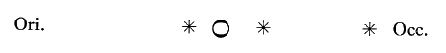
\includegraphics[max width=0.82\textwidth,max height=0.45\textheight,keepaspectratio]{images/figura42.png}\vspace{0.35em}\end{center}
orientalis a Iove distabat min. 1, sec. 30, occidentalis proxima min. 2: ab hac vero elongabatur occidentalior altera min. 10: erant præcise in eadem recta, et magnitudinis æqualis.

Die quarta, hora secunda, circa Iovem quatuor stabant Stellæ, orientales duæ, ac duæ occidentales, in eadem ad unguem recta linea dispositæ, ut in proxima figura:

\begin{center}\vspace{0.35em}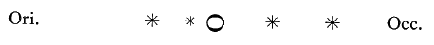
\includegraphics[max width=0.82\textwidth,max height=0.45\textheight,keepaspectratio]{images/figura43.png}\vspace{0.35em}\end{center}
Orientalior distabat a sequenti min. 3, hæc vero a Iove aberat min. 0, sec. 40, Iuppiter a proxima occidentali min. 4, hæc ab occidentaliori min. 6. Magnitudine erant fere æquales; proximior Iovi reliquis paulo minor apparebat. Hora autem septima, orientales Stellæ distabant tantum min. 0, sec. 30.

\begin{center}\vspace{0.35em}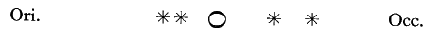
\includegraphics[max width=0.82\textwidth,max height=0.45\textheight,keepaspectratio]{images/figura44.png}\vspace{0.35em}\end{center}
Iuppiter ab orientali viciniori aberat min. 2, ab occidentali vero sequente min. 4, hæc vero ab occidentaliori distabat min. 3: erantque æquales omnes, et in eadem recta secundum Eclipticam extensa.

Die quinta, Cælum fuit nubilosum.

Die sexta, duæ solummodo apparuerunt Stellæ, medium Iovem intercipientes, ut in figura apposita spectatur:

\begin{center}\vspace{0.35em}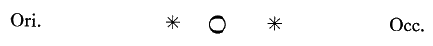
\includegraphics[max width=0.82\textwidth,max height=0.45\textheight,keepaspectratio]{images/figura45.png}\vspace{0.35em}\end{center}
orientalis a Iove distabat min. 2, occidentalis vero min. 3: erant in eadem recta cum Iove, et magnitudine pares.

Die septima, duæ adstabant Stellæ, a Iove orientales ambæ, in hunc dispositæ modum:

\begin{center}\vspace{0.35em}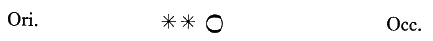
\includegraphics[max width=0.82\textwidth,max height=0.45\textheight,keepaspectratio]{images/figura46.png}\vspace{0.35em}\end{center}
intercapedines inter ipsas et Iovem erant æquales, unius nempe minuti primi; ac per ipsas et centrum Iovis recta linea incedebat.

Die octava, hora prima, aderant tres Stellæ orientales omnes, ut in descriptione:

\begin{center}\vspace{0.35em}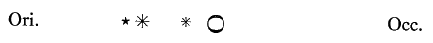
\includegraphics[max width=0.82\textwidth,max height=0.45\textheight,keepaspectratio]{images/figura47.png}\vspace{0.35em}\end{center}
Iovi proxima, exigua satis, distabat ab eo min. 1, sec. 20; media vero ab hac min. 4, eratque satis magna; orientalior, admodum exigua, ab hac distabat min. 0, sec. 20. Anceps eram, nunquid Iovi proxima una tantum, an duæ forent Stellulæ; videbatur enim interdum huic alia adesse versus ortum, mirum in modum exigua, et ab illa seiuncta per min. 0, sec. 10 tantum: fuerunt omnes in eadem recta linea secundum Zodiaci ductum extensæ. Hora vero tertia, Stella Iovi proxima illum fere tangebat; distabat enim ab eo min. 0, sec. 10 tantum: reliquæ vero a Iove remotiores factæ fuerunt; aberat enim media a Iove min. 6. Tandem, hora quarta, quæ prius Iovi proxima erat, cum eo iuncta, non cernebatur amplius.

Die nona, hora 0, m. 30, adstabant Iovi Stellæ duæ orientales, et una occidentalis, in tali dispositione:

\begin{center}\vspace{0.35em}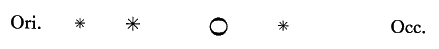
\includegraphics[max width=0.82\textwidth,max height=0.45\textheight,keepaspectratio]{images/figura48.png}\vspace{0.35em}\end{center}
Orientalior, quæ satis exigua erat, a sequenti distabat min. 4; media, maior, a Iove aberat min. 7; Iuppiter ab occidentali, quæ parva erat, distabat min. 4.

Die decima, hora prima, min. 30, Stellulæ binæ, admodum exiguæ, orientales ambæ, in tali dispositione visæ sunt:

\begin{center}\vspace{0.35em}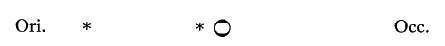
\includegraphics[max width=0.82\textwidth,max height=0.45\textheight,keepaspectratio]{images/figura49.png}\vspace{0.35em}\end{center}
remotior distabat a Iove min. 10, vicinior vero min. 0, sec. 20; erantque in eadem recta. Hora autem quarta, Stella Iovi proxima amplius non apparebat: altera quoque adeo imminuta videbatur, ut vix cerni posset, licet aër præclarus esset; et a Iove remotior, quam antea, erat; distabat siquidem min. 12.

Die undecima, hora prima, aderant ab oriente Stellæ duæ, et una ab occasu. Distabat occidentalis a Iove min. 4; orientalis vicinior

\begin{center}\vspace{0.35em}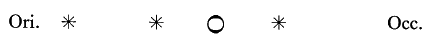
\includegraphics[max width=0.82\textwidth,max height=0.45\textheight,keepaspectratio]{images/figura50.png}\vspace{0.35em}\end{center}
aberat pariter a Iove min. 4; orientalior vero ab hac distabat min. 8: erant satis perspicuæ, et in eadem recta. Sed hora tertia, Stella quarta, Iovi proxima, ab oriente visa est, reliquis minor, a Iove dissita

\begin{center}\vspace{0.35em}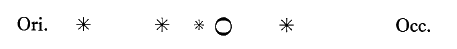
\includegraphics[max width=0.82\textwidth,max height=0.45\textheight,keepaspectratio]{images/figura51.png}\vspace{0.35em}\end{center}
per min. 0, sec. 30, et a recta linea per reliquas Stellas protracta, modicum in aquilonem deflectens: splendidissimæ erant omnes, ac valde conspicuæ. Hora vero quinta cum dimidia, iam Stella orientalis, Iovi proxima, ab illo remotior facta, medium inter ipsum et Stellam orientaliorem, sibi propinquam, obtinebat locum; erantque omnes in eadem recta linea ad unguem, et eiusdem magnitudinis, ut in apposita descriptione videre licet:

\begin{center}\vspace{0.35em}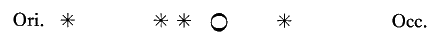
\includegraphics[max width=0.82\textwidth,max height=0.45\textheight,keepaspectratio]{images/figura52.png}\vspace{0.35em}\end{center}
Die duodecima, hora 0, min. 40, Stellæ binæ ab ortu, binæ pariter ab occasu, adstabant. Orientalis remotior a Iove distabat min. 10, longinquior vero occidentalis aberat min. 8,

\begin{center}\vspace{0.35em}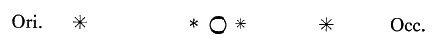
\includegraphics[max width=0.82\textwidth,max height=0.45\textheight,keepaspectratio]{images/figura53.png}\vspace{0.35em}\end{center}
erantque ambæ satis conspicuæ; reliquæ duæ Iovi erant vicinissimæ, et admodum exiguæ, præsertim orientalis, quæ a Iove distabat min. 0, sec. 40; occidentalis vero, min. 1. Hora vero quarta, Stellula, quæ Iovi erat proxima ex oriente, amplius non apparebat.

Die decimatertia, hora 0, min. 30, duæ Stellæ apparebant ab ortu,

\begin{center}\vspace{0.35em}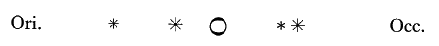
\includegraphics[max width=0.82\textwidth,max height=0.45\textheight,keepaspectratio]{images/figura54.png}\vspace{0.35em}\end{center}
duæ insuper ab occasu. Orientalis ac Iovi vicinior, satis perspicua, distabat ab eo min. 2; ab hac orientalior, minus apparens, aberat min. 4. Ex occidentalibus, remotior a Iove, conspicua valde, ab eo dirimebatur min. 4; inter hanc et Iovem intercidebat Stellula exigua ac occidentaliori Stellæ vicinior, cum ab ea non magis abesset min. 0, sec. 30. Erant omnes in eadem recta secundum Eclipticæ longitudinem ad unguem.

Die decimaquinta (nam decimaquarta Cælum nubibus fuit obductum), hora prima, talis fuit astrorum positus:

\begin{center}\vspace{0.35em}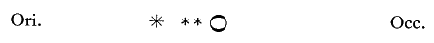
\includegraphics[max width=0.82\textwidth,max height=0.45\textheight,keepaspectratio]{images/figura55.png}\vspace{0.35em}\end{center}
tres nempe erant orientales Stellæ, nulla vero cernebatur occidentalis: orientalis Iovi proxima distabat ab eo min. 0, sec. 50; sequens ab hac aberat min. 0, sec. 20, ab hac vero orientalior min. 2; eratque reliquis maior; viciniores enim Iovi erant admodum exiguæ. Sed, hora proxime quinta, ex Stellis Iovi proximis una tantum cernebatur, a

\begin{center}\vspace{0.35em}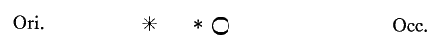
\includegraphics[max width=0.82\textwidth,max height=0.45\textheight,keepaspectratio]{images/figura56.png}\vspace{0.35em}\end{center}
Iove distans min. 0, sec. 30; orientalioris vero elongatio a Iove adaucta erat; fuit enim tunc min. 4. At, hora sexta, præter duas, ut modo dictum est, ab oriente constitutas, una versus occasum cernebatur Stellula, admodum exigua, a Iove remota min. 2.

\begin{center}\vspace{0.35em}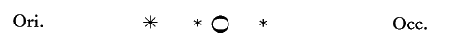
\includegraphics[max width=0.82\textwidth,max height=0.45\textheight,keepaspectratio]{images/figura57.png}\vspace{0.35em}\end{center}
Die decimasexta, hora sexta, in tali constitutione steterunt:

\begin{center}\vspace{0.35em}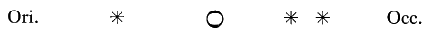
\includegraphics[max width=0.82\textwidth,max height=0.45\textheight,keepaspectratio]{images/figura58.png}\vspace{0.35em}\end{center}
Stella nempe orientalis a Iove min. 7 aberat, Iuppiter a sequenti occidua min. 5, hæc vero a reliqua occidentaliori min. 3: erant omnes eiusdem proxime magnitudinis, satis conspicuæ, et in eadem recta linea exquisite secundum Zodiaci ductum.

Die decimaseptima, hora 1, duæ aderant Stellæ:

\begin{center}\vspace{0.35em}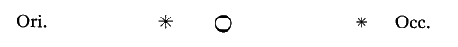
\includegraphics[max width=0.82\textwidth,max height=0.45\textheight,keepaspectratio]{images/figura59.png}\vspace{0.35em}\end{center}
orientalis una, a Iove distans min. 3, occidentalis altera, distans min. 10: hæc erat aliquanto minor orientali. Sed, hora 6, orientalis proximior erat Iovi, distabat nempe min. 0, sec. 50; occidentalis vero remotior fuit, scilicet min. 12. Fuerunt in utraque observatione in eadem recta, et ambæ satis exiguæ, præsertim orientalis in secunda observatione.

Die 18, hora 1, tres aderant Stellæ, quarum duæ occidentales, orientalis vero una: distabat orientalis a Iove min. 3, occidentalis

\begin{center}\vspace{0.35em}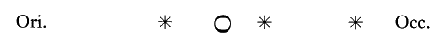
\includegraphics[max width=0.82\textwidth,max height=0.45\textheight,keepaspectratio]{images/figura60.png}\vspace{0.35em}\end{center}
proxima m. 2; occidentalior reliqua aberat a media min. 8: omnes fuerunt in eadem recta ad unguem, et eiusdem fere magnitudinis. At, hora 2, Stellæ viciniores paribus a Iove aberant interstitiis: occidua enim aberat ipsa quoque min. 3. Sed, hora 6, quarta Stellula visa est inter orientaliorem et Iovem, in tali configuratione:

\begin{center}\vspace{0.35em}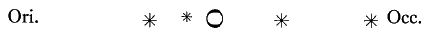
\includegraphics[max width=0.82\textwidth,max height=0.45\textheight,keepaspectratio]{images/figura61.png}\vspace{0.35em}\end{center}
orientalior distabat a sequenti min. 3, sequens a Iove min. 1, sec. 50, Iuppiter ab occidentali sequenti min. 3, hæc vero ab occidentaliori min. 7: erant fere æquales; orientalis tantum Iovi proxima reliquis erat paulo minor: erantque in eadem recta Eclipticæ parallela.

Die 19, hora 0, min. 40, Stellæ duæ solummodo occiduæ a Iove

\begin{center}\vspace{0.35em}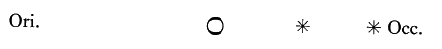
\includegraphics[max width=0.82\textwidth,max height=0.45\textheight,keepaspectratio]{images/figura62.png}\vspace{0.35em}\end{center}
conspectæ fuerunt, satis magnæ, et in eadem recta cum Iove ad unguem, ac secundum Eclipticæ ductum dispositæ. Propinquior a Iove distabat min. 7, hæc vero ab occidentaliori min. 6.

Die 20, nubilosum fuit cælum.

Die 21, hora 1, min. 30, Stellulæ tres satis exiguæ cernebantur in hac constitutione:

\begin{center}\vspace{0.35em}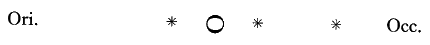
\includegraphics[max width=0.82\textwidth,max height=0.45\textheight,keepaspectratio]{images/figura63.png}\vspace{0.35em}\end{center}
orientalis aberat a Iove min. 2, Iuppiter ab occidentali sequente min. 3, hæc vero ab occidentaliori min. 7: erant ad unguem in eadem recta Eclipticæ parallela.

Die 25, hora 1, min. 30 (nam superioribus tribus noctibus cælum fuit nubibus obductum), tres apparuerunt Stellæ:

\begin{center}\vspace{0.35em}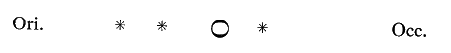
\includegraphics[max width=0.82\textwidth,max height=0.45\textheight,keepaspectratio]{images/figura64.png}\vspace{0.35em}\end{center}
orientales duæ, quarum distantiæ inter se et a Iove æquales fuerunt, ac. min. 4; occidentalis una aberat a Iove min. 2: erant in eadem recta ad unguem, secundum Eclipticæ ductum.

Die 26, hora 0, min. 30, binæ tantum aderant Stellæ:

\begin{center}\vspace{0.35em}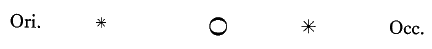
\includegraphics[max width=0.82\textwidth,max height=0.45\textheight,keepaspectratio]{images/figura65.png}\vspace{0.35em}\end{center}
orientalis una, distans a Iove min. 10; occidentalis altera, distans min. 6: orientalis erat aliquanto minor occidentali. Sed hora 5, tres visæ sunt Stellæ:

\begin{center}\vspace{0.35em}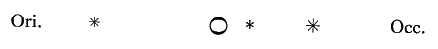
\includegraphics[max width=0.82\textwidth,max height=0.45\textheight,keepaspectratio]{images/figura66.png}\vspace{0.35em}\end{center}
præter enim duas iam adnotatas, tertia ex occidente prope Iovem, admodum exigua, cernebatur, quæ prius sub Iove latitabat, distabatque ab eo min. 1; orientalis vero remotior, quam antea, videbatur, distans nempe a Iove min. 11. Hac nocte primum Iovis et adiacentium planetarum progressum, secundum Zodiaci longitudinem, facta relatione ad fixam quandam, observare placuit: spectabatur enim fixa Stella orientem versus, distans a Planeta orientali min. 11, et paululum in austrum deflectebat, in hunc qui sequitur modum:

\begin{center}\vspace{0.35em}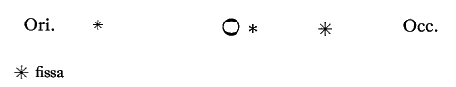
\includegraphics[max width=0.82\textwidth,max height=0.45\textheight,keepaspectratio]{images/figura67.png}\vspace{0.35em}\end{center}
Die 27, hora 1, min. 4, apparebant Stellæ in tali configuratione:

\begin{center}\vspace{0.35em}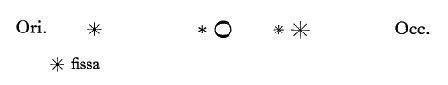
\includegraphics[max width=0.82\textwidth,max height=0.45\textheight,keepaspectratio]{images/figura68.png}\vspace{0.35em}\end{center}
orientalior distabat a Iove min. 10, sequens, Iovi proxima, min. 0, sec. 30; occidentalis sequens aberat min. 2, sec. 30; ab hac occidentalior distabat min. 1. Viciniores Iovi exiguæ apparebant, præsertim orientalis; extremæ vero erant admodum conspicuæ, in primis vero occidua; rectamque lineam secundum Eclipticæ ductum designabant ad unguem. Horum Planetarum progressus versus ortum ex collatione ad praedictam fixam manifeste cernebatur; ipsi enim Iuppiter cum adstantibus Planetis vicinior erat, ut in apposita figura videre licet. Sed hora 5, Stella orientalis Iovi proxima aberat ab eo min. 1.

Die 28, hora 1, duæ tantum Stellæ videbantur; orientalis, distans a Iove min. 9; occidentalis vero, min. 2: erant satis conspicuæ et in eadem recta: ad quam lineam fixa perpendiculariter incidebat in Planetam orientalem, veluti in figura:

\begin{center}\vspace{0.35em}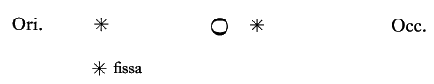
\includegraphics[max width=0.82\textwidth,max height=0.45\textheight,keepaspectratio]{images/figura69.png}\vspace{0.35em}\end{center}
sed, hora 5, tertia Stellula, ex oriente distans a Iove min. 2, conspecta est in eiusmodi constitutione:

\begin{center}\vspace{0.35em}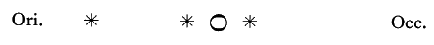
\includegraphics[max width=0.82\textwidth,max height=0.45\textheight,keepaspectratio]{images/figura70.png}\vspace{0.35em}\end{center}
Die 1 Martii, hora 0, min. 40, quatuor Stellæ orientales omnes conspectæ sunt, quarum Iovi proxima aberat ab eo min. 2, sequens ab hac m. 1, tertia m. 0, sec. 2, eratque reliquis clarior; ab ista vero distabat orientalior min. 4, et reliquis erat minor. Rectam proxime designabant lineam, nisi quod tertia a Iove paululum attollebatur. Fixa cum Iove et orientaliori trigonum æquilaterum constituebat, ut in figura:

\begin{center}\vspace{0.35em}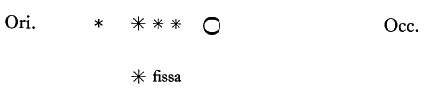
\includegraphics[max width=0.82\textwidth,max height=0.45\textheight,keepaspectratio]{images/figura71.png}\vspace{0.35em}\end{center}
Die 2, hora 0, min. 40, tres adstabant Planetæ, orientales duo, unus vero occiduus, in tali configuratione:

\begin{center}\vspace{0.35em}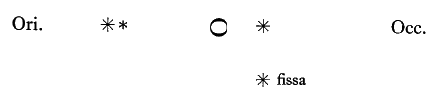
\includegraphics[max width=0.82\textwidth,max height=0.45\textheight,keepaspectratio]{images/figura72.png}\vspace{0.35em}\end{center}
Aberat orientalior a Iove min. 7, ab hoc distabat sequens min. 0, sec. 30; occidentalis vero elongabatur a Iove min. 2: erant extremi lucidiores ac maiores reliquo, qui admodum exiguus apparebat. Orientalior a recta linea, per reliquos et Iovem ducta, paululum in boream videbatur elatus. Fixa iam adnotata ab occidentali Planeta min. 8 distabat, secundum perpendicularem ab ipso Planeta ductam super lineam rectam per Planetas omnes extensam; veluti apposita figura demonstrat.

Hasce Iovis et adiacentium Planetarum ad Fixam collationes apponere placuit, ut ex illis eorundem Planetarum progressus, tum secundum longitudinem, tum etiam secundum latitudinem, cum motibus, qui ex tabulis hauriuntur, ad unguem congruere, quilibet intelligere possit.

Hæ sunt observationes quatuor Mediceorum Planetarum, recens ac primo a me repertorum, ex quibus, quamvis illorum periodos numeris colligere nondum detur, licet saltem quædam animadversione digna pronunciare. Ac primo, cum Iovem consimilibus interstitiis modo consequantur, modo præeant, ab eoque tum versus ortum, tum in occasum angustissimis tantum divaricationibus elongentur, eundemque retrogradum pariter atque directum concomitentur, quin circa illum suas conficiant conversiones, interea dum circa mundi centrum omnes una duodecennales periodos absolvunt, nemini dubium esse potest. Convertuntur insuper in circulis inæqualibus: quod manifeste colligitur ex eo, quia in maioribus a Iove digressionibus nunquam binos Planetas iunctos videre licuit; cum tamen prope Iovem duo, tres et interdum omnes simul constipati reperti sint. Depræhenditur insuper, velociores esse conversiones Planetarum angustiores circa Iovem circulos describentium: propinquiores enim Iovi Stellæ sæpius spectantur orientales, cum pridie ex occasu apparuerint, et e contra: at Planeta, maximum permeans orbem, accurate præadnotatas reversiones perpendenti, restitutiones semimenstruas habere videtur. Eximium præterea præclarumque habemus argumentum pro scrupulo ab illis demendo, qui in Systemate Copernicano conversionem Planetarum circa Solem æquo animo ferentes, adeo perturbantur ab unius Lunæ circa Terram latione, interea dum ambo annuum orbem circa Solem absolvunt, ut hanc universi constitutionem, tanquam impossibilem, evertendam esse arbitrentur: nunc enim, nedum Planetam unum circa alium convertibilem habemus, dum ambo magnum circa Solem perlustrant orbem, verum quatuor circa Iovem, instar Lunæ circa Tellurem, sensus nobis vagantes offert Stellas, dum omnes simul cum Iove, 12 annorum spatio, magnum circa Solem permeant orbem. Prætereundum tandem non est, quanam ratione contingat, ut Medicea Sidera, dum angustissimas circa Iovem rotationes absolvunt, semetipsis interdum plusquam duplo maiora videantur. Causam in vaporibus terrenis minime quærere possumus; apparent enim aucta, seu minuta, dum Iovis et propinquarum fixarum moles nil immutatæ cernuntur. Accedere autem illos, adeoque a terra elongari, circa suæ conversionis perigæum, aut apogæum, ut tantæ mutationis causam nanciscantur, omnino inopinabile videtur: nam arcta circularis latio id nulla ratione præstare valet; ovalis vero motus (qui in hoc casu rectus fere esset) et inopinabilis, et iis quæ apparent nulla ratione consonus, esse videtur. Quod hac in re succurrit, lubens profero, ac recte philosophantium iudicio censuræque exhibeo. Constat, terrestrium vaporum obiectu Solem Lunamque maiores, sed fixas atque Planetas minores, apparere: hinc Luminaria prope horizontem maiora, Stellæ vero, minores ac plerunque inconspicuæ, imminuuntur etiam magis, si iidem vapores lumine fuerint perfusi; idcirco Stellæ interdiu ac intra crepuscula admodum exiles apparent; Luna non item, ut supra quoque monuimus. Constat insuper, non modo Tellurem, sed etiam Lunam, suum habere vaporosum orbem circumfusum, tum ex his quæ supra diximus, tum maxime ex iis, quæ fusius in nostro \textit{Systemate} dicentur: at idem quoque de reliquis Planetis ferre iudicium congrue possumus; adeo ut etiam circa Iovem densiorem reliquo æthere ponere orbem, inopinabile minime videatur; circa quem, instar Lunæ circa elementorum sphæram, Planetæ MEDICEI circumducantur, atque huius orbis obiectu, dum apogæi fuerint, minores, dum vero perigæi, per eiusdem orbis ablationem, seu attenuationem, maiores, appareant. Ulterius progredi temporis angustia inhibet; plura de his brevi candidus Lector expectet.

\end{otherlanguage}
\end{document}
